% Options for packages loaded elsewhere
\PassOptionsToPackage{unicode}{hyperref}
\PassOptionsToPackage{hyphens}{url}
%
\documentclass[
]{article}
\usepackage{lmodern}
\usepackage{amssymb,amsmath}
\usepackage{ifxetex,ifluatex}
\ifnum 0\ifxetex 1\fi\ifluatex 1\fi=0 % if pdftex
  \usepackage[T1]{fontenc}
  \usepackage[utf8]{inputenc}
  \usepackage{textcomp} % provide euro and other symbols
\else % if luatex or xetex
  \usepackage{unicode-math}
  \defaultfontfeatures{Scale=MatchLowercase}
  \defaultfontfeatures[\rmfamily]{Ligatures=TeX,Scale=1}
\fi
% Use upquote if available, for straight quotes in verbatim environments
\IfFileExists{upquote.sty}{\usepackage{upquote}}{}
\IfFileExists{microtype.sty}{% use microtype if available
  \usepackage[]{microtype}
  \UseMicrotypeSet[protrusion]{basicmath} % disable protrusion for tt fonts
}{}
\makeatletter
\@ifundefined{KOMAClassName}{% if non-KOMA class
  \IfFileExists{parskip.sty}{%
    \usepackage{parskip}
  }{% else
    \setlength{\parindent}{0pt}
    \setlength{\parskip}{6pt plus 2pt minus 1pt}}
}{% if KOMA class
  \KOMAoptions{parskip=half}}
\makeatother
\usepackage{xcolor}
\IfFileExists{xurl.sty}{\usepackage{xurl}}{} % add URL line breaks if available
\IfFileExists{bookmark.sty}{\usepackage{bookmark}}{\usepackage{hyperref}}
\hypersetup{
  pdftitle={Documentación de usuario},
  hidelinks,
  pdfcreator={LaTeX via pandoc}}
\urlstyle{same} % disable monospaced font for URLs
\usepackage{color}
\usepackage{fancyvrb}
\newcommand{\VerbBar}{|}
\newcommand{\VERB}{\Verb[commandchars=\\\{\}]}
\DefineVerbatimEnvironment{Highlighting}{Verbatim}{commandchars=\\\{\}}
% Add ',fontsize=\small' for more characters per line
\newenvironment{Shaded}{}{}
\newcommand{\AlertTok}[1]{\textcolor[rgb]{1.00,0.00,0.00}{\textbf{#1}}}
\newcommand{\AnnotationTok}[1]{\textcolor[rgb]{0.38,0.63,0.69}{\textbf{\textit{#1}}}}
\newcommand{\AttributeTok}[1]{\textcolor[rgb]{0.49,0.56,0.16}{#1}}
\newcommand{\BaseNTok}[1]{\textcolor[rgb]{0.25,0.63,0.44}{#1}}
\newcommand{\BuiltInTok}[1]{#1}
\newcommand{\CharTok}[1]{\textcolor[rgb]{0.25,0.44,0.63}{#1}}
\newcommand{\CommentTok}[1]{\textcolor[rgb]{0.38,0.63,0.69}{\textit{#1}}}
\newcommand{\CommentVarTok}[1]{\textcolor[rgb]{0.38,0.63,0.69}{\textbf{\textit{#1}}}}
\newcommand{\ConstantTok}[1]{\textcolor[rgb]{0.53,0.00,0.00}{#1}}
\newcommand{\ControlFlowTok}[1]{\textcolor[rgb]{0.00,0.44,0.13}{\textbf{#1}}}
\newcommand{\DataTypeTok}[1]{\textcolor[rgb]{0.56,0.13,0.00}{#1}}
\newcommand{\DecValTok}[1]{\textcolor[rgb]{0.25,0.63,0.44}{#1}}
\newcommand{\DocumentationTok}[1]{\textcolor[rgb]{0.73,0.13,0.13}{\textit{#1}}}
\newcommand{\ErrorTok}[1]{\textcolor[rgb]{1.00,0.00,0.00}{\textbf{#1}}}
\newcommand{\ExtensionTok}[1]{#1}
\newcommand{\FloatTok}[1]{\textcolor[rgb]{0.25,0.63,0.44}{#1}}
\newcommand{\FunctionTok}[1]{\textcolor[rgb]{0.02,0.16,0.49}{#1}}
\newcommand{\ImportTok}[1]{#1}
\newcommand{\InformationTok}[1]{\textcolor[rgb]{0.38,0.63,0.69}{\textbf{\textit{#1}}}}
\newcommand{\KeywordTok}[1]{\textcolor[rgb]{0.00,0.44,0.13}{\textbf{#1}}}
\newcommand{\NormalTok}[1]{#1}
\newcommand{\OperatorTok}[1]{\textcolor[rgb]{0.40,0.40,0.40}{#1}}
\newcommand{\OtherTok}[1]{\textcolor[rgb]{0.00,0.44,0.13}{#1}}
\newcommand{\PreprocessorTok}[1]{\textcolor[rgb]{0.74,0.48,0.00}{#1}}
\newcommand{\RegionMarkerTok}[1]{#1}
\newcommand{\SpecialCharTok}[1]{\textcolor[rgb]{0.25,0.44,0.63}{#1}}
\newcommand{\SpecialStringTok}[1]{\textcolor[rgb]{0.73,0.40,0.53}{#1}}
\newcommand{\StringTok}[1]{\textcolor[rgb]{0.25,0.44,0.63}{#1}}
\newcommand{\VariableTok}[1]{\textcolor[rgb]{0.10,0.09,0.49}{#1}}
\newcommand{\VerbatimStringTok}[1]{\textcolor[rgb]{0.25,0.44,0.63}{#1}}
\newcommand{\WarningTok}[1]{\textcolor[rgb]{0.38,0.63,0.69}{\textbf{\textit{#1}}}}
\usepackage{longtable,booktabs}
% Correct order of tables after \paragraph or \subparagraph
\usepackage{etoolbox}
\makeatletter
\patchcmd\longtable{\par}{\if@noskipsec\mbox{}\fi\par}{}{}
\makeatother
% Allow footnotes in longtable head/foot
\IfFileExists{footnotehyper.sty}{\usepackage{footnotehyper}}{\usepackage{footnote}}
\makesavenoteenv{longtable}
\usepackage{graphicx}
\makeatletter
\def\maxwidth{\ifdim\Gin@nat@width>\linewidth\linewidth\else\Gin@nat@width\fi}
\def\maxheight{\ifdim\Gin@nat@height>\textheight\textheight\else\Gin@nat@height\fi}
\makeatother
% Scale images if necessary, so that they will not overflow the page
% margins by default, and it is still possible to overwrite the defaults
% using explicit options in \includegraphics[width, height, ...]{}
\setkeys{Gin}{width=\maxwidth,height=\maxheight,keepaspectratio}
% Set default figure placement to htbp
\makeatletter
\def\fps@figure{htbp}
\makeatother
\setlength{\emergencystretch}{3em} % prevent overfull lines
\providecommand{\tightlist}{%
  \setlength{\itemsep}{0pt}\setlength{\parskip}{0pt}}
\setcounter{secnumdepth}{-\maxdimen} % remove section numbering

\title{Documentación de usuario}
\author{}
\date{}

\begin{document}
\maketitle

\hypertarget{introducciuxf3n}{%
\section{Introducción}\label{introducciuxf3n}}

En este apartado se pretende dotar al usuario de la información
necesaria para la correcta utilización de la aplicación. En primer
lugar, se especificarán los requisitos \emph{software} con los que el
usuario debe contar para acceder a la aplicación. Posteriormente, se
explicará paso a paso el proceso de instalación y, finalmente, se
mostrará el manual de usuario.

\hypertarget{requisitos-de-usuario}{%
\section{Requisitos de usuario}\label{requisitos-de-usuario}}

Los requisitos de usuario varían en función del modo de instalación que
vaya a llevar a cabo el usuario. Existen tres modos de instalación:
Manual, \emph{Docker} y \emph{Kubernetes}.

Como es lógico, además de los requisitos que se van a mostrar a
continuación, se debe contar con un \textbf{navegador web} desde el que
se pueda acceder a la aplicación web.

\hypertarget{manual}{%
\subsection{Manual}\label{manual}}

Si se escoge la opción manual hay que estar seguro de que el servidor
cumple con todos y cada uno de los siguientes \textbf{requisitos}:

\begin{itemize}
\item
  Sistema Operativo Linux
\item
  Apache HTTP Server (con el módulo \emph{rewrite} activado)
\item
  MySQL / MariaDB v5.0 o superior.
\item
  PHP v5.4 o superior con las sisguientes extensiones instaladas:

  \begin{quote}
  \begin{itemize}
  \tightlist
  \item
    mysqli
  \item
    exif
  \item
    curl
  \item
    mbstring
  \end{itemize}
  \end{quote}
\item
  ImageMagick (Tratamiento de imágenes)
\end{itemize}

* \href{http://httpd.apache.org/docs/trunk/es/install.html}{HTTP Apache
Server} *
\href{https://dev.mysql.com/doc/mysql-installation-excerpt/5.7/en/}{MySQL}
* \href{https://www.php.net/manual/es/install.php}{PHP} *
\href{https://imagemagick.org/script/install-source.php}{ImageMagick}

\hypertarget{docker}{%
\subsection{Docker}\label{docker}}

En este caso, solo es necesario un único \textbf{requisito}:

\begin{itemize}
\tightlist
\item
  \emph{Docker} (Probado con la versión 19.03.6).
\end{itemize}

* \href{https://docs.docker.com/engine/install/}{Docker Engine}

\hypertarget{kubernetes}{%
\subsection{Kubernetes}\label{kubernetes}}

Si se pretende utilizar \emph{Kubernetes} para el despliegue de la
infraestructura se requiere:

\begin{itemize}
\tightlist
\item
  \emph{Docker}
\item
  La herramienta de línea de comandos de \emph{Kubernetes},
  \emph{kubectl} (Probado en v1.18.2).
\item
  \emph{Kustomize} (probado en v3.1.0)
\end{itemize}

* \href{https://docs.docker.com/engine/install/}{Docker Engine} *
\href{https://kubernetes.io/es/docs/tasks/tools/install-kubectl/}{Kubernetes}
* \href{https://github.com/kubernetes-sigs/kustomize}{Kustomize}

\hypertarget{instalaciuxf3n}{%
\section{Instalación}\label{instalaciuxf3n}}

Como se ha comentado en el apartado anterior, existen tres posibilidades
distintas para instalar la aplicación en un servidor: \emph{Manual},
\emph{Docker} o \emph{Kubernetes}.

\hypertarget{manual-1}{%
\subsection{Manual}\label{manual-1}}

Note

Para el siguiente tutorial se ha utilizado como S.O Ubuntu 19.10

Warning

¡ Es muy importante comprobar que se cumplen todos los
\protect\hyperlink{requisitos-de-usuario}{Requisitos de usuario} !

El primer paso consiste en \textbf{configurar el servidor}. Para ello,
hay que seguir una serie de indicaciones:

\begin{enumerate}
\def\labelenumi{\arabic{enumi}.}
\tightlist
\item
  \textbf{Crear la base de datos (DB) MySQL} desde un usuario con
  permisos suficientes como para poder realizar operaciones sobre ella.

  \begin{itemize}
  \item
    Durante el proceso, conviene apuntar los siguientes datos:

    \begin{quote}
    \begin{itemize}
    \tightlist
    \item
      \emph{Hostname} donde se encuentra alojada la DB.
    \item
      Nombre de la DB.
    \item
      Nombre del usuario de la DB.
    \item
      Contraseña de usuario de la DB.
    \end{itemize}
    \end{quote}
  \item
    La base de datos ha de estar codificada en {utf8}.
  \end{itemize}
\end{enumerate}

\begin{verbatim}
sudo mysql -u root -
CREATE DATABASE omekadb CHARACTER SET utf8mb4 COLLATE utf8mb4_unicode_ci;
CREATE USER 'usuario'@'localhost' IDENTIFIED BY 'contraseña';
GRANT ALL ON omeka.* TO 'usuario'@'localhost' IDENTIFIED BY 'contraseña' WITH GRANT OPTION;
FLUSH PRIVILEGES;
EXIT;
\end{verbatim}

\begin{enumerate}
\def\labelenumi{\arabic{enumi}.}
\setcounter{enumi}{1}
\tightlist
\item
  \textbf{Descargar} la version 2.7.1 de \textbf{Omeka}, desde su {[}web
  oficial{]}(\url{https://omeka.org/classic/download/}) o desde su
  {[}repositorio oficial{]}(\url{http://github.com/omeka/Omeka}) en
  GitHub.
\end{enumerate}

\begin{verbatim}
cd /tmp && wget https://github.com/omeka/Omeka/releases/download/v2.7.1/omeka-2.7.1.zip
\end{verbatim}

\begin{enumerate}
\def\labelenumi{\arabic{enumi}.}
\setcounter{enumi}{2}
\tightlist
\item
  \textbf{Descomprimir} el fichero {.zip} recién descargado sobre un
  directorio desde donde podamos trabajar.
\end{enumerate}

\begin{verbatim}
unzip omeka-2.7.1.zip -d <directorio_de_trabajo>
\end{verbatim}

\begin{enumerate}
\def\labelenumi{\arabic{enumi}.}
\setcounter{enumi}{3}
\tightlist
\item
  Desde el directorio escogido, buscar el fichero {db.ini} y
  \textbf{sustituir los valores 'XXXXX' por los datos de la base de
  datos} (anotados en el paso 1).
\end{enumerate}

\begin{verbatim}
cd <directorio_de_trabajo>
nano db.ini

No es necesario modificar los parámetros `prefix` o `port`.
\end{verbatim}

\begin{verbatim}
;;;;;;;;;;;;;;;;;;;;;;;;;;;;;;;
; Database Configuration File ;
;;;;;;;;;;;;;;;;;;;;;;;;;;;;;;;
;
; Omeka requires MySQL 5 or newer.
;
; To configure your database, replace the X's with your specific
; settings. If you're unsure about your database information, ask
; your server administrator, or consult the documentation at
; <http://omeka.org/codex/Database_Configuration_File>.

[database]
host     = "localhost"
username = "usuario"
password = "contraseña"
dbname   = "omekadb"
prefix   = "omeka_"
charset  = "utf8"
;port     = ""
\end{verbatim}

\begin{enumerate}
\def\labelenumi{\arabic{enumi}.}
\setcounter{enumi}{4}
\tightlist
\item
  \textbf{Descargar} el contenido del
  \href{https://github.com/gcm1001/TFG-CeniehAriadne}{repositorio del
  proyecto}.
\end{enumerate}

\begin{verbatim}
cd /tmp && wget https://github.com/gcm1001/TFG-CeniehAriadne/archive/master.zip
\end{verbatim}

\begin{enumerate}
\def\labelenumi{\arabic{enumi}.}
\setcounter{enumi}{5}
\tightlist
\item
  \textbf{Descomprimir} las carpetas {/omeka/plugins} y {/omeka/themes}
  del fichero {.zip} recién descargado.
\end{enumerate}

\begin{verbatim}
unzip master.zip 'TFG-CeniehAriadne-master/omeka/plugins/*' 'TFG-CeniehAriadne-master/omeka/themes/*' -d <*directorio_de_trabajo*>
\end{verbatim}

\begin{enumerate}
\def\labelenumi{\arabic{enumi}.}
\setcounter{enumi}{6}
\tightlist
\item
  Desde el directorio de trabajo, \textbf{reemplazar las carpetas
  originales} \emph{plugins} y \emph{themes} por las previamente
  descargadas.
\end{enumerate}

\begin{verbatim}
cd <*directorio_de_trabajo*>
rm -rf ./plugins ./themes
sudo cp -r ./TFG-CeniehAriadne-master/omeka/* .
rm -rf ./TFG-CeniehAriadne-master
\end{verbatim}

\begin{enumerate}
\def\labelenumi{\arabic{enumi}.}
\setcounter{enumi}{7}
\tightlist
\item
  Mover todo el contenido del directorio de trabajo a la carpeta del
  servidor Apache.
\end{enumerate}

\begin{verbatim}
mv -r <*directorio_de_trabajo*>/* <*directorio_del_servidor*>
\end{verbatim}

\begin{enumerate}
\def\labelenumi{\arabic{enumi}.}
\setcounter{enumi}{8}
\tightlist
\item
  \textbf{Dar permisos de lectura y escritura sobre todo el contenido de
  la aplicación}.
\end{enumerate}

\begin{verbatim}
cd <*directorio_del_servidor*>
sudo chown -R www-data:www-data <*directorio_de_trabajo*>
sudo chmod -R 755 <*directorio_de_trabajo*>
\end{verbatim}

\begin{enumerate}
\def\labelenumi{\arabic{enumi}.}
\setcounter{enumi}{9}
\tightlist
\item
  \textbf{Configurar el servidor Apache}:
\end{enumerate}

\begin{quote}
10.1. \textbf{Crear el archivo de configuración} correspondiente a la
aplicación.

\begin{verbatim}
nano /etc/apache2/sites-available/omeka.conf
\end{verbatim}

Cambiar los valores "\emph{DocumentRoot}" y "\emph{ServerName}". ..
code-block:

\begin{verbatim}
<VirtualHost *:80>
     ServerAdmin [email protected]
     DocumentRoot <directorio_del_servidor>
     ServerName <nombre_del_servidor>

     <Directory /var/www/html/omeka/>
          Options FollowSymlinks
          AllowOverride All
          Require all granted
     </Directory>

     ErrorLog ${APACHE_LOG_DIR}/error.log
     CustomLog ${APACHE_LOG_DIR}/access.log combined

</VirtualHost>
\end{verbatim}

\begin{enumerate}
\def\labelenumi{\alph{enumi}.}
\setcounter{enumi}{1}
\tightlist
\item
  \textbf{*Activar el sitio y el módulo rewrite} y \textbf{reiniciar el
  servidor} para aplicar los cambios.
\end{enumerate}

\begin{verbatim}
a2ensite omeka.conf
a2enmod rewrite
systemctl restart apache2.service
\end{verbatim}
\end{quote}

Desde este instante, \textbf{la aplicación será accesible desde el
navegador} (puerto 80). El último paso consiste en \textbf{completar la
instalación guiada desde el navegador}, disponible en el directorio
{/install} (e.g \emph{http://aplicacion.es/install}).

Una vez instalada la aplicación, para poder disfrutar de todas las
mejoras propuestas en este proyecto, se deben instalar tanto los
\emph{plugins} como el tema propuesto (ver
\protect\hyperlink{instalar-complementos-plugins}{Instalar complementos
(plugins)} e \protect\hyperlink{instalar-temas-themes}{Instalar temas
(themes)})

Warning

Por temas de seguridad, conviene eliminar la carpeta {/install/} del
directorio raíz una vez terminada la instalación de la aplicación.

* \href{https://omeka.org/classic/docs/Installation/Installation/}{Omeka
Classic User Manual}

\hypertarget{docker-1}{%
\subsection{Docker}\label{docker-1}}

Warning

¡ Es muy importante comprobar que se cumplen todos los
\protect\hyperlink{requisitos-de-usuario}{Requisitos de usuario} !

Note

Para el siguiente tutorial se ha utilizado como S.O Ubuntu 19.10

Para proceder al despliegue \textbf{se deben descargar}, del
\href{https://github.com/gcm1001/TFG-CeniehAriadne}{repositorio del
proyecto}, los siguientes ficheros:

\begin{itemize}
\tightlist
\item
  {/Dockerfile}
\item
  {/docker-compose.yml}
\item
  {/ConfigFiles/*}
\item
  {/omeka/plugins/*}
\end{itemize}

Warning

Mantén los subdirectorios intactos.

A continuación debes \textbf{compilar la imagen}. Para ello, desde el
directorio donde hayas almacenado la descarga anterior, ejecuta el
siguiente comando:

\begin{Shaded}
\begin{Highlighting}[]
\ExtensionTok{docker}\NormalTok{ build {-}t nombre\_imagen:tag .}
\end{Highlighting}
\end{Shaded}

\textbf{Recuerda muy bien el nombre de la imagen y el tag que pongas}
porque será necesario para el siguiente paso, que consiste en configurar
el archivo {docker-compose.yml}.

En él, solo tenemos que cambiar la etiqueta {image} del servicio
{omeka\_app} con el nombre y el tag de la imagen recién compilada:

\begin{Shaded}
\begin{Highlighting}[]
\ExtensionTok{...}
  \ExtensionTok{omeka\_app}\NormalTok{:}
    \ExtensionTok{image}\NormalTok{: nombre\_imagen:tag}
\end{Highlighting}
\end{Shaded}

Si se ha publicado la imagen en \emph{DockerHub}, se puede hacer
referencia a esta indicando el nombre de usuario seguido de la imagen
(e.g. username/nombre\_de\_mi\_imagen:tag).

Warning

Elimina el servicio {omeka-db-admin} si tu servidor está destinado a
producción. Este servicio incorpora la herramienta \emph{PhpMyAdmin} a
la infraestructura, la cual tiene un alto grado de vulnerabilidades.

Por último, crear los \emph{secrets} correspondientes a las contraseñas
de la base de datos:

\begin{Shaded}
\begin{Highlighting}[]
\BuiltInTok{echo} \StringTok{\textquotesingle{}contraseña\_usuario\_db\textquotesingle{}} \KeywordTok{|} \ExtensionTok{docker}\NormalTok{ secret create omeka\_db\_password {-}}
\BuiltInTok{echo} \StringTok{\textquotesingle{}contraseña\_root\_db\textquotesingle{}} \KeywordTok{|} \ExtensionTok{docker}\NormalTok{ secret create omeka\_db\_root\_password {-}}
\FunctionTok{cp}\NormalTok{ configFiles/db.ini.example configFiles/db.ini}
\end{Highlighting}
\end{Shaded}

Warning

Debes modificar el fichero recién creado {db.ini} con los datos de la
base de datos. Ten en cuenta que la contraseña que introduzcas en el
fichero tiene que coincidir con la del \emph{secret} recién creado.

Ahora ya se puede desplegar la infraestructura ejecutando el siguiente
comando desde el directorio de trabajo (donde se encuentra la descarga
del primer paso).

\begin{Shaded}
\begin{Highlighting}[]
\ExtensionTok{docker}\NormalTok{ stack deploy {-}c docker{-}compose.yml nombre\_del\_entorno}
\end{Highlighting}
\end{Shaded}

Desde este instante la aplicación es accesible desde el navegador
(puerto 80). Los siguientes pasos son los mismos que en la
\href{Manual}{instalación manual}.

\hypertarget{kubernetes-1}{%
\subsection{Kubernetes}\label{kubernetes-1}}

Warning

¡ Es muy importante comprobar que se cumplen todos los
\protect\hyperlink{requisitos-de-usuario}{Requisitos de usuario} !

Note

Para el siguiente tutorial se ha utilizado como S.O Ubuntu 19.10

El primer paso para desplegar la aplicación mediante \emph{Kubernetes}
es montar nuestra imagen \emph{Docker} (Sigue los primeros pasos del
punto anterior, \textbf{hasta la compilación de la imagen}).

El siguiente paso consiste en desplegar la aplicación. Para esta tarea
utilizo el gestor de objetos \emph{Kustomize}. Por ello, deberás contar
con dicha herramienta. Además debes estar en posesión de los siguientes
ficheros alojados en este repositorio:

\begin{itemize}
\tightlist
\item
  /kustomization.yaml
\item
  /patch.yaml
\item
  /gke-mysql/*
\item
  /gke-omeka/*
\item
  /configFiles/db.ini
\end{itemize}

Ahora, debes crear el {secret} que contendrá todos los datos privados
necesarios para crear la la base de datos (nombre de la base de datos,
nombre de usuario, contraseña de usuario y contraseña root).

Warning

Antes de ejecutar los siguientes comandos debes crear las
\emph{variables de entorno} que se están utilizando: DB\_PASSWORD,
DB\_ROOT\_PASSWORD, DB\_USERNAME y DB\_DATABASE.

\begin{verbatim}
kubectl create secret omeka-db \
--from-literal=user-password=$DB_PASSWORD \
--from-literal=root-password=$DB_ROOT_PASSWORD \
--from-literal=username=$DB_USERNAME \
--from-literal=database=$DB_DATABASE
\end{verbatim}

Además debemos crear el \emph{configmap} que almacenará todo el
contenido del fichero de configuración {db.ini} (no necesitas
modificarlo ya que este emplea las variables de entorno utilizadas en
los comandos anteriores).

\begin{verbatim}
kubectl create configmap db-config \
--from-file ./configFiles/db.ini
\end{verbatim}

Por último, debemos indicar el identificador de nuestra imagen
\emph{Docker} en el fichero {/gke-omeka/deployment.yaml}.

\begin{Shaded}
\begin{Highlighting}[]
\ExtensionTok{...}
    \ExtensionTok{spec}\NormalTok{:}
      \ExtensionTok{containers}\NormalTok{:}
      \ExtensionTok{{-}}\NormalTok{ image: nombre\_imagen:tag}
\ExtensionTok{...}
\end{Highlighting}
\end{Shaded}

Tras esto, solo faltaría ejecutar, desde el directorio raíz, el
siguiente comando:

\begin{Shaded}
\begin{Highlighting}[]
\ExtensionTok{kustomize}\NormalTok{ build . }\KeywordTok{|} \ExtensionTok{kubectl}\NormalTok{ apply {-}f {-}}
\end{Highlighting}
\end{Shaded}

Desde este instante la aplicación es accesible desde el navegador
(puerto 80). Los siguientes pasos son los mismos que en la
\href{Manual}{instalación manual}.

\hypertarget{manual-de-usuario}{%
\section{Manual de usuario}\label{manual-de-usuario}}

Warning

Este manual de usuario \textbf{no es válido para la versión original} de
\href{https://omeka.org/classic}{Omeka Classic}. Ciertos aspectos de la
aplicación han sido alterados por los complementos/\emph{plugins}
instalados y el tema escogido. Por lo tanto, antes de seguir leyendo,
comprueba que se ha instalado el tema y todos los \emph{plugins}
indicados en el apartado
\protect\hyperlink{instalaciuxf3n}{Instalación}.

Note

Para acceder al \textbf{manual de usuario original}, pulsa
\href{https://omeka.org/classic/docs/}{aquí}.

\hypertarget{uxe1rea-de-administraciuxf3n}{%
\subsection{Área de administración}\label{uxe1rea-de-administraciuxf3n}}

La zona de administración es el lugar desde donde el cual se gestionan
los conjuntos de datos almacenados en la plataforma y, además, se pueden
configurar otros aspectos de la aplicación como, por ejemplo, su diseño,
seguridad, usuarios, etc.

Este área se encuentra ubicado en la ruta {/admin} desde la raíz del
directorio donde se encuentra la aplicación. Si, por ejemplo, hemos
accedido desde la URL {www.aplicacion.es}, al acceder a
{www.aplicacion.es/admin} se nos mostrará la pantalla de inicio de
sesión al sistema.

\begin{figure}
\hypertarget{admin-login}{%
\centering
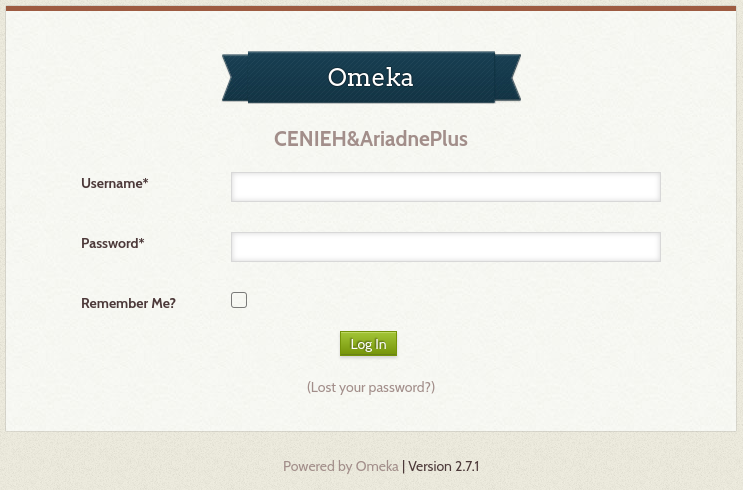
\includegraphics{../_static/images/admin-login.png}
\caption{Inicio de sesión del área de administración}\label{admin-login}
}
\end{figure}

Después de introducir un nombre de usuario y contraseña válidos, se debe
pulsar sobre el botón "\emph{Login}". Si todo es correcto, accederemos
al interior de la zona de administración.

\hypertarget{menuxfas-de-navegaciuxf3n}{%
\subsubsection{Menús de navegación}\label{menuxfas-de-navegaciuxf3n}}

Dentro del área de administración podemos desplazarnos a través de los
dos menús de navegación disponibles:

\begin{figure}
\hypertarget{admin-view}{%
\centering
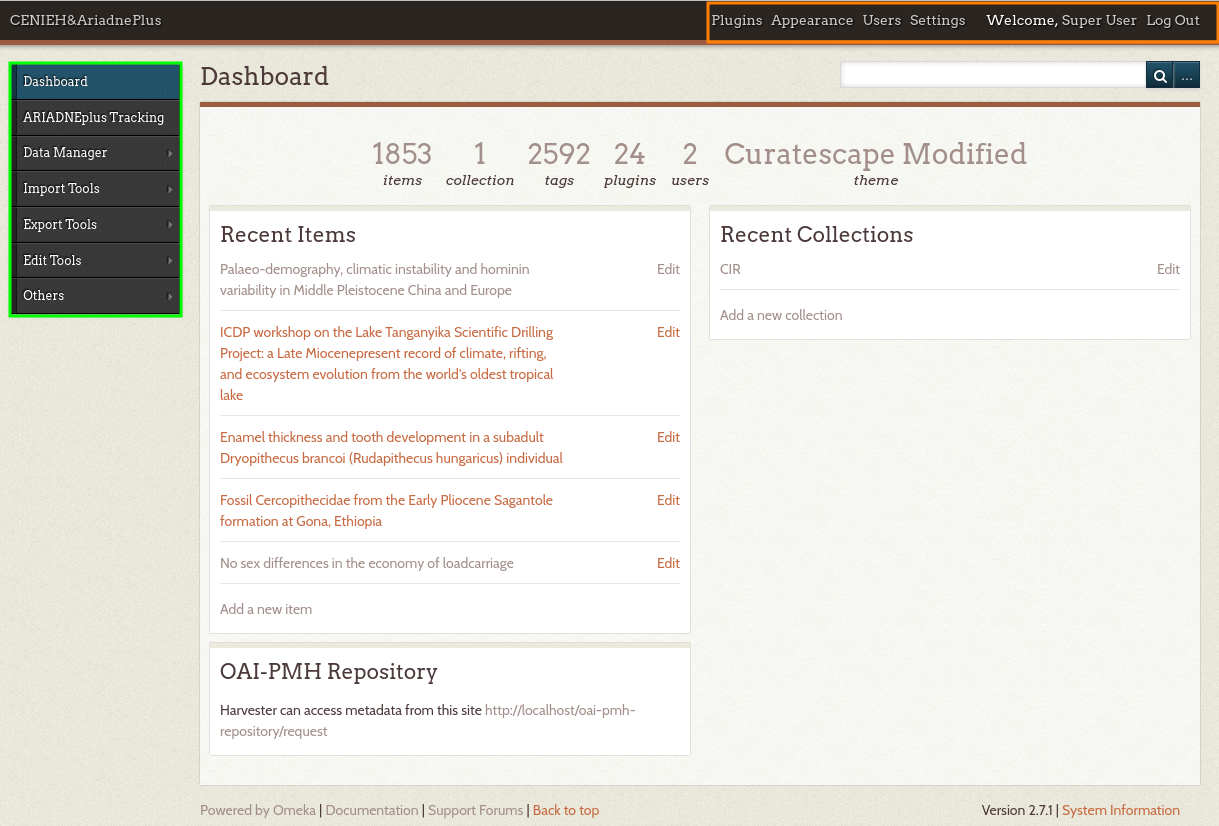
\includegraphics{../_static/images/admin-view.png}
\caption{Vista principal del panel de administración}\label{admin-view}
}
\end{figure}

\begin{enumerate}
\def\labelenumi{\arabic{enumi}.}
\tightlist
\item
  \textbf{Menú global}: recoge los accesos hacia las principales zonas
  de configuración de la aplicación.

  \begin{enumerate}
  \def\labelenumii{\alph{enumii}.}
  \tightlist
  \item
    \emph{Plugins}: zona donde se gestionan complementos/\emph{plugins}.
  \item
    \emph{Appearance}: zona donde se gestionan temas de diseño.
  \item
    \emph{Users}: zona donde se gestionan usuarios.
  \item
    \emph{Settings} zona donde se gestiona la configuración de la
    aplicación.
  \end{enumerate}
\item
  \textbf{Menú principal}: a través de este menú se puede acceder a cada
  una de las funciones/complementos incluídos en la plataforma.

  \begin{enumerate}
  \def\labelenumii{\alph{enumii}.}
  \tightlist
  \item
    \emph{Dashboard}: recoge información general de la aplicación
    (número de ítems/coleciones almacenadas, \emph{tags}, etc.).
  \item
    \emph{ARIADNEplus Tracking}: zona donde se gestionan los procesos de
    integración de datos a la plataforma ARIADNEplus.
  \item
    \emph{Data Manager}: zona donde se gestionan los objetos principales
    de la aplicación (ítems, tipo de ítems, ficheros, colecciones y
    tags).
  \item
    \emph{Import Tools}: recoge las distintas herramientas de
    importación.
  \item
    \emph{Export Tools}: recoge las distintas herramientas de
    exportación.
  \item
    \emph{Edit Tools}: recoge las distintas herramientas de edición de
    objetos.
  \item
    \emph{Others}: recoge herramientas auxiliares.
  \end{enumerate}
\end{enumerate}

\hypertarget{gestionar-complementos-plugins}{%
\subsubsection{\texorpdfstring{Gestionar complementos
(\emph{plugins})}{Gestionar complementos (plugins)}}\label{gestionar-complementos-plugins}}

La principal ventaja de esta aplicación es que puedes añadir nuevas
funciones a través de los complementos o \emph{plugins}. A través de la
entrada \emph{Plugins} del menú global, se accede al gestor de
\emph{plugins} ({/admin/plugins}), lugar donde se llevan a cabo todas
las tareas de gestión relacionadas con este tipo de aplicaciones.

\hypertarget{instalar-complementos-plugins}{%
\paragraph{\texorpdfstring{Instalar complementos
(\emph{plugins})}{Instalar complementos (plugins)}}\label{instalar-complementos-plugins}}

Warning

Si se siguieron a rajatabla los pasos de la
\protect\hyperlink{instalaciuxf3n}{Instalación}, la aplicación ya cuenta
con los \emph{plugins} propuestos dentro de la carpeta {/plugins/}. Por
lo tanto, puedes saltarte el primer paso que ves a continuación e ir
directamente a los puntos de instalación. \textbf{Para obtener más
información de los complementos propuestos, ver el apartado}
\protect\hyperlink{complementos-plugins}{Complementos (plugins)} .

El primer paso para instalar cualquier complemento, es descargarlo.
Actualmente existen dos sitios desde donde se pueden obtener
\emph{plugins}:

\begin{enumerate}
\def\labelenumi{\arabic{enumi}.}
\tightlist
\item
  \href{https://omeka.org/classic/plugins/}{Página oficial de Omeka}
\item
  \href{https://daniel-km.github.io/UpgradeToOmekaS/omeka_plugins.html}{Repositorio
  de Github}
\end{enumerate}

Una vez descargado, se debe transportar la carpeta del \emph{plugin}
correspondiente a la carpeta {/plugins/} del directorio raíz de la
aplicación.

Con los \emph{plugins} ya almacenados en la aplicación, se puede llevar
a cabo el proceso de instalación desde la plataforma.

Para instalar un complemento (\emph{plugin}):

\begin{enumerate}
\def\labelenumi{\arabic{enumi}.}
\tightlist
\item
  Desde el gestor de \emph{plugins} ({/admin/plugins}).
\item
  Localizar el nombre del complemento que se desea instalar.
\item
  Hacer clic sobre el botón "\emph{Install}".
\end{enumerate}

\begin{figure}
\hypertarget{plugins-inst}{%
\centering
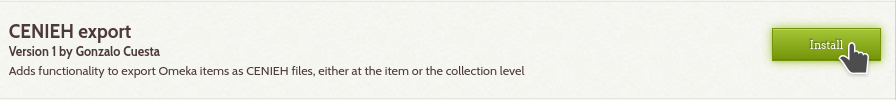
\includegraphics{../_static/images/plugins-inst.png}
\caption{}\label{plugins-inst}
}
\end{figure}

\begin{enumerate}
\def\labelenumi{\arabic{enumi}.}
\setcounter{enumi}{3}
\tightlist
\item
  En caso de que el \emph{plugin} sea configurable, rellenar el
  formulario de configuración y hacer clic en el botón "\emph{Save
  Changes}".
\end{enumerate}

\hypertarget{configurar-complementos-plugins}{%
\paragraph{\texorpdfstring{Configurar complementos
(\emph{plugins})}{Configurar complementos (plugins)}}\label{configurar-complementos-plugins}}

Algunos complementos ofrecen la posibilidad de configurar la
funcionalidad que implementan.

Para configurar un complemento (\emph{plugin}):

\begin{enumerate}
\def\labelenumi{\arabic{enumi}.}
\tightlist
\item
  Desde el gestor de \emph{plugins} ({/admin/plugins}).
\item
  Localizar el nombre del complemento que se desea configurar.
\item
  Hacer clic sobre el botón "\emph{Configure}".
\end{enumerate}

\begin{figure}
\hypertarget{plugins-conf-1}{%
\centering
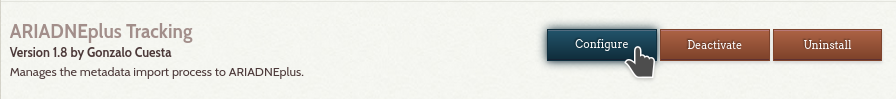
\includegraphics{../_static/images/plugins-conf-1.png}
\caption{}\label{plugins-conf-1}
}
\end{figure}

\begin{enumerate}
\def\labelenumi{\arabic{enumi}.}
\setcounter{enumi}{3}
\tightlist
\item
  Modificar el formulario de configuración y hacer clic en el botón
  "\emph{Save Changes}".
\end{enumerate}

\begin{figure}
\hypertarget{plugins-conf-2}{%
\centering
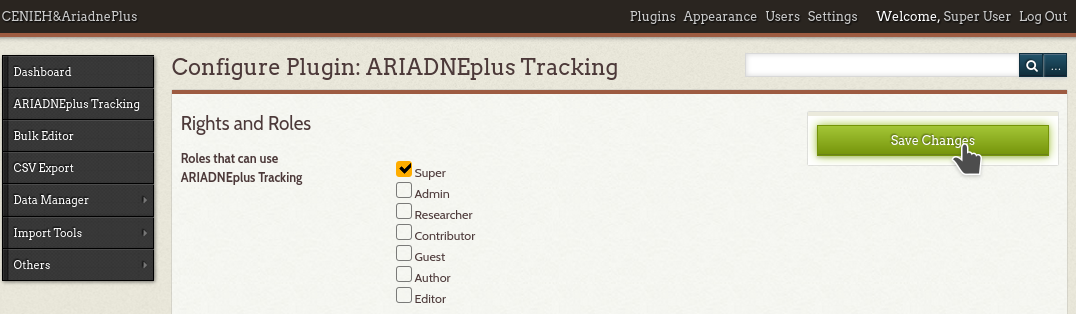
\includegraphics{../_static/images/plugins-conf-2.png}
\caption{}\label{plugins-conf-2}
}
\end{figure}

\hypertarget{activardesactivar-complementos-plugins}{%
\paragraph{\texorpdfstring{Activar/Desactivar complementos
(\emph{plugins})}{Activar/Desactivar complementos (plugins)}}\label{activardesactivar-complementos-plugins}}

Al desactivar un complemento, todas las funciones que incluía en la
aplicación desaparecen.

Para activar/desactivar un complemento (\emph{plugin}):

\begin{enumerate}
\def\labelenumi{\arabic{enumi}.}
\tightlist
\item
  Desde el gestor de \emph{plugins} ({/admin/plugins}).
\item
  Localizar el nombre del complemento que se desea configurar.
\item
  Hacer clic sobre el botón "\emph{Deactivate}" para desactivar o sobre
  el botón "\emph{Activate}" para activar.
\end{enumerate}

\begin{figure}
\hypertarget{plugins-act}{%
\centering
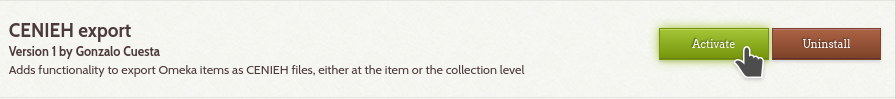
\includegraphics{../_static/images/plugins-act.png}
\caption{}\label{plugins-act}
}
\end{figure}

\begin{figure}
\hypertarget{plugins-des}{%
\centering
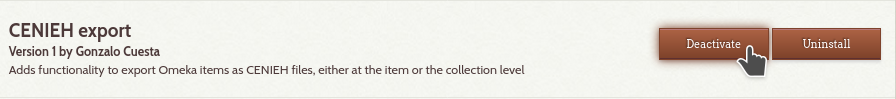
\includegraphics{../_static/images/plugins-des.png}
\caption{}\label{plugins-des}
}
\end{figure}

\hypertarget{desinstalar-complementos-plugins}{%
\paragraph{\texorpdfstring{Desinstalar complementos
(\emph{plugins})}{Desinstalar complementos (plugins)}}\label{desinstalar-complementos-plugins}}

Los complementos pueden ser desinstalados de la aplicación. Al
desinstalar un complemento o \emph{plugin} este puede volver a ser
instalado siempre y cuando conservemos los ficheros correspondientes en
la carpeta {/plugins} del directorio raíz de la aplicación.

Para desinstalar un complemento (\emph{plugin}):

\begin{enumerate}
\def\labelenumi{\arabic{enumi}.}
\tightlist
\item
  Desde el gestor de \emph{plugins} ({/admin/plugins}).
\item
  Localizar el nombre del complemento que se desea desinstalar.
\item
  Hacer clic sobre el botón "\emph{Uninstall}".
\end{enumerate}

\begin{figure}
\hypertarget{plugins-uninst-1}{%
\centering
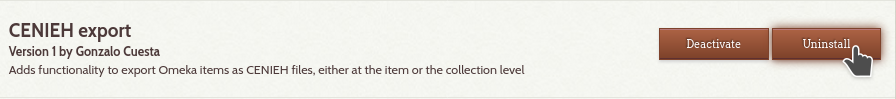
\includegraphics{../_static/images/plugins-uninst-1.png}
\caption{}\label{plugins-uninst-1}
}
\end{figure}

\begin{enumerate}
\def\labelenumi{\arabic{enumi}.}
\setcounter{enumi}{3}
\tightlist
\item
  En la página actual ({/admin/plugins}), leer las consecuencias de la
  desinstalación y, en caso de estar conforme, marcar la casilla
  "\emph{Yes, I want to uninstall this plugin.}".
\end{enumerate}

\begin{figure}
\hypertarget{plugins-uninst-2}{%
\centering
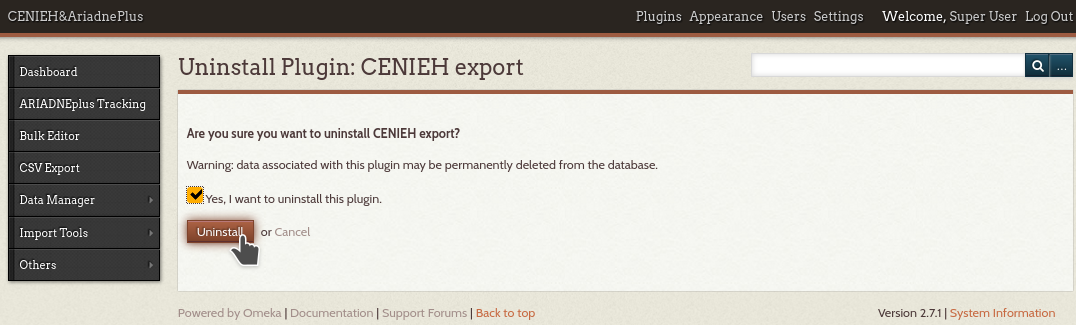
\includegraphics{../_static/images/plugins-uninst-2.png}
\caption{}\label{plugins-uninst-2}
}
\end{figure}

\begin{enumerate}
\def\labelenumi{\arabic{enumi}.}
\setcounter{enumi}{4}
\tightlist
\item
  Hacer clic sobre el botón rojo "\emph{Uninstall}".
\end{enumerate}

En caso de que deseemos realizar una \textbf{desinstalación completa},
es decir, eliminar por completo la extensión de la aplicación,
\textbf{despues de} ejecutar los pasos previamente mencionados, podemos
eliminar los ficheros asociados al \emph{plugin} de la carpeta
\emph{plugins} del directorio raíz de la aplicación.

\hypertarget{diseuxf1o-de-la-aplicaciuxf3n}{%
\subsubsection{Diseño de la
aplicación}\label{diseuxf1o-de-la-aplicaciuxf3n}}

Desde la entrada "\emph{Appearance}" del menú global podemos configurar
todos los aspectos de la aplicación relacionados con el diseño, que son:

\begin{figure}
\hypertarget{appearance}{%
\centering
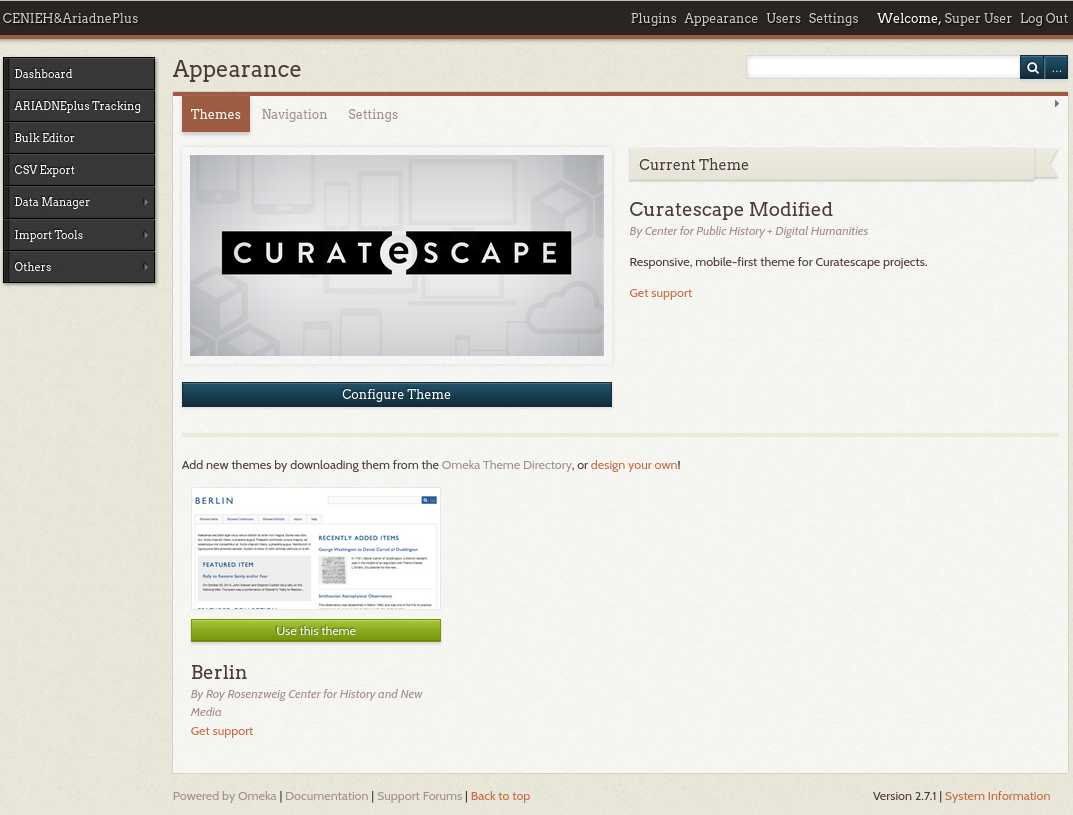
\includegraphics{../_static/images/appearance.png}
\caption{Vista principal de la página de configuración del diseño de la
aplicación}\label{appearance}
}
\end{figure}

\begin{itemize}
\tightlist
\item
  \emph{Themes}: permite seleccionar y configurar el tema público de la
  aplicación.
\item
  \emph{Navigation}: permite gestionar la navegación pública de la
  aplicación ordenando, editando y añadiendo nuevas entradas. Además se
  puede seleccionar la página principal (\emph{homepage}).
\item
  \emph{Settings}: permite configurar otros aspectos relacionados con el
  diseño de la aplicación.
\end{itemize}

\hypertarget{instalar-temas-themes}{%
\paragraph{\texorpdfstring{Instalar temas
(\emph{themes})}{Instalar temas (themes)}}\label{instalar-temas-themes}}

Warning

Si se siguieron a rajatabla los pasos de la
\protect\hyperlink{instalaciuxf3n}{Instalación}, la aplicación ya cuenta
el tema (\emph{theme}) propuesto dentro de la carpeta {/themes/}. Por lo
tanto, puedes saltarte el primer paso que ves a continuación e ir
directamente a los puntos de instalación. \textbf{El nombre del tema
propuesto es "Curatescape".}

El primer paso para instalar cualquier tema es descargarlo. Actualmente
existen dos sitios desde donde se pueden obtener temas (\emph{themes}):

\begin{enumerate}
\def\labelenumi{\arabic{enumi}.}
\tightlist
\item
  \href{https://omeka.org/classic/themes/}{Página oficial de Omeka}
\item
  \href{https://daniel-km.github.io/UpgradeToOmekaS/omeka_themes.html}{Repositorio
  de Github}
\end{enumerate}

Una vez descargado, se debe transportar la carpeta del tema
correspondiente a la carpeta {/themes/} del directorio raíz de la
aplicación.

Con el tema ya almacenado en la aplicación, se puede llevar a cabo el
proceso de instalación desde la plataforma.

Para instalar un tema (\emph{theme}):

\begin{enumerate}
\def\labelenumi{\arabic{enumi}.}
\tightlist
\item
  Desde la página de configuración de diseño ({/admin/appearance/}).
\item
  Hacer clic sobre la entrada "\emph{Themes}" de la barra de navegación
  existente.
\item
  Localizar el nombre del tema que se desea instalar.
\item
  Hacer clic sobre el botón "\emph{Use this theme}".
\end{enumerate}

\begin{figure}
\hypertarget{themes-inst}{%
\centering

\includegraphics{../_static/images/themes-inst.png}
\caption{}\label{themes-inst}
}
\end{figure}

\begin{enumerate}
\def\labelenumi{\arabic{enumi}.}
\setcounter{enumi}{4}
\tightlist
\item
  En caso de que el tema sea configurable, rellenar el formulario de
  configuración y hacer clic en el botón "\emph{Save Changes}".
\end{enumerate}

\hypertarget{modificar-la-navegaciuxf3n-puxfablica}{%
\paragraph{Modificar la navegación
pública}\label{modificar-la-navegaciuxf3n-puxfablica}}

Es posible modificar ciertos aspectos de la navegación pública de la
aplicación.

\begin{figure}
\hypertarget{nav-main}{%
\centering
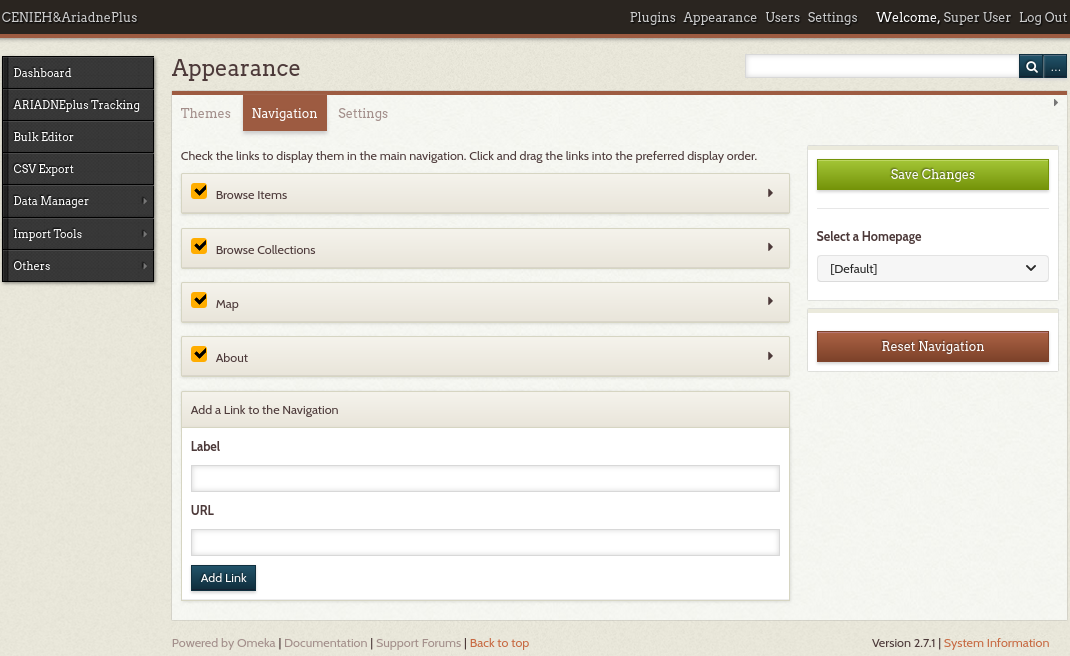
\includegraphics{../_static/images/nav-main.png}
\caption{Vista de la página de configuración de
navegación.}\label{nav-main}
}
\end{figure}

Para realizar cambios en la navegación pública de la aplicación:

\begin{enumerate}
\def\labelenumi{\arabic{enumi}.}
\tightlist
\item
  Desde la página de configuración de diseño ({/admin/appearance/}).
\item
  Hacer clic sobre la entrada "\emph{Navigation}" de la barra de
  navegación existente.
\item
  Realizar los cambios necesarios:

  \begin{enumerate}
  \def\labelenumii{\alph{enumii}.}
  \item
    Cambiar el orden de las entradas de navegación existentes.

    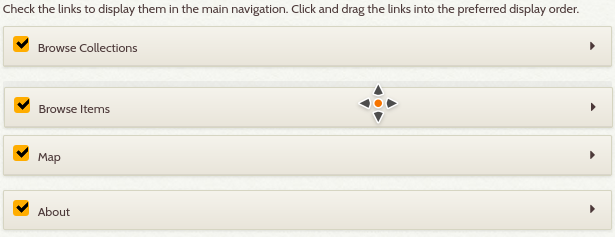
\includegraphics{../_static/images/nav-1.png}

    \begin{enumerate}
    \def\labelenumiii{\arabic{enumiii}.}
    \tightlist
    \item
      Seleccionar y desplazar la entrada a la posición deseada.
    \end{enumerate}
  \item
    Editar las entradas de navegación existentes.

    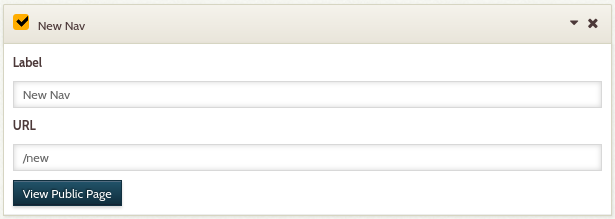
\includegraphics{../_static/images/nav-2.png}

    \begin{enumerate}
    \def\labelenumiii{\arabic{enumiii}.}
    \tightlist
    \item
      Clicar sobre la flecha situada en la parte derecha de la entrada.
    \item
      Realizar los cambios oportunos.
    \end{enumerate}
  \item
    Desactivar las entradas de navegación existentes.

    \begin{enumerate}
    \def\labelenumiii{\arabic{enumiii}.}
    \tightlist
    \item
      Desmarcar la casilla situada en la parte izquierda de la entrada
      correspondiente.
    \end{enumerate}
  \item
    Añadir nuevas entradas de navegación.

    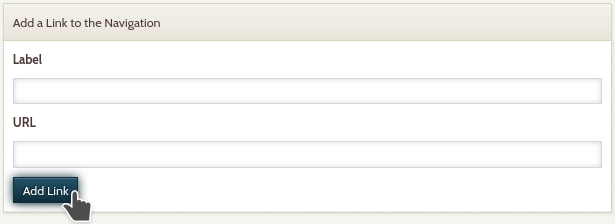
\includegraphics{../_static/images/nav-3.png}

    \begin{enumerate}
    \def\labelenumiii{\arabic{enumiii}.}
    \tightlist
    \item
      Introducir la etiqueta (\emph{label}) y el enlace (\emph{URL})
      correspondiente a la nueva entrada.
    \item
      Hacer clic sobre el botón "\emph{Add Link}".
    \end{enumerate}
  \item
    Establecer la página de inicio (\emph{homepage}).

    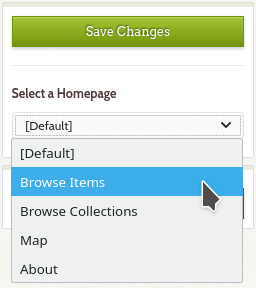
\includegraphics{../_static/images/nav-4.png}

    \begin{enumerate}
    \def\labelenumiii{\arabic{enumiii}.}
    \tightlist
    \item
      Seleccionar la entrada que deseamos establecer como
      \emph{homepage}.
    \end{enumerate}
  \item
    Resetear la configuración de navegación.

    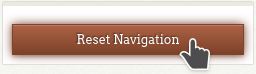
\includegraphics{../_static/images/nav-5.png}

    \begin{enumerate}
    \def\labelenumiii{\arabic{enumiii}.}
    \tightlist
    \item
      Hacer clic sobre el botón rojo "\emph{Reset Navigation}".
    \end{enumerate}
  \end{enumerate}
\item
  Hacer clic sobre el botón "\emph{Save changes}".
\end{enumerate}

\hypertarget{modificar-otros-aspectos-del-diseuxf1o-de-la-aplicaciuxf3n}{%
\paragraph{Modificar otros aspectos del diseño de la
aplicación}\label{modificar-otros-aspectos-del-diseuxf1o-de-la-aplicaciuxf3n}}

Existen ciertos aspectos del diseño de la aplicación que no están
ligados ni a los temas ni a la navegación.

\begin{figure}
\hypertarget{appearance-settings}{%
\centering
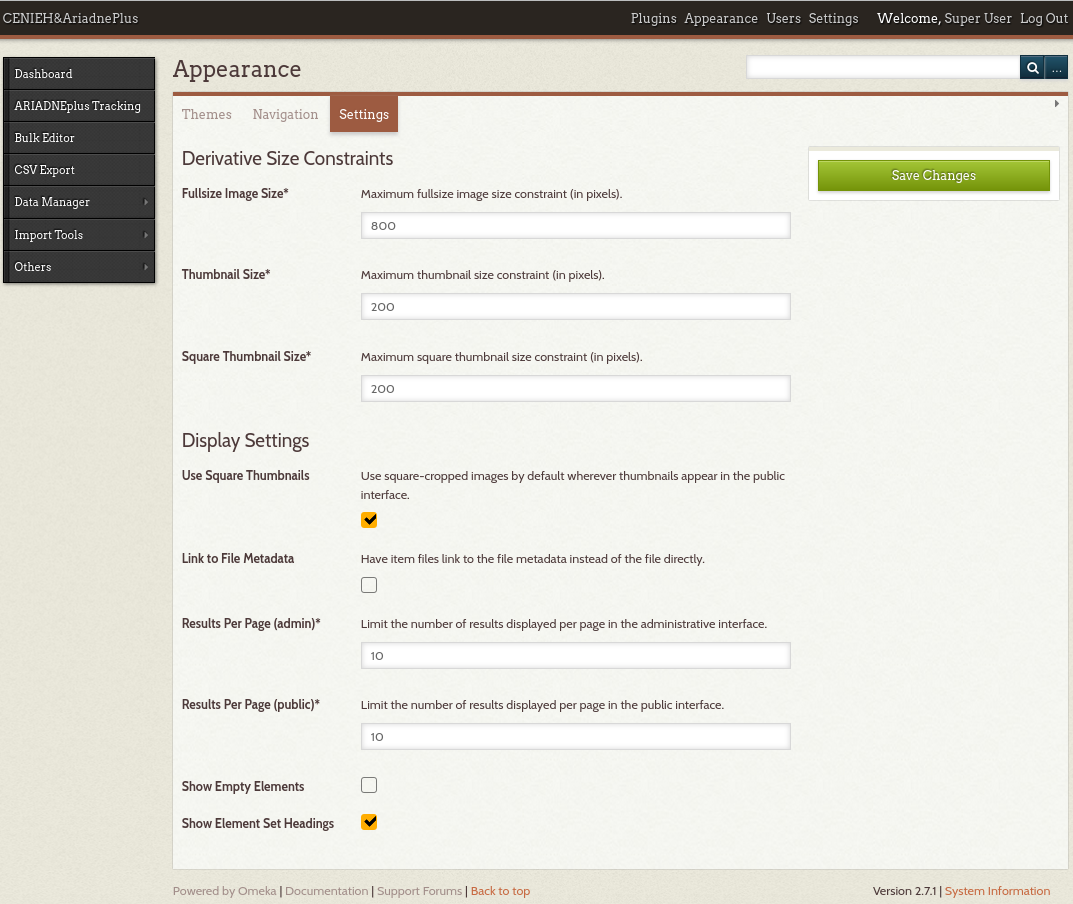
\includegraphics{../_static/images/appearance-settings.png}
\caption{Vista de la página de configuración de ciertos aspectos del
diseño de la aplicación}\label{appearance-settings}
}
\end{figure}

Para configurar estos aspectos:

\begin{enumerate}
\def\labelenumi{\arabic{enumi}.}
\tightlist
\item
  Desde la página de configuración de diseño ({/admin/appearance/}).
\item
  Hacer clic sobre la entrada "\emph{Settings}" de la barra de
  navegación existente.
\item
  Realizar los cambios oportunos:

  \begin{enumerate}
  \def\labelenumii{\alph{enumii}.}
  \tightlist
  \item
    \emph{Fullsize Image Size}: modificar el tamaño máximo de las
    imágenes.
  \item
    \emph{Thumbnail Size}: modificar el tamaño de las imágenes en
    miniatura.
  \item
    \emph{Thumbnail Size}: modificar el tamaño de las imágenes en
    miniatura cuadradas.
  \item
    \emph{Use Square Thumbnails}: usar imágenes en miniatura cuadradas
    para representar imágenes en la interfaz pública.
  \item
    \emph{Link to File Metadata}: cuando un ítem tenga un fichero
    asociado, enlazar el fichero con sus metadatos.
  \item
    \emph{Results Per Page (admin)}: modificar el número de ítems
    mostrados por página en el gestor de ítems.
  \item
    \emph{Results Per Page (public)}: modificar el número de ítems
    mostrados por página en el buscador de ítems (interfaz pública).
  \item
    \emph{Show Empty Elements}: mostrar metadatos vacíos.
  \item
    \emph{Show Element Set Headings}: mostrar el nombre del esquema de
    metadatos junto a sus elementos.
  \end{enumerate}
\item
  Hacer clic sobre el botón "\emph{Save changes}".
\end{enumerate}

\hypertarget{gestionar-usuarios}{%
\subsubsection{Gestionar Usuarios}\label{gestionar-usuarios}}

Para acceder al gestor de usuarios se utiliza la entrada "\emph{Users}"
del menú global de navegación.

\begin{figure}
\hypertarget{users}{%
\centering
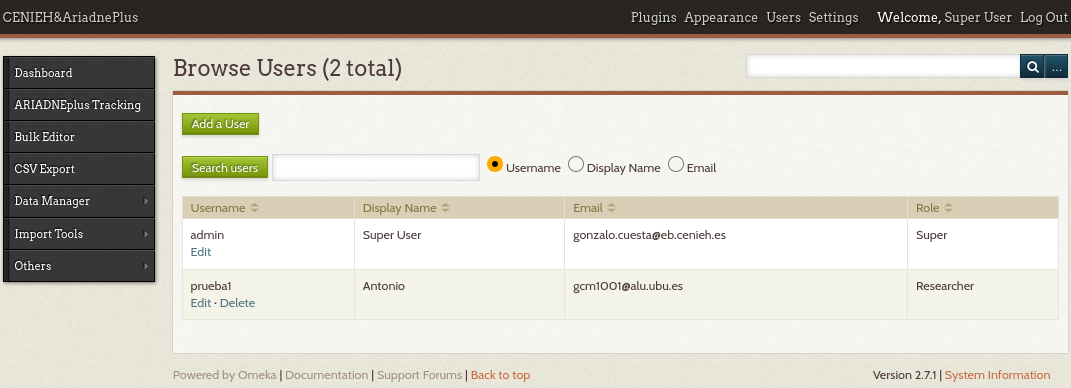
\includegraphics{../_static/images/users.png}
\caption{Vista principal del gestor de usuarios}\label{users}
}
\end{figure}

\hypertarget{crear-un-nuevo-usuario}{%
\paragraph{Crear un nuevo usuario}\label{crear-un-nuevo-usuario}}

Cuando se crea un usuario se envía un mensaje de confirmación al correo
electrónico indicado durante su creación. Este no será activado hasta
que se acceda al enlace de confirmación indicado en este mensaje. A
través de este enlace se accede a una página donde el usuario debe
establecer su contraseña.

Para crear un nuevo usuario:

\begin{enumerate}
\def\labelenumi{\arabic{enumi}.}
\item
  Desde el gestor de usuarios ({/admin/users}).
\item
  Hacer clic sobre el botón "\emph{Add user}" situado en la parte
  superior izquierda del gestor.
\item
  En la página actual, especificar:

  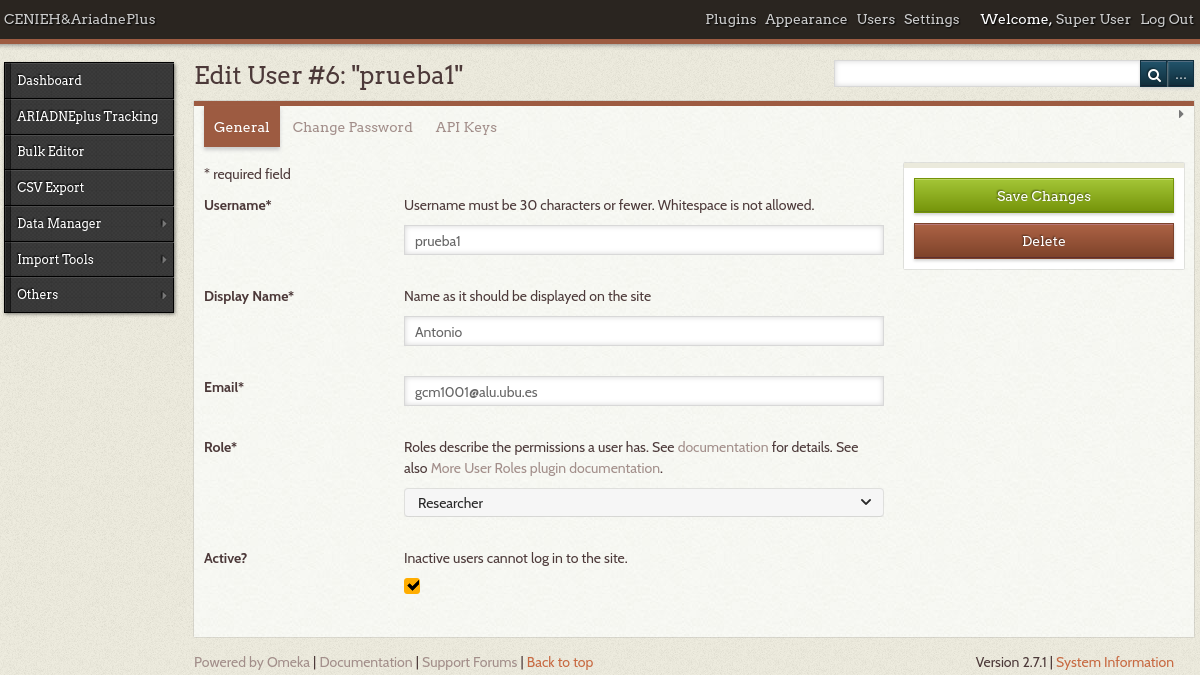
\includegraphics{../_static/images/new-user.png}

  3.1. \emph{Username}: nombre de usuario. 3.2. \emph{Display Name}:
  nombre que se mostrará a los demás usuarios. 3.3. \emph{Email}: correo
  electrónico. 3.4. \emph{Role}: rol de usuario. En función del rol un
  usuario cuenta con unos u otros permisos.
\item
  Hacer clic sobre el botón "\emph{Add User}" situado en la parte
  derecha de la pantalla.
\end{enumerate}

\hypertarget{eliminar-un-usuario}{%
\paragraph{Eliminar un usuario}\label{eliminar-un-usuario}}

Al eliminar un usuario, no se eliminan ninguno de los objetos digitales
(ítems, colecciones, \emph{tags}, etc.) creados por dicho usuario, sin
embargo, estos no podrán volver a ser asociados al usuario eliminado.

Para eliminar un usuario existente:

\begin{enumerate}
\def\labelenumi{\arabic{enumi}.}
\tightlist
\item
  Desde el gestor de usuarios ({/admin/users}).
\item
  Buscar en la tabla de usuarios el usuario que se pretende eliminar.
\item
  Una vez localizado, hacer clic sobre el hipertexto "\emph{Delete}"
  situado justo debajo del nombre de usuario.
\item
  Confirmar la eliminación haciendo clic sobre el botón rojo
  "\emph{Delete}".
\end{enumerate}

Warning

No es posible eliminar al usuario creado durante la instalación de la
aplicación.

\hypertarget{editar-un-usuario}{%
\paragraph{Editar un usuario}\label{editar-un-usuario}}

Todos los usuarios existentes en la plataforma pueden ser modificados.

Para editar un usuario existente:

\begin{enumerate}
\def\labelenumi{\arabic{enumi}.}
\item
  Desde el gestor de usuarios ({/admin/users}).
\item
  Buscar en la tabla de usuarios el usuario que se pretende editar.
\item
  Una vez localizado, hacer clic sobre el bipertexto "\emph{Edit}"
  situado justo debajo del nombre de usuario.
\item
  En la página actual
  ({mi/admin/users/edit/\textless idUser\textgreater{}}), realizar las
  modificaciones oportunas.

  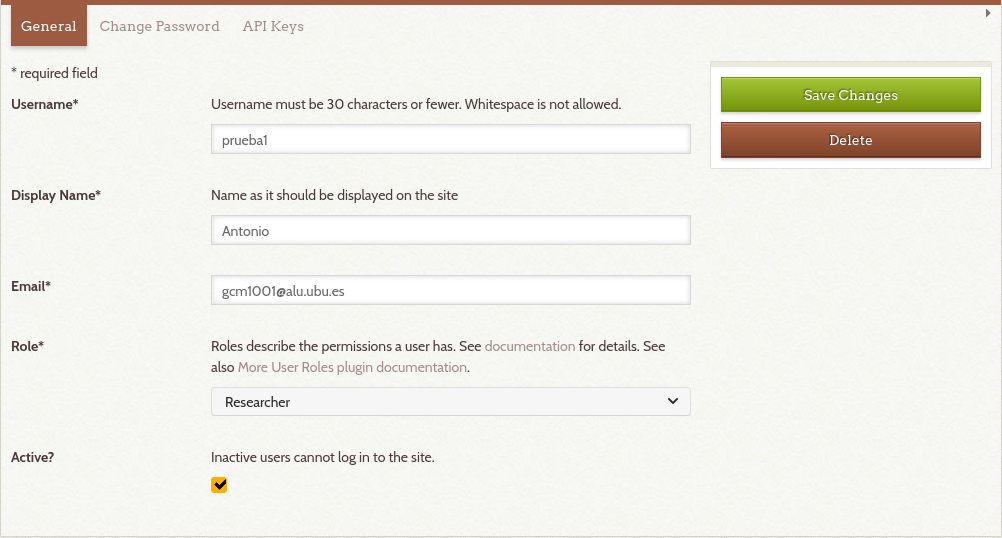
\includegraphics{../_static/images/user-mod-1.png}

  \begin{itemize}
  \tightlist
  \item
    \emph{Username}: cambiar el nombre de usuario.
  \item
    \emph{Display Name}: cambiar el nombre que se mostrará a los demás
    usuarios.
  \item
    \emph{Email}: cambiar el correo electrónico.
  \item
    \emph{Role}: cambiar el rol de usuario.
  \item
    \emph{Active?}: activar/desactivar el usuario.
  \end{itemize}

  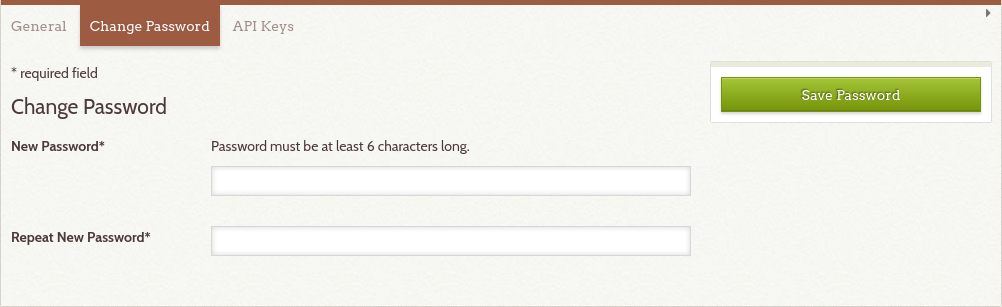
\includegraphics{../_static/images/user-mod-2.png}

  \begin{itemize}
  \tightlist
  \item
    Cambiar la contraseña.
  \end{itemize}

  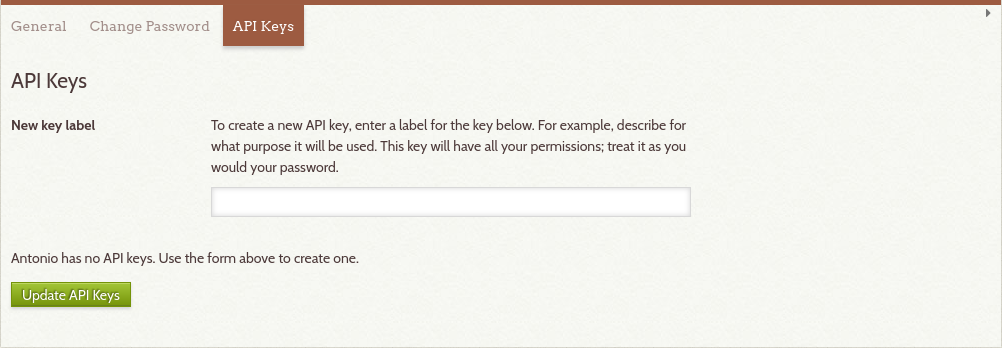
\includegraphics{../_static/images/user-mod-3.png}

  \begin{itemize}
  \tightlist
  \item
    Establecer/Cambiar la clave API.
  \end{itemize}
\end{enumerate}

\hypertarget{configuraciuxf3n-de-la-aplicaciuxf3n}{%
\subsubsection{Configuración de la
aplicación}\label{configuraciuxf3n-de-la-aplicaciuxf3n}}

Muchos de los elementos de la aplicación pueden ser configurados. Desde
la entrada "\emph{Settings}" del menú global se puede acceder a la
página desde donde se realizan estas configuraciones.

\begin{figure}
\hypertarget{settings}{%
\centering
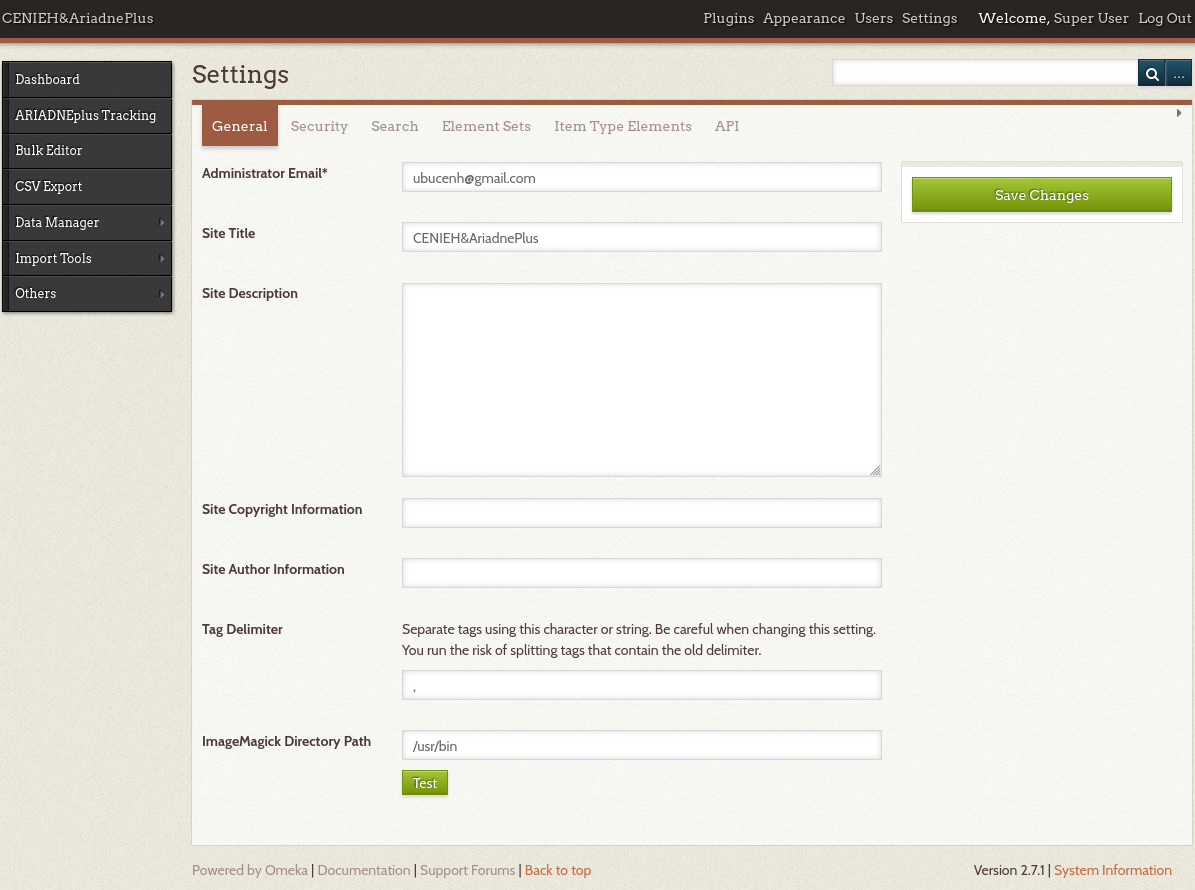
\includegraphics{../_static/images/settings.png}
\caption{Vista de la página de configuración principal de la
aplicación}\label{settings}
}
\end{figure}

A través de la barra de navegación podemos desplazarnos por las
distintas zonas de configuración, cada una de las cuales abarca un
aspecto determinado.

\hypertarget{configuraciuxf3n-general}{%
\paragraph{Configuración general}\label{configuraciuxf3n-general}}

Desde la pestaña "\emph{General}" de la barra de navegación existente en
la página de configuración principal de la aplicación
({mi/admin/settings/}), se pueden llevan a cabo las siguientes
configuraciones:

\begin{figure}
\hypertarget{settings-general}{%
\centering
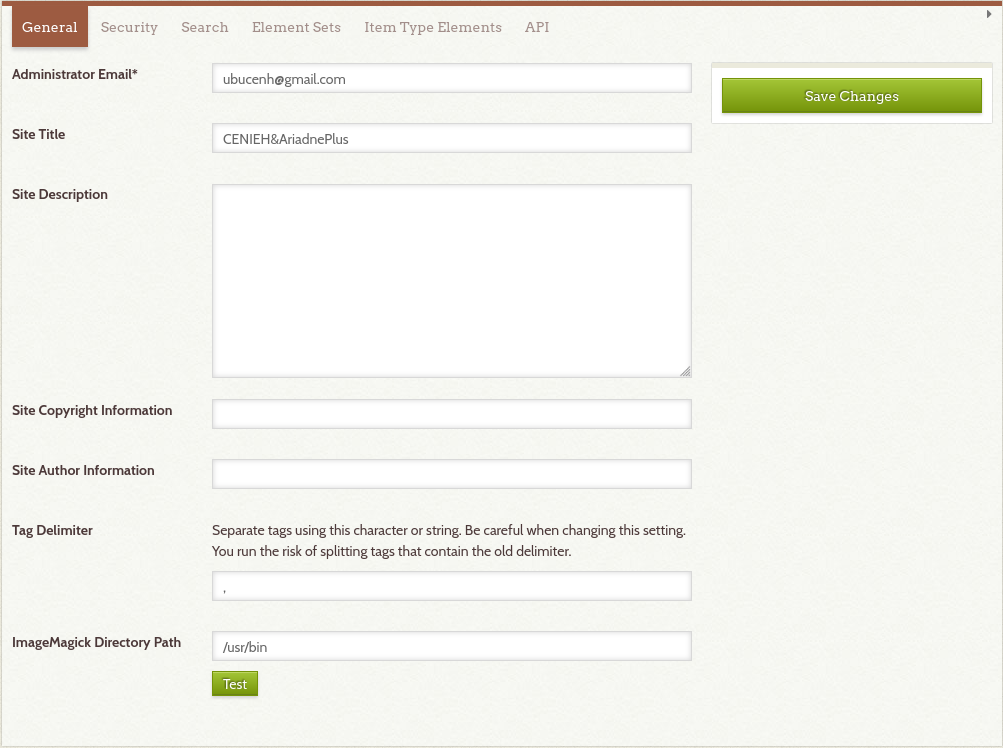
\includegraphics{../_static/images/settings-general.png}
\caption{Vista de la página de configuración principal de la aplicación,
apartado "General".}\label{settings-general}
}
\end{figure}

\begin{itemize}
\tightlist
\item
  \emph{Administrator Email}: email de administración.
\item
  \emph{Site Title}: título del sitio.
\item
  \emph{Site Description}: descripción del sitio:
\item
  \emph{Site Copyright Information}: información de \emph{copyright} del
  sitio.
\item
  \emph{Site Author Information}: información del autor del sitio.
\item
  \emph{Tag Delimiter}: caracter usado para delimitar los \emph{tags} de
  la aplicación.
\item
  \emph{ImageMagick Directory Path}: directorio donde se encuentra
  instalada la aplicación \emph{ImageMagick}.
\end{itemize}

\hypertarget{configuraciuxf3n-de-la-seguridad}{%
\paragraph{Configuración de la
seguridad}\label{configuraciuxf3n-de-la-seguridad}}

Desde la pestaña "\emph{Security}" de la barra de navegación existente
en la página de configuración principal de la aplicación
({mi/admin/settings/}), se pueden llevan a cabo las siguientes
configuraciones:

\begin{itemize}
\item
  \emph{File Validation}: configuraciones relacionadas con la validación
  de ficheros.

  \begin{quote}
  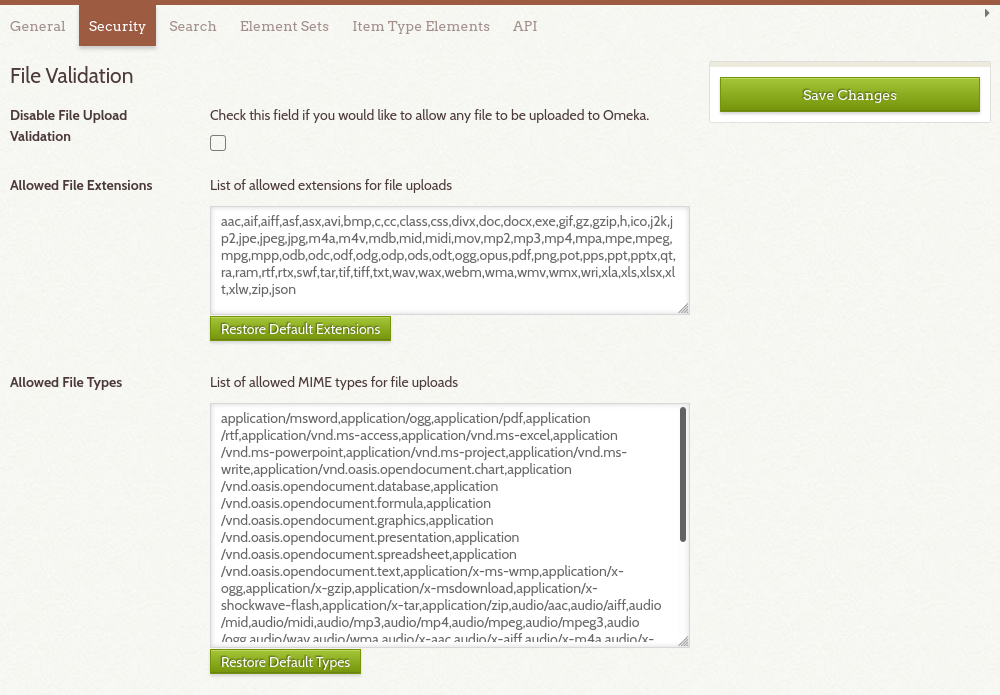
\includegraphics{../_static/images/sec-1.png}

  \begin{itemize}
  \tightlist
  \item
    \emph{Disable File Upload Validation}: desactivar/activar la
    validación de ficheros (se permite cualquier entrada de ficheros).
  \item
    \emph{Allowed File Extensions}: extensiones de ficheros permitidas.
  \item
    \emph{Allowed File Types}: tipos (\emph{MIME Types}) de ficheros
    permitidos.
  \end{itemize}
  \end{quote}
\item
  \emph{Captcha}: configuraciones relacionadas con el sistema
  \emph{Captcha}.

  \begin{quote}
  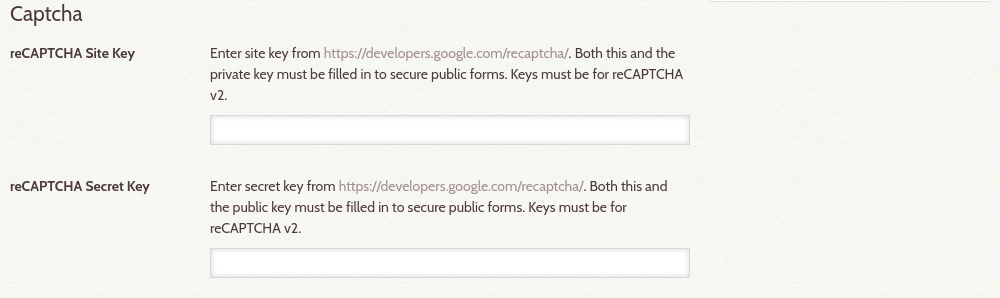
\includegraphics{../_static/images/sec-2.png}

  \begin{itemize}
  \tightlist
  \item
    \emph{reCAPTCHA Site Key}: establecer la clave del sitio utilizada
    por el sistema \emph{Captcha}.
  \item
    \emph{reCAPTCHA Secret Key}: establecer la clave secreta utilizada
    por el sistema \emph{Captcha}.
  \end{itemize}
  \end{quote}
\item
  \emph{HTML Filtering}: configuraciones relacionadas con el filtro
  HTML.

  \begin{quote}
  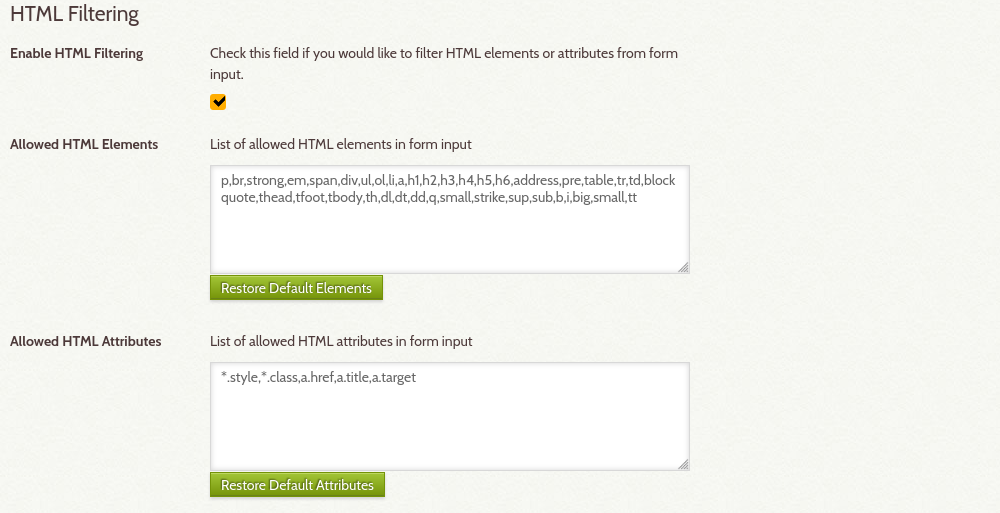
\includegraphics{../_static/images/sec-3.png}

  \begin{itemize}
  \tightlist
  \item
    \emph{Enable HTML Filtering}: activar/desactivar el filtro HTML.
  \item
    \emph{Allowed HTML Elements}: indicar que elementos HTML pueden
    pasar el filtro HTML.
  \item
    \emph{Allowed HTML Attributes}: indicar que atributos HTML pueden
    pasar el filtro HTML.
  \end{itemize}
  \end{quote}
\end{itemize}

\hypertarget{configuraciuxf3n-de-las-buxfasquedas}{%
\paragraph{Configuración de las
búsquedas}\label{configuraciuxf3n-de-las-buxfasquedas}}

Desde la pestaña "\emph{Search}" de la barra de navegación existente en
la página de configuración principal de la aplicación
({mi/admin/settings/}), se pueden llevan a cabo las siguientes
configuraciones:

\begin{figure}
\hypertarget{settings-search}{%
\centering
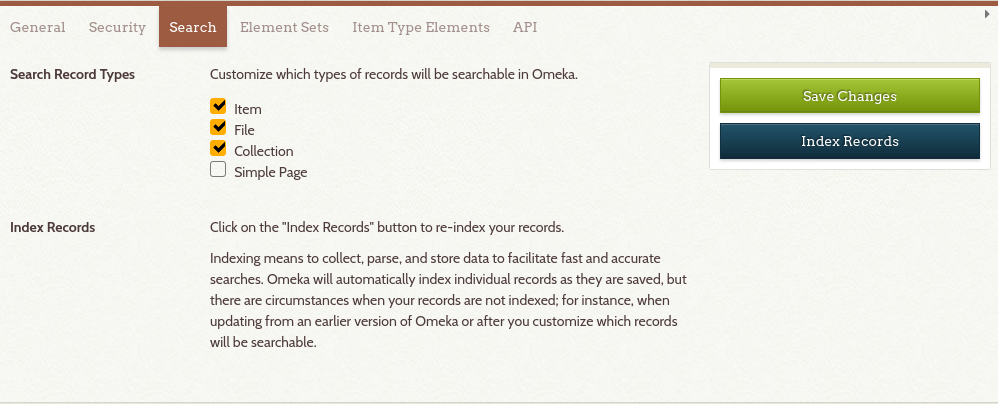
\includegraphics{../_static/images/settings-search.png}
\caption{Vista de la página de configuración principal de la aplicación,
apartado "Search".}\label{settings-search}
}
\end{figure}

\begin{itemize}
\tightlist
\item
  \emph{Search Record Types}: seleccionar que objetos digitales pueden
  ser buscados desde la aplicación.
\item
  \emph{Index Records}: clicar sobre el botón "\emph{Index Records}" si
  se desea re-indexar todos los objetos digitales.
\end{itemize}

\hypertarget{configuraciuxf3n-de-los-esquemas-de-metadatos}{%
\paragraph{Configuración de los esquemas de
metadatos}\label{configuraciuxf3n-de-los-esquemas-de-metadatos}}

Desde la pestaña "\emph{Element Sets}" de la barra de navegación
existente en la página de configuración principal de la aplicación
({mi/admin/settings/}), se pueden llevan a cabo las siguientes
configuraciones:

\begin{figure}
\hypertarget{settings-es}{%
\centering
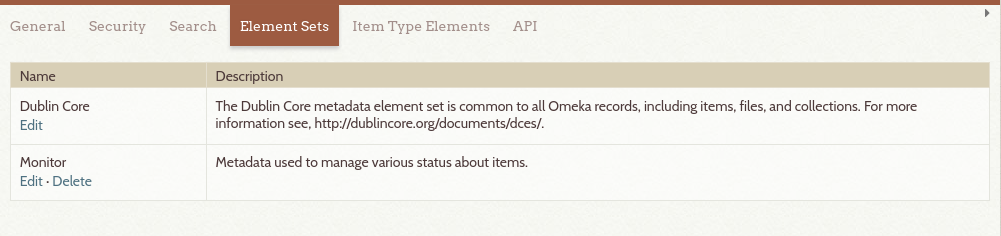
\includegraphics{../_static/images/settings-es.png}
\caption{Vista de la página de configuración principal de la aplicación,
apartado "Element Sets".}\label{settings-es}
}
\end{figure}

\begin{itemize}
\tightlist
\item
  \emph{Edit}: editar el esquema de metadatos.
\item
  \emph{Delete}: eliminar el esque de metadatos.
\end{itemize}

\hypertarget{configuraciuxf3n-de-los-metadatos-usados-en-los-tipos-de-uxedtem}{%
\paragraph{Configuración de los metadatos usados en los tipos de
ítem}\label{configuraciuxf3n-de-los-metadatos-usados-en-los-tipos-de-uxedtem}}

Desde la pestaña "\emph{Item Type Elements}" de la barra de navegación
existente en la página de configuración principal de la aplicación
({mi/admin/settings/}), se pueden llevan a cabo las siguientes
configuraciones:

\begin{figure}
\hypertarget{settings-it}{%
\centering
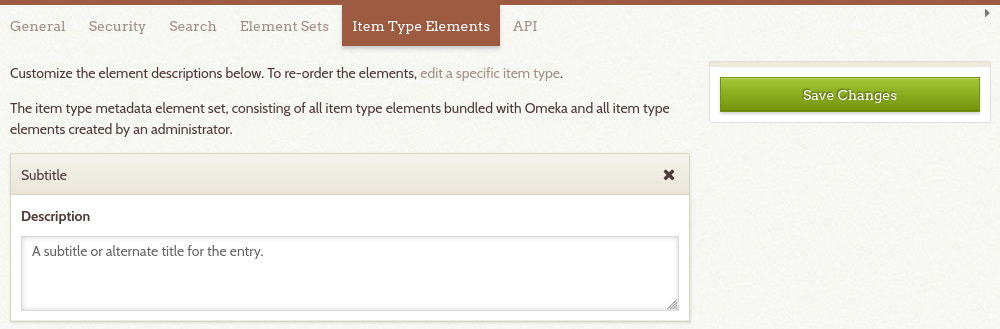
\includegraphics{../_static/images/settings-it.png}
\caption{Vista de la página de configuración principal de la aplicación,
pestaña "Item Type Elements".}\label{settings-it}
}
\end{figure}

\begin{itemize}
\tightlist
\item
  \emph{x}: eliminar el elemento (metadato) del esquema de metadatos
  utilizado por los tipos de ítem.
\item
  \emph{Description}: modificar/añadir una descripción al elemento
  (metadato) del esquema de metadatos utilizado por los tipos de ítem.
\end{itemize}

\hypertarget{configuraciuxf3n-de-la-api}{%
\paragraph{Configuración de la API}\label{configuraciuxf3n-de-la-api}}

Desde la pestaña "\emph{API}" de la barra de navegación existente en la
página de configuración principal de la aplicación
({mi/admin/settings/}), se pueden llevan a cabo las siguientes
configuraciones:

\begin{figure}
\hypertarget{settings-api}{%
\centering
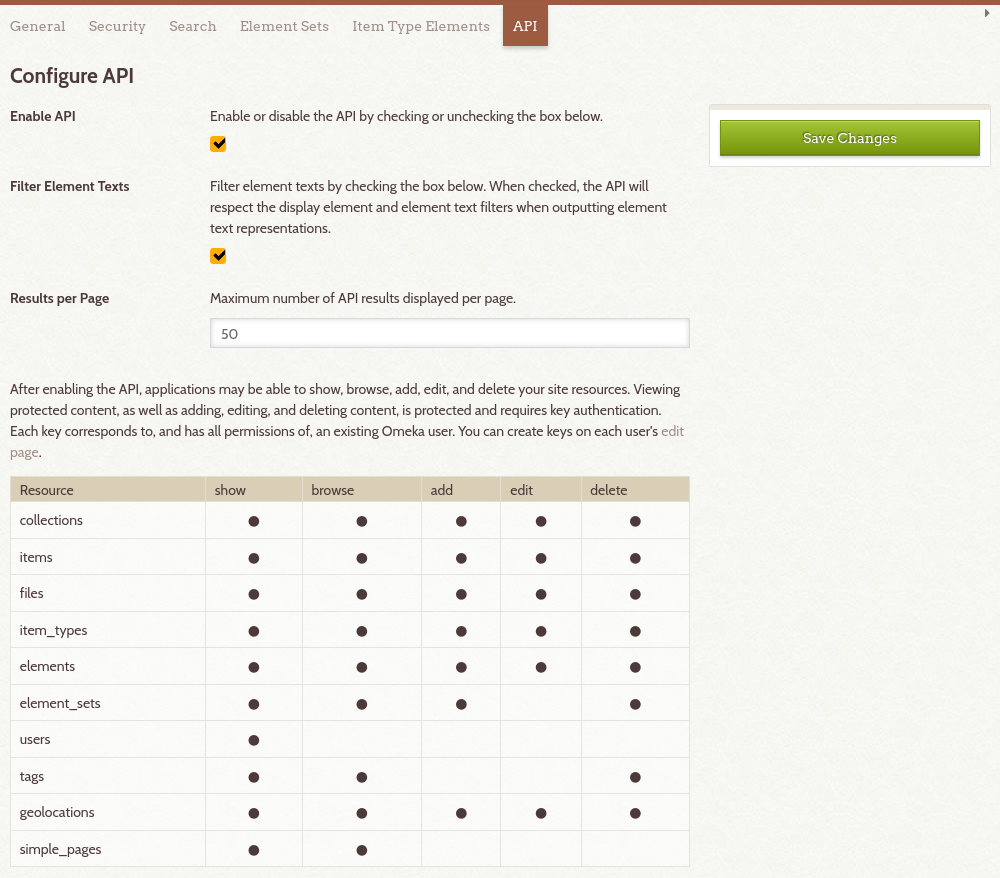
\includegraphics{../_static/images/settings-api.png}
\caption{Vista de la página de configuración principal de la aplicación,
pestaña "API".}\label{settings-api}
}
\end{figure}

\begin{itemize}
\tightlist
\item
  \emph{Enable API}: activar/desactivar la API.
\item
  \emph{Filter Element Texts}: activar/desactivar el filtro de esquemas
  de metadatos.
\item
  \emph{Results per Page}: establecer el número máximo de resultados por
  página.
\end{itemize}

\hypertarget{objetos-digitales}{%
\subsection{Objetos digitales}\label{objetos-digitales}}

Dentro de la aplicación nos podemos encontrar con cinco tipos de objetos
digitales: \textbf{ítems} (\emph{Items}), \textbf{colecciones}
(\emph{Collections}), \textbf{etiquetas} (\emph{Tags}),
\textbf{ficheros} (\emph{Files}) y \textbf{tipos de ítem} (\emph{Item
Types}). En este apartado se explica la utilidad de cada uno de ellos y,
además, se muestran algunos tutoriales de cómo gestionar estos objetos
dentro de la aplicación.

\hypertarget{items}{%
\subsubsection{\texorpdfstring{\emph{Items}}{Items}}\label{items}}

Los ítems son los \textbf{elementos principales} de la aplicación,
utilizados para representar a cada uno de los objetos digitales
almacenados en esta. A través de la entrada \emph{Items}, dentro de la
sección "\emph{Data Manager}" del menú principal, se accede al gestor de
ítems ({/admin/items/}), lugar donde se llevan a cabo todas las tareas
de gestión relacionadas con este elemento.

\begin{figure}
\hypertarget{items-view}{%
\centering
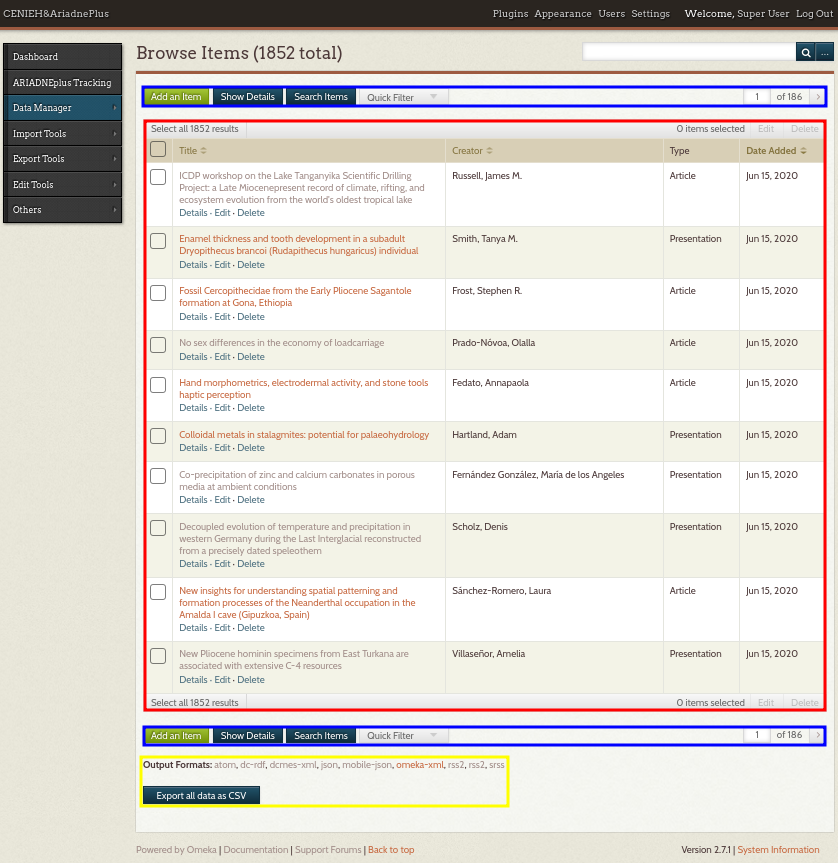
\includegraphics{../_static/images/items-view.png}
\caption{Vista principal del gestor de ítems}\label{items-view}
}
\end{figure}

\hypertarget{propiedades-de-un-item}{%
\paragraph{\texorpdfstring{Propiedades de un
\emph{Item}}{Propiedades de un Item}}\label{propiedades-de-un-item}}

Cada \emph{Item} está formado por:

\begin{itemize}
\tightlist
\item
  0 o más elementos de información (metadatos).
\item
  0 o más ficheros (\emph{Files}).
\item
  0 o más etiquetas (\emph{Tags}).
\item
  0 o 1 geolocalización (\emph{Geolocation}).
\end{itemize}

Además, presenta tres valores especiales:

\begin{itemize}
\tightlist
\item
  \emph{Public}: indica si el ítem es público o no.
\item
  \emph{Feature}: indica si el ítem será destacado o no.
\item
  \emph{Collection}: indica si el ítem pertenece a una colección de
  ítems.
\end{itemize}

\hypertarget{crear-un-uxedtem}{%
\paragraph{Crear un ítem}\label{crear-un-uxedtem}}

Si se desean generar conjuntos de datos desde la aplicación, el primer
paso es crear ítems.

\begin{figure}
\hypertarget{add-items-view}{%
\centering
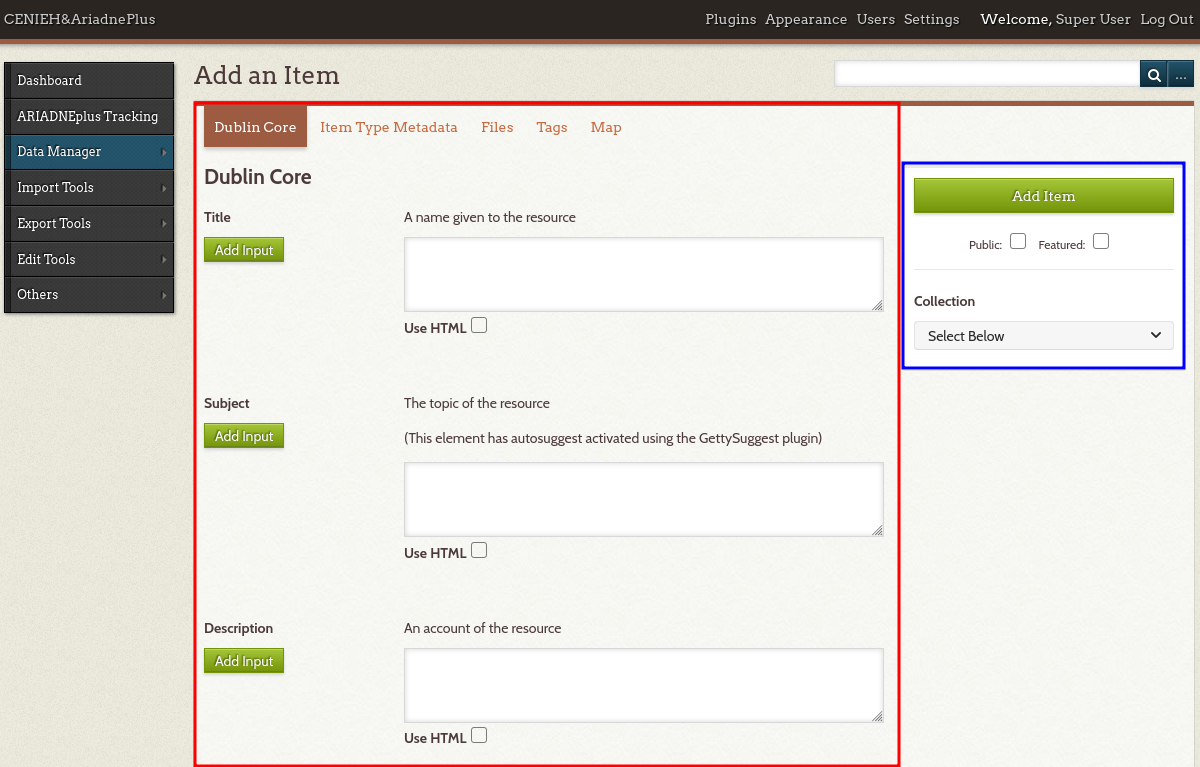
\includegraphics{../_static/images/add-items-view.png}
\caption{Vista utilizada para la creación de
ítems}\label{add-items-view}
}
\end{figure}

Para crear un ítem:

\begin{enumerate}
\def\labelenumi{\arabic{enumi}.}
\tightlist
\item
  Desde el gestor de ítems ({/admin/items/}).
\item
  Hacer clic sobre el botón "\emph{Add an Item}" situado en la parte
  superior de la tabla (ver \texttt{items-view}).
\item
  En la página actual ({/admin/items/add}), se puede observar una barra
  de navegación (ver \texttt{add-items-view}). Desde ella se pueden
  configurar los elementos del ítem:

  \begin{enumerate}
  \def\labelenumii{\alph{enumii}.}
  \tightlist
  \item
    \emph{Dublin Core}: metadatos del esquema de metadatos \emph{Dublin
    Core}.
  \item
    \emph{Item Type Metadata}: metadatos asociados al tipo de
    \emph{Item}.
  \item
    \emph{Files}: ficheros asociados.
  \item
    \emph{Tags}: etiquetas asociadas.
  \item
    \emph{Map}: geolocalización del ítem.
  \end{enumerate}
\item
  Si queremos asignar el ítem a una colección:

  \begin{enumerate}
  \def\labelenumii{\alph{enumii}.}
  \tightlist
  \item
    En la parte derecha de la página, debajo del botón "\emph{Add
    Item}", hay un menú desplegable donde puede asignar el ítem actual a
    la colección seleccionada.
  \end{enumerate}
\item
  Además, se pueden marcar las casillas "\emph{Public}" y/o
  "\emph{Feature}" en la parte derecha del formulario, justo debajo del
  botón "\emph{Add Item}".
\item
  Para finalizar, hacer clic sobre el botón "\emph{Add Item}".
\end{enumerate}

\hypertarget{editar-un-uxedtem}{%
\paragraph{Editar un ítem}\label{editar-un-uxedtem}}

Existen numerosos motivos por los que pueden surgir la necesidad de
editar un ítem como, por ejemplo, cambiar el contenido de sus
metadatados, agregar/eliminar ficheros, agruparlo a una colección,
publicarlo, etc.

\begin{figure}
\hypertarget{edit-items-view}{%
\centering
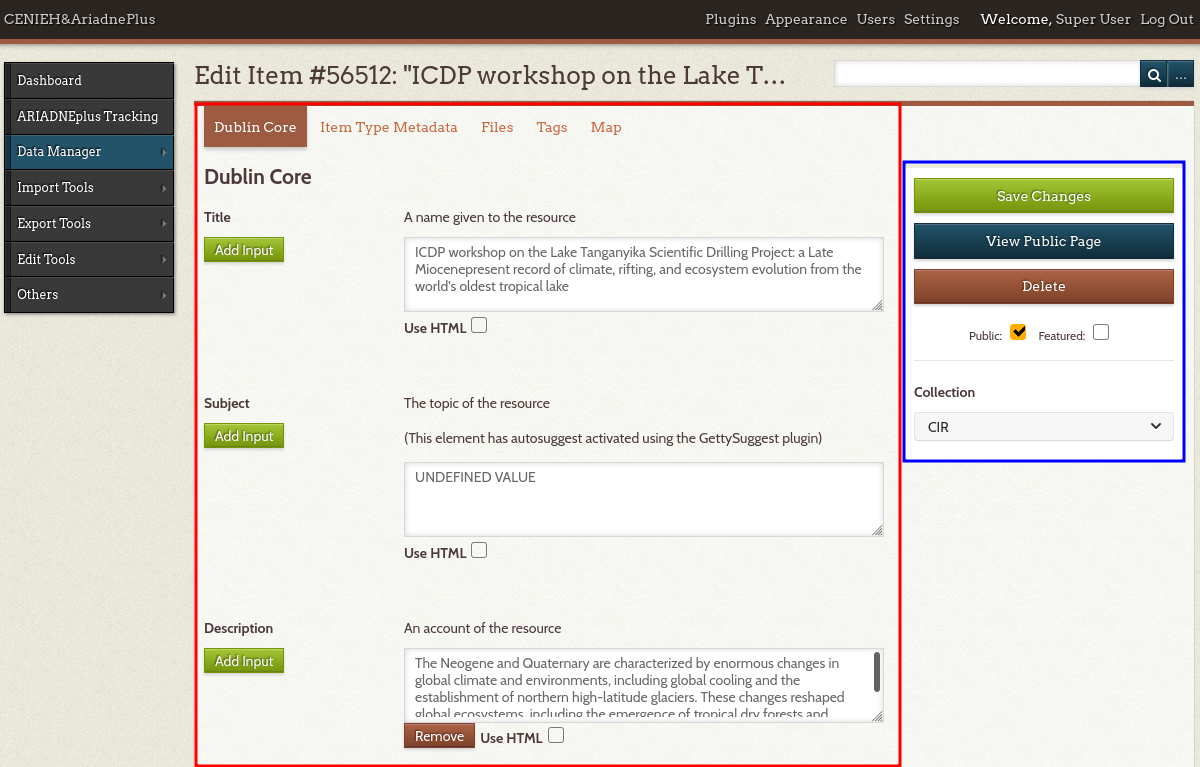
\includegraphics{../_static/images/edit-items-view.png}
\caption{Vista utilizada para la edición de
ítems}\label{edit-items-view}
}
\end{figure}

Para editar un ítem existente:

\begin{enumerate}
\def\labelenumi{\arabic{enumi}.}
\tightlist
\item
  Desde el gestor de ítems ({/admin/items/}).
\item
  Localizar la fila en la que se encuentra el ítem y hacer clic sobre el
  hipertexto "\emph{Edit}" situado justo debajo del título del ítem (ver
  \texttt{items-view}).
\item
  En la página actual
  ({/admin/item/edit/\textless itemid\textgreater{}}), se puede observar
  una barra de navegación (ver \texttt{edit-items-view}). Desde ella se
  pueden configurar los elementos del ítem:

  \begin{enumerate}
  \def\labelenumii{\alph{enumii}.}
  \tightlist
  \item
    \emph{Dublin Core}: metadatos del esquema de metadatos \emph{Dublin
    Core}.
  \item
    \emph{Item Type Metadata}: metadatos asociados al tipo de ítem.
  \item
    \emph{Files}: ficheros asociados.
  \item
    \emph{Tags}: etiquetas asociadas.
  \item
    \emph{Map}: geolocalización del ítem.
  \end{enumerate}
\item
  Asignar el ítem a una colección:

  \begin{enumerate}
  \def\labelenumii{\alph{enumii}.}
  \tightlist
  \item
    En la parte derecha de la página, debajo del botón "\emph{Add
    Item}", hay un menú desplegable donde puede asignar el ítem actual a
    la colección seleccionada.
  \end{enumerate}
\item
  Además, se pueden marcar las casillas "\emph{Public}" y/o
  "\emph{Feature}" situadas en la parte derecha del formulario, justo
  debajo del botón "\emph{Add Item}".

  \begin{enumerate}
  \def\labelenumii{\alph{enumii}.}
  \tightlist
  \item
    \emph{Public} para publicar el ítem.
  \item
    \emph{Feature} para destacar el ítem.
  \end{enumerate}
\item
  Para finalizar, hacer clic sobre el botón "\emph{Save Changes}".
\end{enumerate}

\hypertarget{eliminar-un-uxedtem}{%
\paragraph{Eliminar un ítem}\label{eliminar-un-uxedtem}}

El gestor de ítems ofrece múltiples formas de eliminar un ítem existente
en la plataforma.

\emph{{[}Opción 1{]}} Para eliminar un ítem existente:

\begin{enumerate}
\def\labelenumi{\arabic{enumi}.}
\tightlist
\item
  Desde el gestor de ítems ({/admin/items/}).
\item
  Localizar la fila en la que se encuentra el ítem y hacer clic sobre el
  hipertexto "\emph{Delete}" situado justo debajo del título del ítem.
\item
  Confirmar la eliminación del ítem pulsando sobre el botón
  "\emph{Delete}".
\end{enumerate}

\emph{{[}Opción 2{]}} Para eliminar un ítem existente:

\begin{enumerate}
\def\labelenumi{\arabic{enumi}.}
\tightlist
\item
  Desde el gestor de ítems ({/admin/items/}).
\item
  Localizar la fila en la que se encuentra el ítem y hacer clic sobre el
  hipertexto "\emph{Edit}" situado justo debajo del título del ítem.
\item
  En la página actual
  ({/admin/item/edit/\textless itemid\textgreater{}}), clicar sobre el
  botón "\emph{Delete}" situado en la parte derecha del formulario.
\item
  Confirmar la eliminación del ítem pulsando sobre el botón
  "\emph{Delete}".
\end{enumerate}

\emph{{[}Opción 3{]}} Para eliminar un ítem existente:

\begin{enumerate}
\def\labelenumi{\arabic{enumi}.}
\tightlist
\item
  Desde el gestor de ítems ({/admin/items/}).
\item
  Localizar la fila en la que se encuentra el ítem y hacer clic sobre la
  casilla situada en la primera columna de la izquierda de la tabla.
\item
  Hacer clic sobre el botón "\emph{Delete}" situado en la parte superior
  derecha de la tabla.
\item
  En la página actual ({/admin/items/batch-edit}), hacer clic sobre el
  botón "\emph{Delete Items}" situado en la parte derecha de la página.
\end{enumerate}

\hypertarget{buscar-uxedtems}{%
\paragraph{Buscar ítems}\label{buscar-uxedtems}}

Otro de los servicios que incluye este gestor es la búsqueda de ítems.
Cuando entramos a este apartado a través de la sección "\emph{Data
Manager}" del menú principal, se nos muestra una lista de ítems
ordenados según su fecha de creación (de más recientes a más antiguos).

Como se puede apreciar en la \texttt{items-view}, los ítems son
mostrados en una tabla donde cada fila representa a un ítem y cada
columna contiene información específica de dicho ítem (título, creador,
tipo de ítem y fecha de creación). Existe una columna adicional, en la
parte izquierda de la tabla, que se utiliza para seleccionar varios
ítems en el caso de que se quieran ejecutar una o varias acciones sobre
varios ítems. Para ordenar los ítems en funcion de los campos de la
tabla (título, creador y fecha de modificación), se debe clicar sobre el
elemento deseado.

\begin{figure}
\hypertarget{special-items-view}{%
\centering
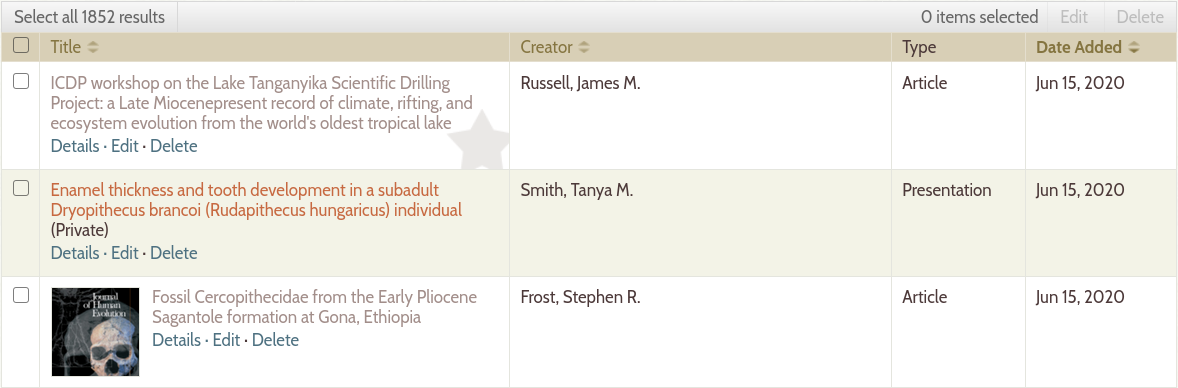
\includegraphics{../_static/images/special-items.png}
\caption{Ítems especiales vistos desde el gestor de ítems: el primero es
destacado, el segundo es privado y el tercero almacena un fichero
(imagen)}\label{special-items-view}
}
\end{figure}

Otra particularidad del gestor es que, en función de los valores
especiales del ítem, se le da un formato u otro.

\begin{itemize}
\tightlist
\item
  Si al lado del título se encuentra el texto "(\emph{Private})" , el
  ítem no es público, es decir, solo será accesible desde la zona de
  administración.
\item
  Si el fondo del título presenta una estrella, significa que el ítem es
  destacado (\emph{feature}).
\item
  Si el ítem tiene un archivo (\emph{File}) asociado, se mostrará una
  miniatura del misma al lado del título.
\end{itemize}

Por defecto se muestran todos los ítems almacenados en la plataforma,
sin embargo, es posible reducir su número ejecutando una búsqueda
avanzada o aplicando filtros. De esta manera, se pueden enfocar las
labores de gestión sobre unos ítems específicos.

Para buscar ítems mediante una búsqueda avanzada:

\begin{enumerate}
\def\labelenumi{\arabic{enumi}.}
\item
  Desde el gestor de ítems ({/admin/items/}).
\item
  Hacer clic sobre el botón "\emph{Search items}" situado justo
  encima/debajo de la tabla de ítems.
\item
  En la página actual ({/admin/items/search}), rellenar el formulario
  con los datos de búsqueda.

  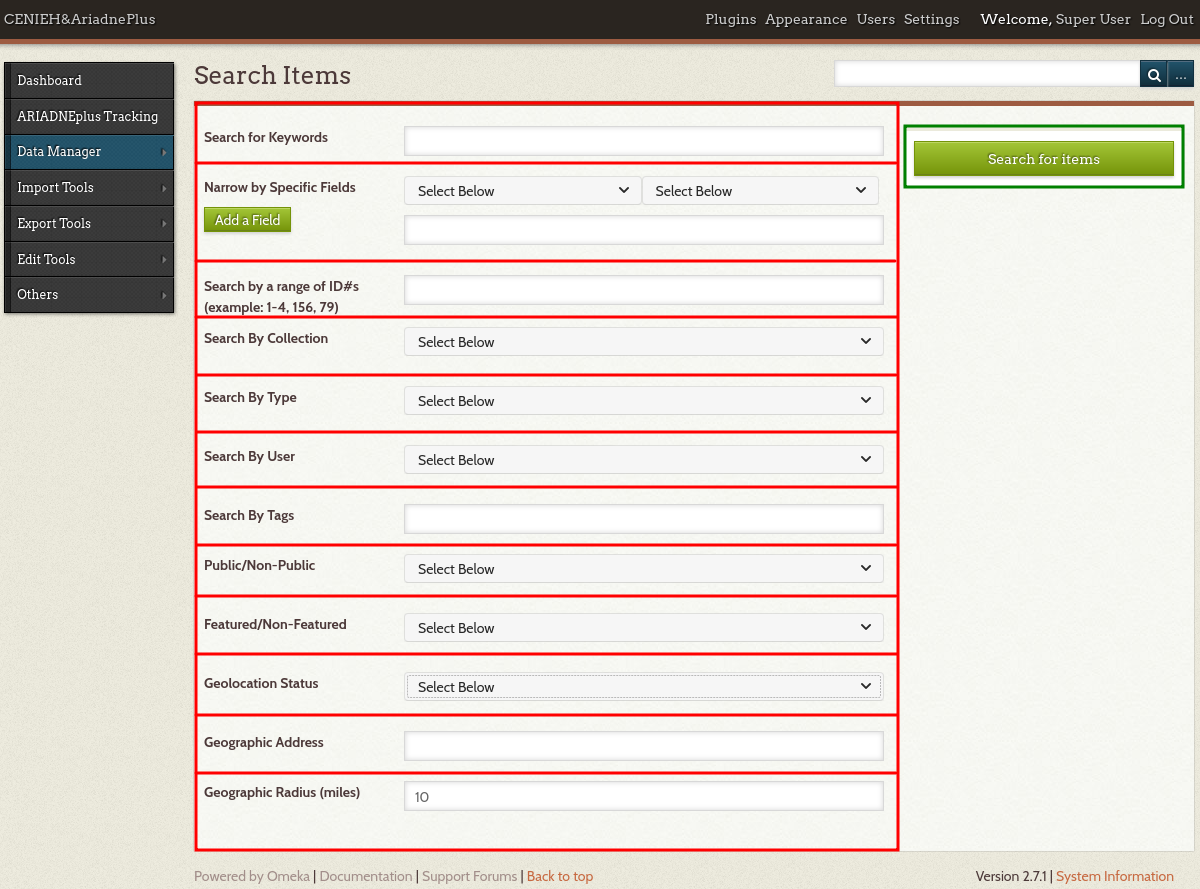
\includegraphics{../_static/images/advanced-search.png}

  \begin{enumerate}
  \def\labelenumii{\alph{enumii}.}
  \tightlist
  \item
    \emph{Search for Keywords}: buscar por una cadena de texto
    específica (en cualquier elemento).
  \item
    \emph{Narrow by Specific Fields}: buscar por un elemento (metadato)
    específico que..

    \begin{itemize}
    \tightlist
    \item
      \emph{contains}: contenga una cadena de texto
    \item
      \emph{does not contain}: no contenga una cadena de texto
    \item
      \emph{is exactly}: sea exactamente una cadena de texto
    \item
      \emph{is not exactly}: no sea exactamente una cadena de texto
    \item
      \emph{is empty}: esté vacío
    \item
      \emph{is not empty}: no esté vacío
    \item
      \emph{starts with}: empiece por una cadena de texto
    \item
      \emph{ends with}: acabe por una cadena de texto
    \item
      \emph{matches}: coincida con una expresión
    \item
      \emph{does not match}: no coincida con una expresión
    \end{itemize}
  \item
    \emph{Search by a range of ID}: buscar por rangos de
    identificadores.
  \item
    \emph{Search By Collection}: buscar por colección asociada.
  \item
    \emph{Search By User}: buscar por el usuario que lo creó/importó.
  \item
    \emph{Search By Tags}: buscar por \emph{tags} asociados.
  \item
    \emph{Public/Non-Public}: buscar por su estado de publicación.
  \item
    \emph{Featured/Non-Featured}: buscar por su estado de destacado.
  \item
    \emph{Geolocation Status}: buscar por su estado de geolocalización.
  \item
    \emph{Geographic Address}: buscar por la dirección geográfica.
  \item
    \emph{Geographic Radius}: buscar por el radio geográfico.
  \end{enumerate}
\item
  Hacer clic sobre el botón "\emph{Search for items}".
\end{enumerate}

Para buscar ítems mediante filtros de búsqueda:

\begin{enumerate}
\def\labelenumi{\arabic{enumi}.}
\item
  Desde el gestor de ítems ({/admin/items/}).
\item
  Hacer clic sobre el desplegable "\emph{Quick Filter}" situado justo
  encima/debajo de la tabla de ítems.
\item
  Seleccionar el filtro que se desee aplicar.

  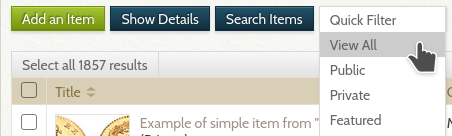
\includegraphics{../_static/images/search-filter.png}

  \begin{enumerate}
  \def\labelenumii{\alph{enumii}.}
  \tightlist
  \item
    \emph{View all} (por defecto): ver todos los ítems.
  \item
    \emph{Public}: ver ítems públicos.
  \item
    \emph{Private}: ver ítems privados.
  \item
    \emph{Featured}: ver ítems destacados.
  \end{enumerate}
\end{enumerate}

\hypertarget{editareliminar-varios-uxedtems-a-la-vez}{%
\paragraph{Editar/Eliminar varios ítems a la
vez}\label{editareliminar-varios-uxedtems-a-la-vez}}

La aplicación te permite modificar o eliminar varios ítems a la vez
desde el gestor de ítems.

\begin{figure}
\hypertarget{batch-edit-view}{%
\centering
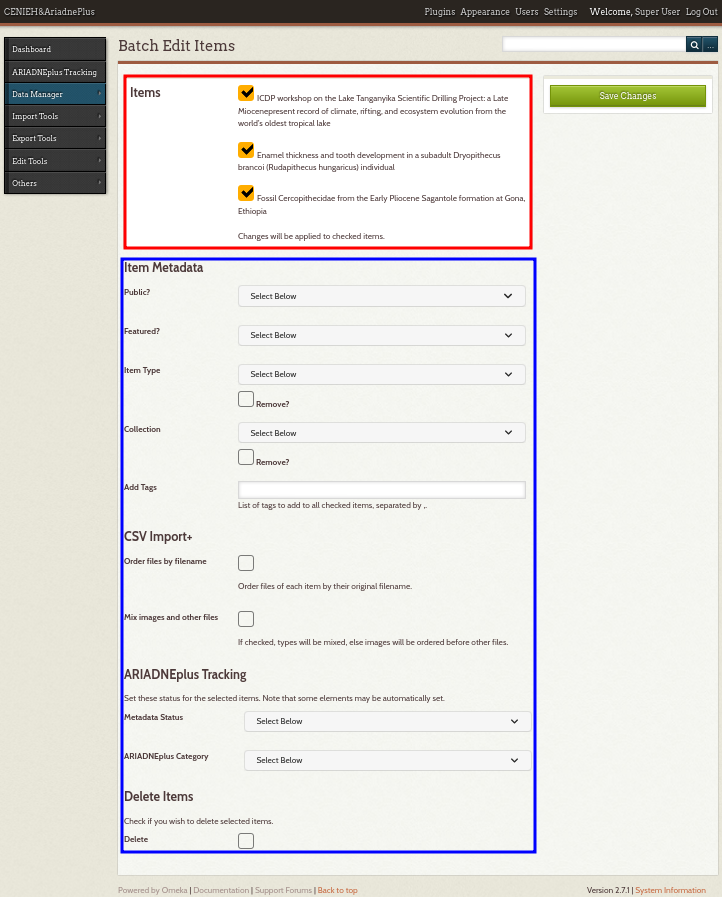
\includegraphics{../_static/images/batch-edit-view.png}
\caption{Vista utilizada para la edición masiva de
ítems}\label{batch-edit-view}
}
\end{figure}

Para editar/eliminar varios ítems a la vez:

\begin{enumerate}
\def\labelenumi{\arabic{enumi}.}
\tightlist
\item
  Desde el gestor de ítems ({/admin/items/}).
\item
  Buscar los ítems que se quieran eliminar/editar (ver
  \protect\hyperlink{buscar-uxedtems}{Buscar ítems}).
\item
  Marcar la casilla situada en la parte izquierda de la tabla de todos
  los ítems que se pretenden editar/eliminar. Si se desean seleccionar
  todos los ítems, hacer clic sobre el botón "\emph{Select all results}"
  situado en la parte superior izquierda de la tabla. Si se desean
  seleccionar todos los ítems de la página actual, marcar la casilla
  alojada en la cabecera de la tabla.
\item
  Hacer clic sobre el botón "\emph{Edit}" situado en la parte superior
  derecha de la tabla.
\item
  Al pulsar el botón "\emph{Edit}", desde la página actual
  ({/admin/items/batch-edit}) podrás:

  \begin{itemize}
  \tightlist
  \item
    cambiar su accesibilidad (públicos / privados)
  \item
    cambiar su estado (descatados o no destacados)
  \item
    cambiar su tipo
  \item
    cambiar o asociar todos los ítems a una colección
  \item
    añadir etiquetas (\emph{tags})
  \item
    ordenar los ítems seleccionados por el nombre de su fichero
    (\emph{file})
  \item
    eliminar todos los ítems
  \end{itemize}
\item
  Comprobar en la lista de ítems que todos los ítems seleccionados son
  correctos. Desmarcar los que no.
\item
  Hacer clic sobre el botón "\emph{Save Changes}".
\end{enumerate}

\hypertarget{visualizar-un-uxedtem-completo}{%
\paragraph{Visualizar un ítem
completo}\label{visualizar-un-uxedtem-completo}}

En la página principal del gestor de ítems ({/admin/items/}) solo se
pueden visualizar los datos más característicos de cada ítem como su
título o tipo. La aplicación te da la posibilidad de visualizar el ítem
al completo, junto a todos sus metadatos, ficheros, \emph{tags}, etc.

\begin{figure}
\hypertarget{show-items-view}{%
\centering
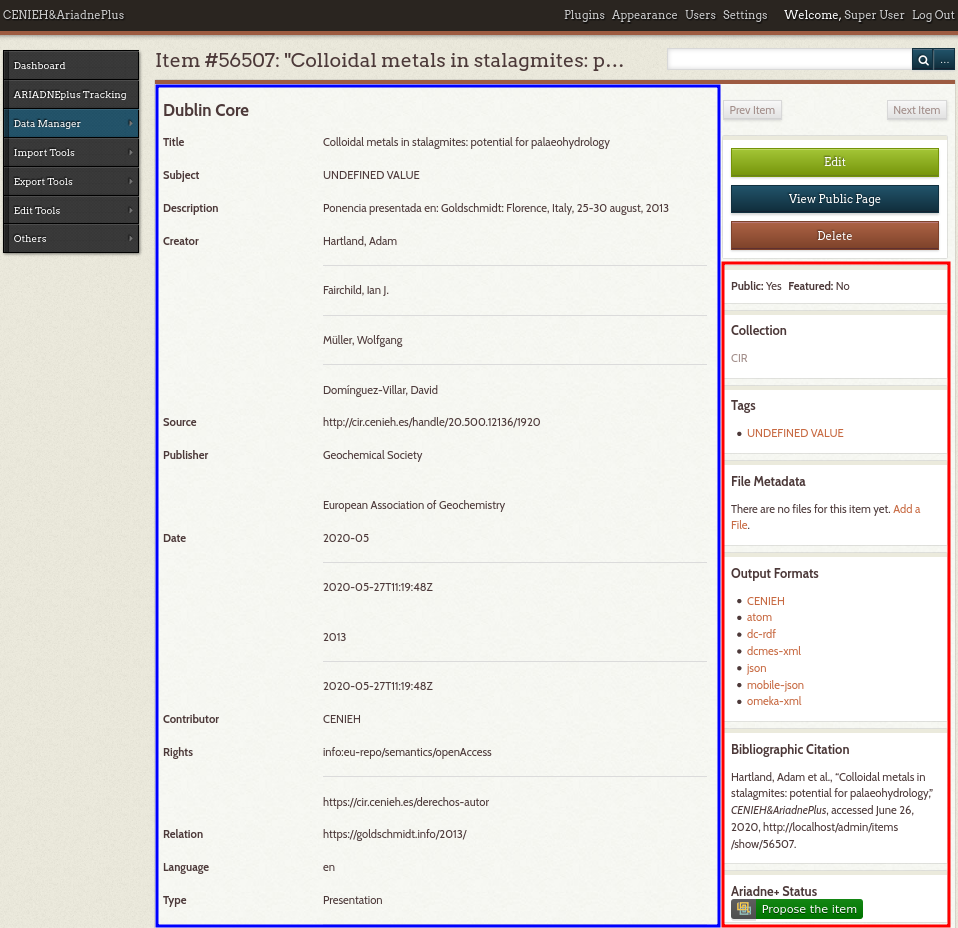
\includegraphics{../_static/images/show-items-view.png}
\caption{Vista utilizada para visualizar ítems}\label{show-items-view}
}
\end{figure}

Para visualizar un ítem:

\begin{enumerate}
\def\labelenumi{\arabic{enumi}.}
\tightlist
\item
  Desde el gestor de ítems ({/admin/items/}).
\item
  Buscar el ítem que se quiera visualizar (ver
  \protect\hyperlink{buscar-uxedtems}{Buscar ítems}).
\item
  Hacer clic sobre el título del ítem, situado en la segunda columna de
  la tabla.
\item
  Visualizar el ítem desde la página actual
  ({/admin/items/show/\textless idItem\textgreater{}}).
\end{enumerate}

\hypertarget{exportar-uxedtems}{%
\paragraph{Exportar ítems}\label{exportar-uxedtems}}

A través de este gestor también se pueden exportar ítems almacenados en
la plataforma. Desde la página principal ({/admin/items/}) se pueden
exportar varios ítems a la vez, sin embargo, desde la página de
visualización ({/admin/items/show/\textless idItem\textgreater{}}) solo
es posible exportar un único ítem. Por este motivo, alguno de los
formatos de exportación disponibles se encontrarán en una sola vista o
en ambas, dependiendo de los requisitos del lenguaje.

\begin{longtable}[]{@{}llll@{}}
\caption{Formato de exportación disponibles para los
Items.}\tabularnewline
\toprule
Formato & Extensión & Disponibilidad & Descripción\tabularnewline
\midrule
\endfirsthead
\toprule
Formato & Extensión & Disponibilidad & Descripción\tabularnewline
\midrule
\endhead
\begin{minipage}[t]{0.22\columnwidth}\raggedright
\emph{atom}\strut
\end{minipage} & \begin{minipage}[t]{0.22\columnwidth}\raggedright
\emph{none}\strut
\end{minipage} & \begin{minipage}[t]{0.22\columnwidth}\raggedright
{/admin/items/}

{/admin/items/show/\textless idItem\textgreater{}}\strut
\end{minipage} & \begin{minipage}[t]{0.22\columnwidth}\raggedright
Esquema de metadatos oficial de \emph{Omeka Classic}\strut
\end{minipage}\tabularnewline
\begin{minipage}[t]{0.22\columnwidth}\raggedright
\emph{dc-rdf}\strut
\end{minipage} & \begin{minipage}[t]{0.22\columnwidth}\raggedright
.rdf\strut
\end{minipage} & \begin{minipage}[t]{0.22\columnwidth}\raggedright
{/admin/items/}

{/admin/items/show/\textless idItem\textgreater{}}\strut
\end{minipage} & \begin{minipage}[t]{0.22\columnwidth}\raggedright
Serialización \href{http://www.jsonml.org/}{JsonML} del esquema
\emph{omeka-xml}.\strut
\end{minipage}\tabularnewline
\begin{minipage}[t]{0.22\columnwidth}\raggedright
\emph{dcmes-xml}\strut
\end{minipage} & \begin{minipage}[t]{0.22\columnwidth}\raggedright
.xml\strut
\end{minipage} & \begin{minipage}[t]{0.22\columnwidth}\raggedright
{/admin/items/}

{/admin/items/show/\textless idItem\textgreater{}}\strut
\end{minipage} & \begin{minipage}[t]{0.22\columnwidth}\raggedright
Instancia \href{https://www.w3.org/TR/rdf-syntax-grammar/}{RDF/XML} del
modelo \href{http://dublincore.org/documents/dcmes-xml/}{Dublin Core}
simple.\strut
\end{minipage}\tabularnewline
\begin{minipage}[t]{0.22\columnwidth}\raggedright
\emph{json}\strut
\end{minipage} & \begin{minipage}[t]{0.22\columnwidth}\raggedright
.json\strut
\end{minipage} & \begin{minipage}[t]{0.22\columnwidth}\raggedright
{/admin/items/}

{/admin/items/show/\textless idItem\textgreater{}}\strut
\end{minipage} & \begin{minipage}[t]{0.22\columnwidth}\raggedright
JSON simplificado utilizado principalmente para solicitudes
\href{https://en.wikipedia.org/wiki/Ajax_(programming)}{Ajax}.\strut
\end{minipage}\tabularnewline
\begin{minipage}[t]{0.22\columnwidth}\raggedright
\emph{mobile-json}\strut
\end{minipage} & \begin{minipage}[t]{0.22\columnwidth}\raggedright
.json\strut
\end{minipage} & \begin{minipage}[t]{0.22\columnwidth}\raggedright
{/admin/items/}

{/admin/items/show/\textless idItem\textgreater{}}\strut
\end{minipage} & \begin{minipage}[t]{0.22\columnwidth}\raggedright
Serialización \href{http://www.jsonml.org/}{JsonML} del modelo
\emph{omeka-xml}.\strut
\end{minipage}\tabularnewline
\begin{minipage}[t]{0.22\columnwidth}\raggedright
\emph{omeka-xml}\strut
\end{minipage} & \begin{minipage}[t]{0.22\columnwidth}\raggedright
.xml\strut
\end{minipage} & \begin{minipage}[t]{0.22\columnwidth}\raggedright
{/admin/items/}

{/admin/items/show/\textless idItem\textgreater{}}\strut
\end{minipage} & \begin{minipage}[t]{0.22\columnwidth}\raggedright
Esquema de metadatos oficial de \emph{Omeka Classic}\strut
\end{minipage}\tabularnewline
\emph{rss2} & .xml & {/admin/items/} & Segunda versión del modelo
\emph{srss}.\tabularnewline
\emph{srss} & .xml & {/admin/items/} & Modelo de metadatos empleado para
la distribución (o sindicación, del inglés \emph{syndication}) de
noticias o información liberada a intervalos de tiempo en sitios web y
weblogs.\tabularnewline
\emph{CENIEH} & .xml &
{/admin/items/show/\textless idItem\textgreater{}} & Esquema de
metadatos empleado para el proceso de integración de datos entre el
CENIEH y ARIADNEplus.\tabularnewline
\emph{CSV} & .csv & {/admin/items/} & Formato abierto sencillo empleado
para representar datos en forma de tabla.\tabularnewline
\bottomrule
\end{longtable}

Para exportar un único ítem:

\begin{enumerate}
\def\labelenumi{\arabic{enumi}.}
\tightlist
\item
  Desde el gestor de ítems ({/admin/items/}).
\item
  Buscar el ítem que se quiera exportar (ver
  \protect\hyperlink{buscar-uxedtems}{Buscar ítems}).
\item
  Hacer clic sobre el título del ítem, situado en la segunda columna de
  la tabla.
\item
  Desde la página de visualización del ítem
  ({/admin/items/show/\textless idItem\textgreater{}}).
\item
  Hacer clic sobre el formato de exportación deseado existente en el
  panel "\emph{Output Formats}" situado en la parte derecha de la
  pantalla (ver \texttt{show-items-view}).
\end{enumerate}

Para exportar todos los ítems de una página:

\begin{enumerate}
\def\labelenumi{\arabic{enumi}.}
\tightlist
\item
  Desde el gestor de ítems ({/admin/items/}).
\item
  Buscar los ítems que se quieran exportar (ver
  \protect\hyperlink{buscar-uxedtems}{Buscar ítems}).
\item
  Hacer clic sobre el formato de exportación deseado de entre todos los
  que se encuentran en parte inferior de la pantalla, justo debajo de la
  tabla de ítems (ver \texttt{items-view}).

  \begin{enumerate}
  \def\labelenumii{\alph{enumii}.}
  \tightlist
  \item
    Para exportar en formato CSV, hay que pulsar el botón situado justo
    debajo de los demás formatos de exportación.
  \end{enumerate}
\end{enumerate}

* \href{https://omeka.org/classic/docs/Content/Items/}{Omeka Classic
User Manual - Items}

\hypertarget{files}{%
\subsubsection{\texorpdfstring{\emph{Files}}{Files}}\label{files}}

Cuando se añaden nuevos ítems a la plataforma, es posible asociar
ficheros (imágenes, documentos, etc.) a los mismos. Por cada uno de
ellos se crea un elemento de tipo \emph{File}, el cual contiene
información detallada del fichero que se ha subido a la plataforma.

Estos elementos no tienen su propia página de gestión ya que son parte
de los ítems, por lo que tiene más sentido que se gestionen desde el
gestor de ítems ({/admin/items/}).

\hypertarget{tipos-de-ficheros-admitidos}{%
\paragraph{Tipos de ficheros
admitidos}\label{tipos-de-ficheros-admitidos}}

La aplicación acepta la gran mayoría de ficheros. Si se tiene algún
error o inconveniente durante la subida de un fichero, consulta en este
mismo manual cómo ajustar los tipos de fichero o extensiones permitidas
en la aplicación.

\hypertarget{tamauxf1o-muxe1ximo-de-ficheros}{%
\paragraph{Tamaño máximo de
ficheros}\label{tamauxf1o-muxe1ximo-de-ficheros}}

Lamentablemente, no se puede configurar el tamaño máximo de los ficheros
desde la aplicación. Para poder modificarlo, es necesario contactar con
el administrador del servidor donde se encuentre alojada la aplicación.

\hypertarget{visualizar-un-fichero}{%
\paragraph{Visualizar un fichero}\label{visualizar-un-fichero}}

A través de la página de visualización de ficheros
({/admin/files/show/\textless idFile\textgreater{}}) es posible obtener
más informacion acerca de un determinado fichero.

\begin{figure}
\hypertarget{show-files-view}{%
\centering
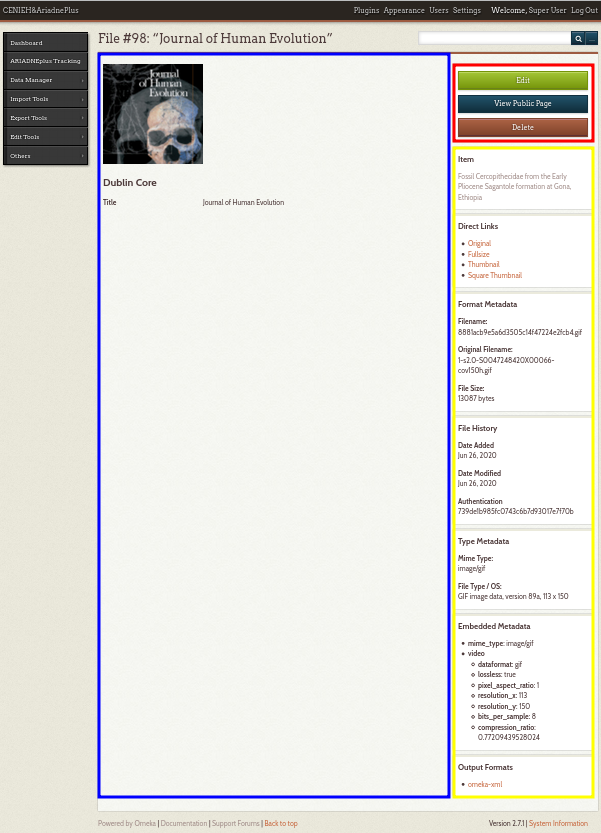
\includegraphics{../_static/images/show-files-view.png}
\caption{Vista utilizada para visualizar
ficheros}\label{show-files-view}
}
\end{figure}

Para visualizar un fichero:

\begin{enumerate}
\def\labelenumi{\arabic{enumi}.}
\tightlist
\item
  Desde el gestor de ítems ({/admin/items/}).
\item
  Buscar el ítem que contenga al archivo involucrado (ver
  \protect\hyperlink{buscar-uxedtems}{Buscar ítems}).
\item
  Hacer clic sobre el título del ítem, situado en la segunda columna de
  la tabla (ver \texttt{items-view}).
\item
  Desde la página actual
  ({/admin/items/show/\textless idItem\textgreater{}}).
\item
  Hacer clic sobre la miniatura del fichero (parte superior, justo
  encima de los metadatos) o bien clicar sobre su nombre (parte derecha,
  panel "\emph{File Metadata}).
\end{enumerate}

\hypertarget{auxf1adir-metadatos-a-un-fichero}{%
\paragraph{Añadir metadatos a un
fichero}\label{auxf1adir-metadatos-a-un-fichero}}

La aplicación permite asociar metadatos del esquema \emph{Dublin Core} a
los ficheros almacenados en la plataforma.

\begin{figure}
\hypertarget{edit-files-view}{%
\centering
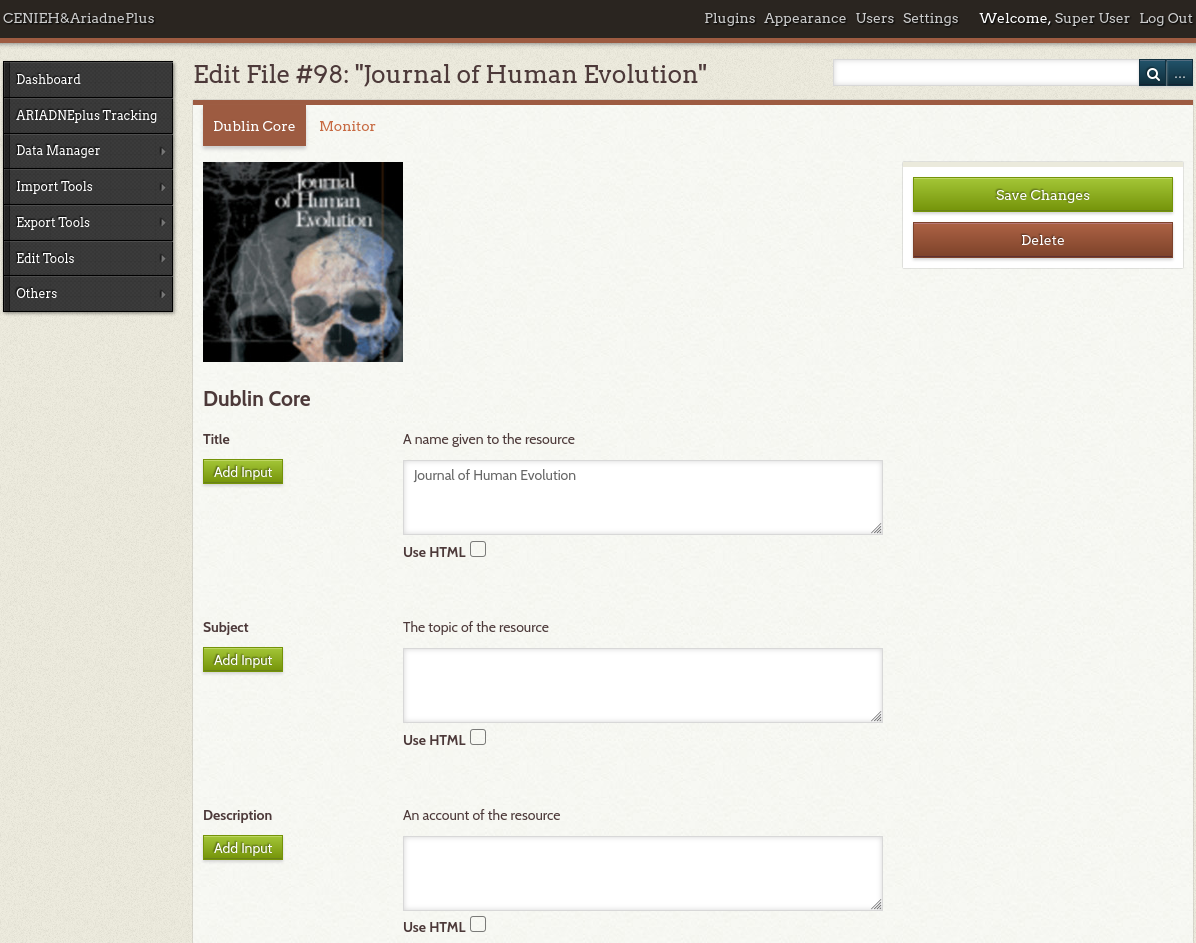
\includegraphics{../_static/images/edit-files-view.png}
\caption{Vista utilizada para editar ficheros}\label{edit-files-view}
}
\end{figure}

{[}Opción 1{]} Para añadir metadatos a un fichero:

\begin{enumerate}
\def\labelenumi{\arabic{enumi}.}
\tightlist
\item
  Desde el gestor de ítems ({/admin/items/}).
\item
  Buscar el ítem que contenga al archivo involucrado (ver
  \protect\hyperlink{buscar-uxedtems}{Buscar ítems}).
\item
  Hacer clic sobre el hipertexto "\emph{Edit}" situado justo debajo del
  título del ítem (ver \texttt{items-view}).
\item
  Desde la página actual
  ({/admin/items/edit/\textless idItem\textgreater{}}), acceder a la
  pestaña "\emph{Files}" (ver \texttt{edit-items-view}).
\item
  Hacer clic sobre el hipertexto "\emph{Edit}" situado en la parte
  derecha del nombre del fichero.
\end{enumerate}

{[}Opción 2{]} Para añadir metadatos a un fichero:

\begin{enumerate}
\def\labelenumi{\arabic{enumi}.}
\tightlist
\item
  Desde el gestor de ítems ({/admin/items/}).
\item
  Buscar el ítem que contenga al archivo involucrado (ver
  \protect\hyperlink{buscar-uxedtems}{Buscar ítems}).
\item
  Hacer clic sobre el título del ítem, situado en la segunda columna de
  la tabla (ver \texttt{items-view}).
\item
  Desde la página actual
  ({/admin/items/show/\textless idItem\textgreater{}}).
\item
  En el panel "\emph{File Metadata}", situado en la parte derecha de la
  pantalla, hacer clic sobre el nombre del fichero al que deseamos
  añadir metadatos (ver \texttt{show-items-view})..
\item
  Desde la página actual
  ({/admin/files/show/\textless idFile\textgreater{}}), hacer clic sobre
  el botón "\emph{Edit}".
\end{enumerate}

* \href{https://omeka.org/classic/docs/Content/Files/}{Omeka Classic
User Manual - Files}

\hypertarget{collections}{%
\subsubsection{\texorpdfstring{\emph{Collections}}{Collections}}\label{collections}}

Las colecciones pueden ser usadas en una gran variedad de contextos en
los que puede tener sentido utilizarlas para tus conjuntos de datos. En
la aplicación, un ítem puede pertenecer a una única colección y, como es
lógico, una colección puede contener múltiple ítems. A través de la
entrada \emph{Collections}, dentro de la sección "\emph{Data Manager}"
del menú principal, se accede al espacio ({/admin/collections}) donde se
gestionan este tipo de elementos.

\begin{figure}
\hypertarget{collections-view}{%
\centering
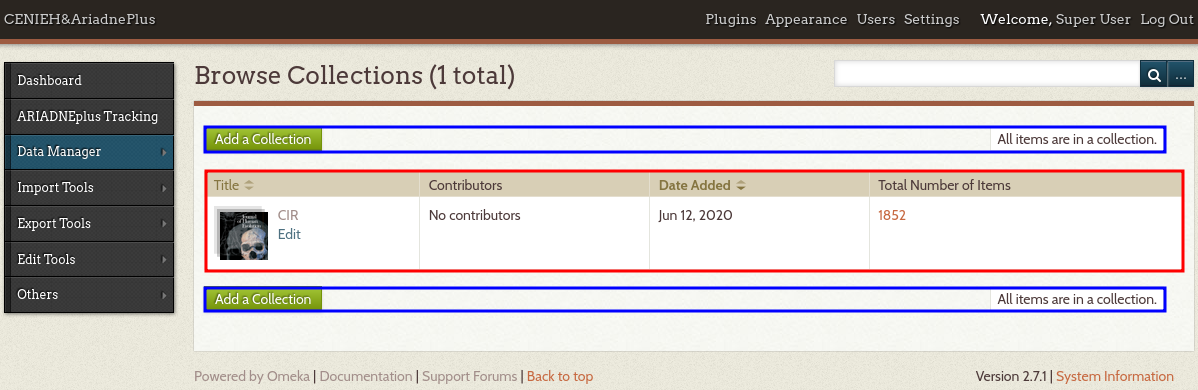
\includegraphics{../_static/images/collections-view.png}
\caption{Vista principal del gestor de
colecciones}\label{collections-view}
}
\end{figure}

\hypertarget{crear-una-colecciuxf3n}{%
\paragraph{Crear una colección}\label{crear-una-colecciuxf3n}}

Antes de poder agrupar ítems en una colección, esta debe ser creada.

\begin{figure}
\hypertarget{add-collections-view}{%
\centering
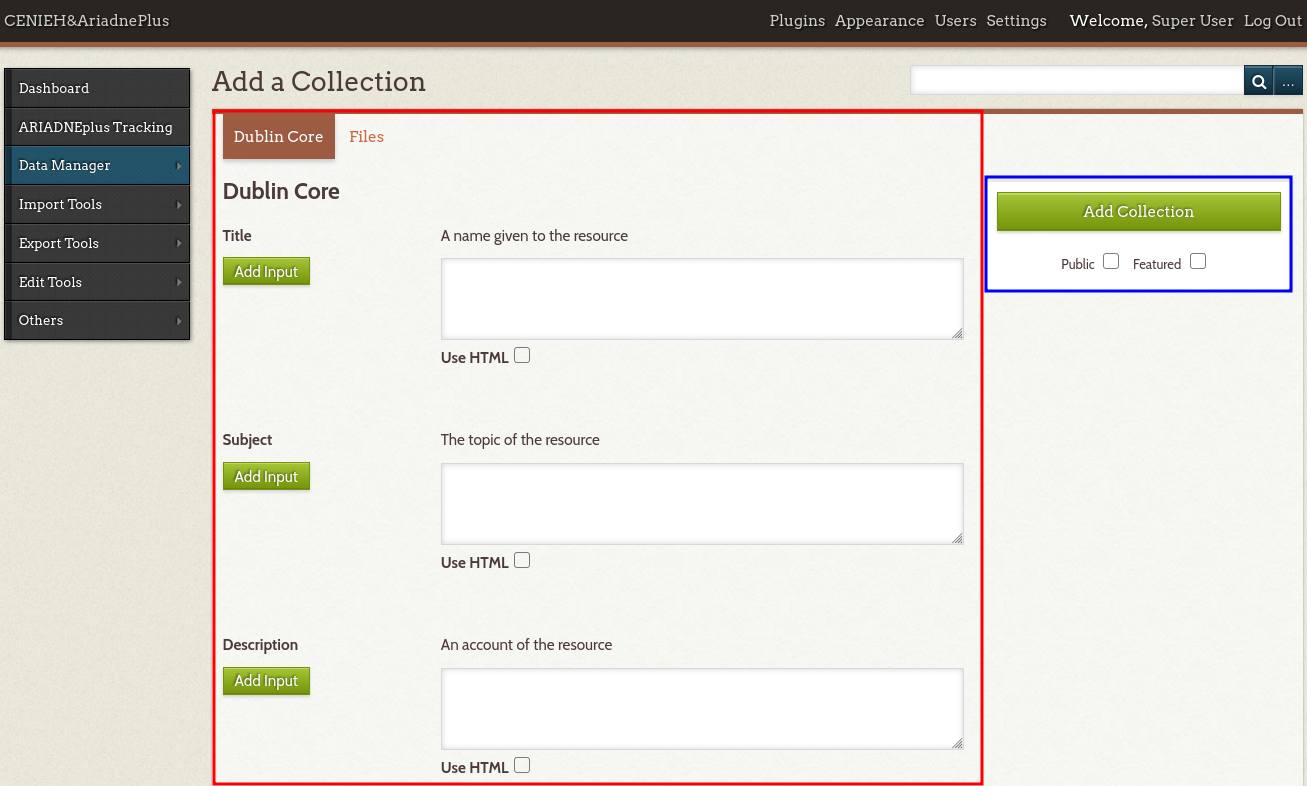
\includegraphics{../_static/images/add-collections-view.png}
\caption{Vista utilizada para crear
colecciones}\label{add-collections-view}
}
\end{figure}

Para crear una colección:

\begin{enumerate}
\def\labelenumi{\arabic{enumi}.}
\tightlist
\item
  Desde el gestor de colecciones ({/admin/collections/}).
\item
  Hacer clic sobre uno de los dos botones "\emph{Add a Collection}".
\item
  En la página actual ({/admin/collections/add}), se puede observar una
  barra de navegación. Desde ella se pueden configurar los elementos de
  la colección:

  \begin{enumerate}
  \def\labelenumii{\alph{enumii}.}
  \tightlist
  \item
    \emph{Dublin Core}: metadatos del esquema \emph{Dublin Core}.
  \item
    \emph{Files}: ficheros asociados.
  \end{enumerate}
\item
  Si se quiere hacer pública la colección, marcar la casilla
  \emph{Public} situada justo debajo del botón "\emph{Add Collection}".
  Además, si se quiere destacar la colección, marcar la casilla
  "\emph{Feature}".
\item
  Hacer clic sobre "\emph{Add Collection}".
\end{enumerate}

\hypertarget{auxf1adir-uxedtems-a-una-colecciuxf3n}{%
\paragraph{Añadir ítems a una
colección}\label{auxf1adir-uxedtems-a-una-colecciuxf3n}}

Las colecciones pueden agrupar un número ilimitado de ítems. Para añadir
ítems a una colección existente se debe señalar a la colección en el
valor especial "\emph{Collection}" de cada ítem. Esta operación no se
puede llevar a cabo desde el gestor de colecciones, debes editar ese
campo desde el gestor de ítems ({/admin/items/}).

Para añadir un solo ítem a una colección:

\begin{figure}
\hypertarget{add-item-collection}{%
\centering
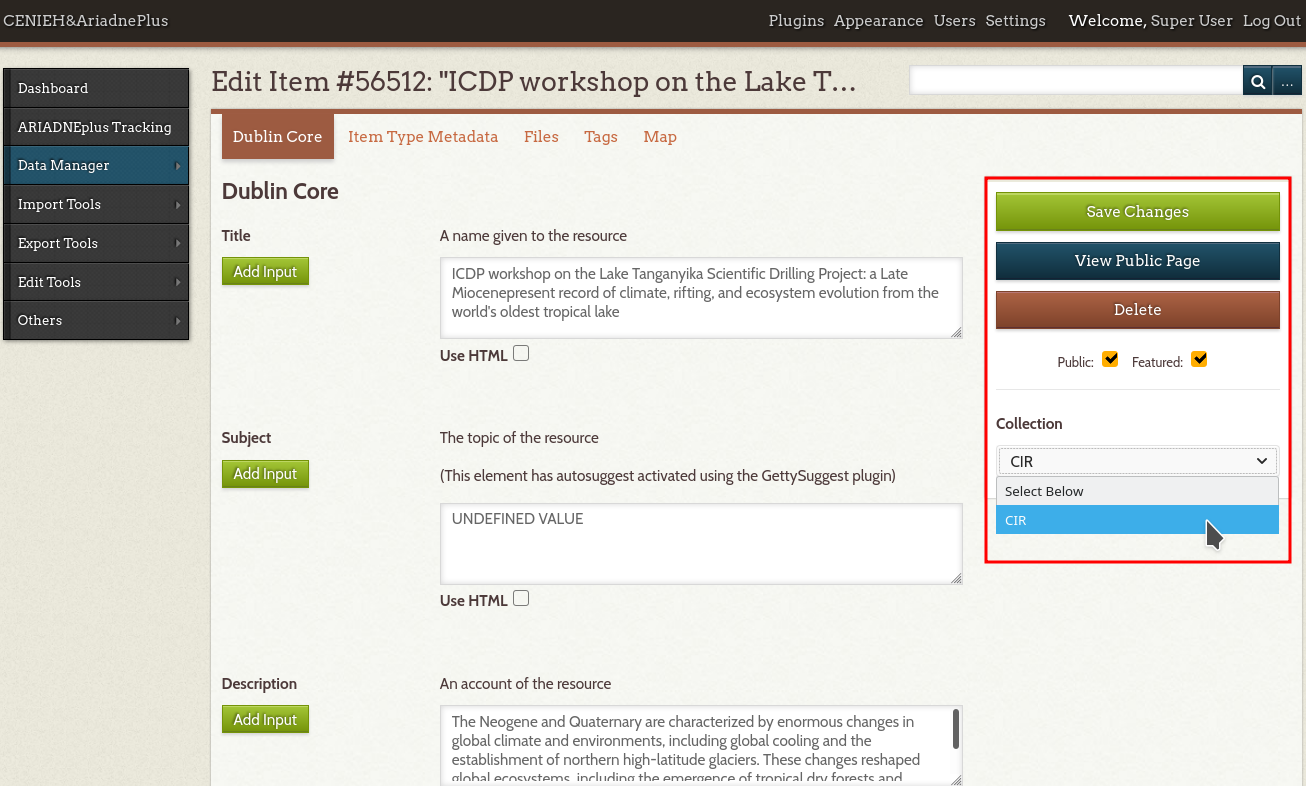
\includegraphics{../_static/images/add-item-collection.png}
\caption{Añadir un ítem a una colección}\label{add-item-collection}
}
\end{figure}

\begin{enumerate}
\def\labelenumi{\arabic{enumi}.}
\tightlist
\item
  Desde el gestor de ítems ({/admin/items/}).
\item
  Localizar la fila en la que se encuentra el ítem y hacer clic sobre el
  hipertexto "\emph{Edit}" situado justo debajo del título del ítem.
\item
  En la página actual
  ({/admin/item/edit/\textless itemid\textgreater{}}), en la parte
  derecha de la pantala, justo debajo del botón "\emph{Add Item}",
  selecciona la colección en el campo "\emph{Collection}".
\item
  Hacer clic sobre el botón "\emph{Save Changes}".
\end{enumerate}

Para añadir varios ítems a una colección:

\begin{figure}
\hypertarget{add-items-collection}{%
\centering
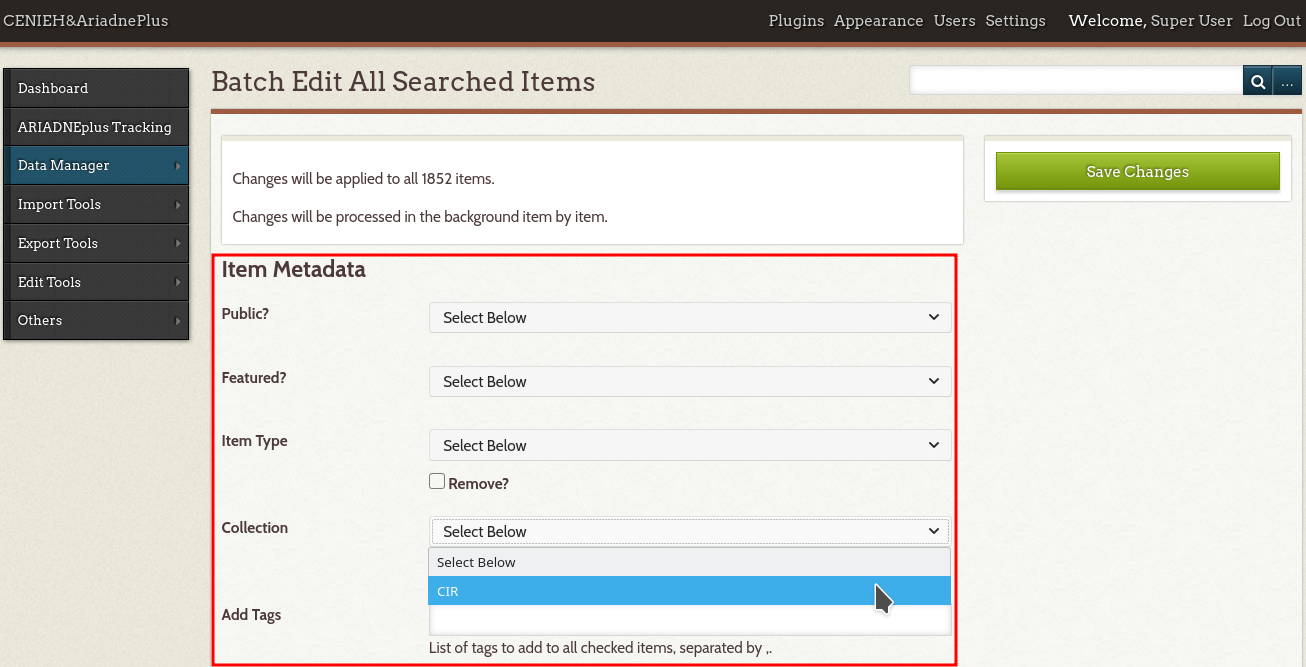
\includegraphics{../_static/images/add-items-collection.png}
\caption{Añadir varios ítems a una
colección}\label{add-items-collection}
}
\end{figure}

\begin{enumerate}
\def\labelenumi{\arabic{enumi}.}
\tightlist
\item
  Desde el gestor de ítems ({/admin/items/}).
\item
  Buscar los ítems que se quieran añadir a la colección.
\item
  Marcar la casilla situada en la parte izquierda de la tabla de todos
  los ítems que se pretenden añadir. Si se desean seleccionar todos los
  ítems, hacer clic sobre el botón "\emph{Select all results}" situado
  en la parte superior izquierda de la tabla. Si se desean seleccionar
  todos los ítems de la página actual, marcar la casilla alojada en la
  cabecera de la tabla.
\item
  Hacer clic sobre el botón "\emph{Edit}" situado en la parte superior
  derecha de la tabla.
\item
  Desde la página actual ({/admin/items/batch-edit}), seleccionar la
  colección en el campo "\emph{Collection}".
\item
  Hacer clic sobre el botón "\emph{Save Changes}".
\end{enumerate}

\hypertarget{editar-una-colecciuxf3n}{%
\paragraph{Editar una colección}\label{editar-una-colecciuxf3n}}

Es posible modificar los datos exclusivos de la colección (no de sus
ítems) una vez haya sido creada.

\begin{figure}
\hypertarget{edit-collections-view}{%
\centering
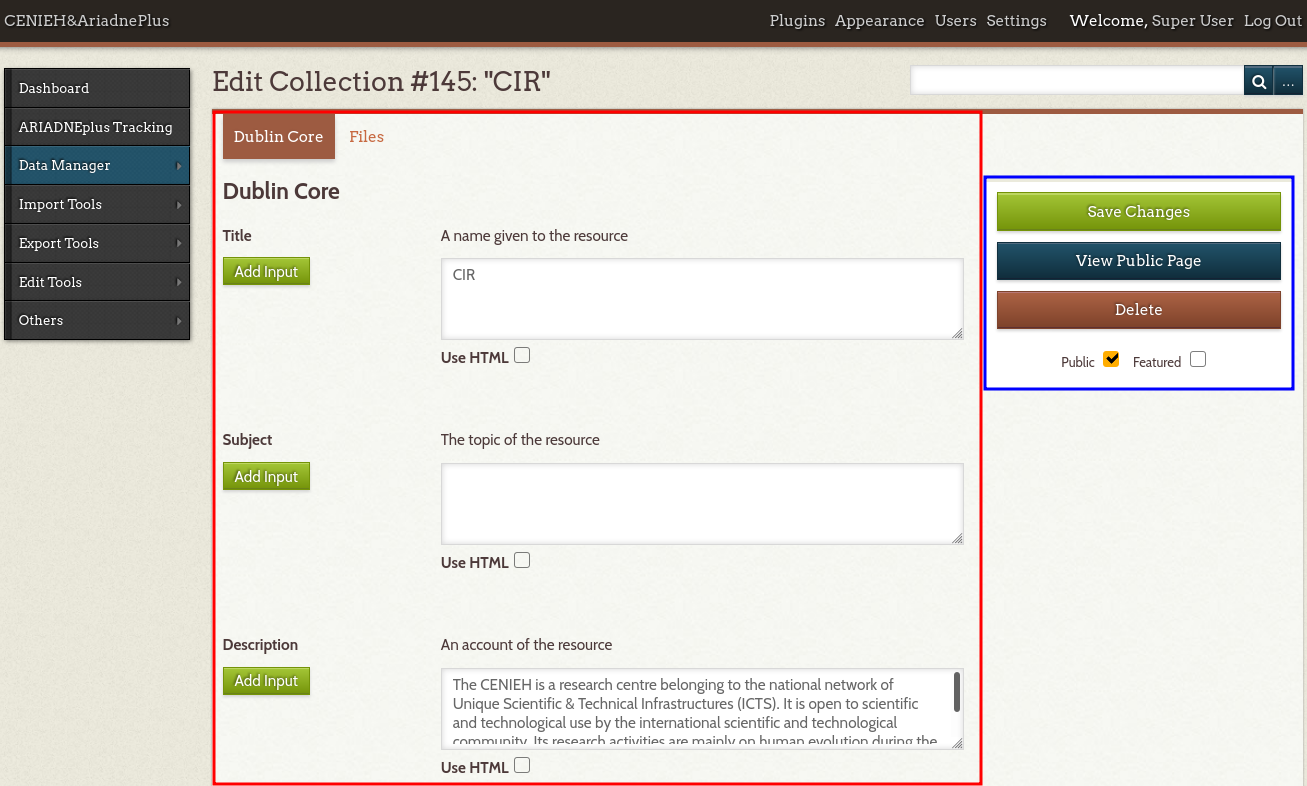
\includegraphics{../_static/images/edit-collections-view.png}
\caption{Vista utilizada para editar
colecciones}\label{edit-collections-view}
}
\end{figure}

Para editar una colección existente:

\begin{enumerate}
\def\labelenumi{\arabic{enumi}.}
\tightlist
\item
  Desde el gestor de colecciones ({/admin/collections/}).
\item
  Hacer clic sobre el hipertexto "\emph{Edit}".
\item
  En la página actual
  ({/admin/collections/edit/\textless collectionId\textgreater{}}),
  realizar las modificaciones oportunas.
\item
  Hacer clic sobre el botón "\emph{Save Changes}".
\end{enumerate}

\hypertarget{eliminar-una-colecciuxf3n.}{%
\paragraph{Eliminar una colección.}\label{eliminar-una-colecciuxf3n.}}

Al eliminar una colección los ítems que estaban asociados a esta no se
eliminan, simplemente se desvinculan. Por tanto, si se pretende eliminar
tanto los ítems como la colección asociada, elimina primero los ítems
asociados a la colección y, posteriormente, elimina la colección.

Para eliminar una colección existente:

\begin{enumerate}
\def\labelenumi{\arabic{enumi}.}
\tightlist
\item
  Desde el gestor de colecciones ({/admin/collections/}).
\item
  Hacer clic sobre el hipertexto "\emph{Edit}".
\item
  En la página actual
  ({/admin/collections/edit/\textless collectionId\textgreater{}}),
  hacer clic sobre el botón "\emph{Delete}".
\item
  Confirmar la eliminación haciendo de nuevo clic sobre el botón
  "\emph{Delete}".
\end{enumerate}

\hypertarget{visualizar-una-colecciuxf3n}{%
\paragraph{Visualizar una colección}\label{visualizar-una-colecciuxf3n}}

Desde la página principal del gestor de colecciones
({/admin/collections/}) solo se muestran algunos datos de cada elemento.
Si queremos conocer más información acerca de una colección, tendremos
que acceder a su página de visualización.

\begin{figure}
\hypertarget{show-collections-view}{%
\centering
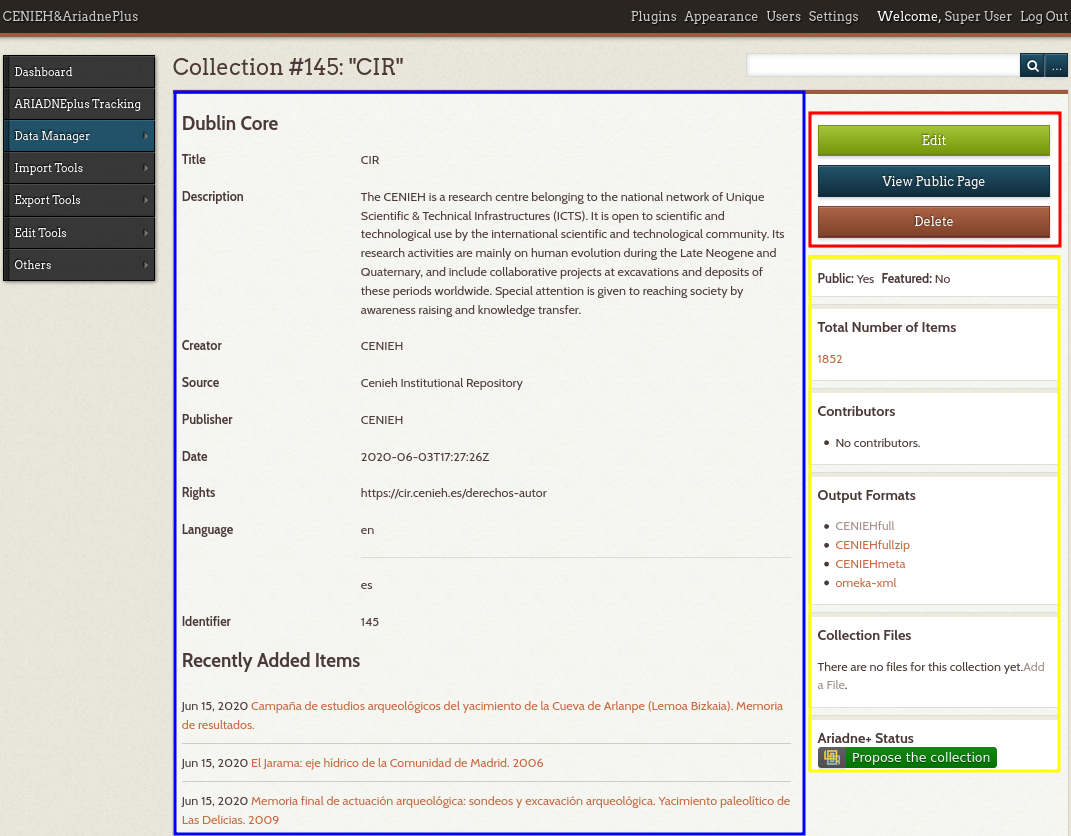
\includegraphics{../_static/images/show-collections-view.png}
\caption{Vista utilizada para visualizar
colecciones}\label{show-collections-view}
}
\end{figure}

Para visualizar una colección:

\begin{enumerate}
\def\labelenumi{\arabic{enumi}.}
\tightlist
\item
  Desde el gestor de colecciones ({/admin/collections/}).
\item
  Buscar la colección que se quiera visualizar.
\item
  Hacer clic sobre el título de la colección, situado en la segunda
  columna de la tabla.
\item
  Visualizar la colección desde la página actual
  ({/admin/collections/show/\textless idItem\textgreater{}}).
\end{enumerate}

* \href{https://omeka.org/classic/docs/Content/Collections/}{Omeka
Classic User Manual - Collections}

\hypertarget{tags}{%
\subsubsection{\texorpdfstring{\emph{Tags}}{Tags}}\label{tags}}

Desde la entrada "\emph{Tags}", dentro de la sección "\emph{Data
Manager}" del menú principal, se accede al gestor de etiquetas o
\emph{tags} ({/admin/tags/}). Las etiquetas son palabras clave o frases
utilizadas para describir los datos almacenados en la plataforma.
Permiten clasificar el contenido de los datos para facilitar su
búsqueda. Estas se pueden asociar a ítems.

\begin{figure}
\hypertarget{tags-view}{%
\centering
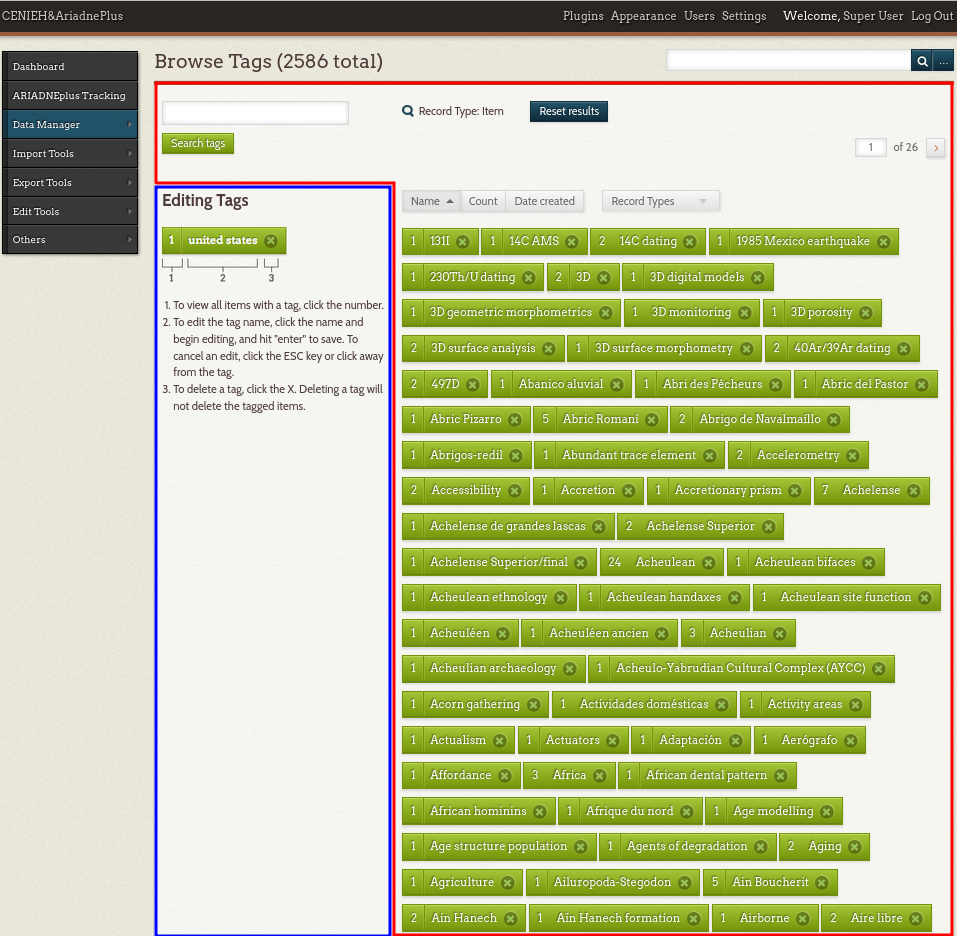
\includegraphics{../_static/images/tags-view.png}
\caption{Vista principal del gestor de etiquetas}\label{tags-view}
}
\end{figure}

Desde el gestor de etiquetas, en la parte derecha se pueden observar
todos los \emph{tags} empleados en cada uno de los ítems existentes en
la plataforma, mientras que en la parte izquierda, al lado del menú
principal, hay un buscador y una explicación de cómo están representados
los \emph{tags}.

\hypertarget{ordenar-tags}{%
\paragraph{\texorpdfstring{Ordenar
\emph{tags}}{Ordenar tags}}\label{ordenar-tags}}

Es posible ordenar las etiquetas en función de su nombre, número de
apariciones, o fecha en la que se creó.

Para ordenar etiquetas:

\begin{enumerate}
\def\labelenumi{\arabic{enumi}.}
\tightlist
\item
  Desde el gestor de etiquetas ({/admin/tags/}).
\item
  Hacer clic sobre alguno de los botones que se encuentran encima del
  conjunto de etiquetas.

  \begin{enumerate}
  \def\labelenumii{\alph{enumii}.}
  \tightlist
  \item
    \emph{Name}: se ordenan alfabéticamente por el nombre de cada
    etiqueta.
  \item
    \emph{Count}: se ordenan en función del número de ítems asociado a
    cada etiqueta.
  \item
    \emph{Date created}: se ordenan por fecha de creación. Por defecto
    más antiguos primero.
  \end{enumerate}
\end{enumerate}

\begin{figure}
\hypertarget{tags-order-buttons}{%
\centering
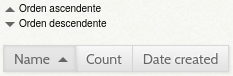
\includegraphics{../_static/images/tags-order-buttons.png}
\caption{Botones para ordenar etiquetas o
tags}\label{tags-order-buttons}
}
\end{figure}

\hypertarget{buscar-tags}{%
\paragraph{\texorpdfstring{Buscar
\emph{tags}}{Buscar tags}}\label{buscar-tags}}

Se pueden buscar etiquetas por su nombre.

\begin{figure}
\hypertarget{tags-search}{%
\centering
\includegraphics{../_static/images/tags-search.png}
\caption{Botones para ordenar etiquetas o tags}\label{tags-search}
}
\end{figure}

Para buscar etiquetas:

\begin{enumerate}
\def\labelenumi{\arabic{enumi}.}
\tightlist
\item
  Desde el gestor de etiquetas ({/admin/tags/}).
\item
  Escribir el nombre de la etiqueta que se está buscando sobre el cuadro
  de texto situado en la parte izquierda de la pantalla.
\item
  Hacer clic sobre el botón "\emph{Search tags}".
\end{enumerate}

Para volver al estado de búsqueda inicial:

\begin{enumerate}
\def\labelenumi{\arabic{enumi}.}
\tightlist
\item
  Desde el gestor de etiquetas ({/admin/tags/}).
\item
  Hacer clic sobre el botón "\emph{Reset results}".
\end{enumerate}

\hypertarget{editar-tags}{%
\paragraph{\texorpdfstring{Editar
\emph{tags}}{Editar tags}}\label{editar-tags}}

Una vez creada una etiqueta, se puede modificar el nombre de esta. Este
cambió se aplicará en todos los ítems que contengan a dicha etiqueta.

\begin{figure}
\hypertarget{tags-edit}{%
\centering
\includegraphics{../_static/images/tags-edit.png}
\caption{Botones para ordenar etiquetas o tags}\label{tags-edit}
}
\end{figure}

Para editar una etiqueta:

\begin{enumerate}
\def\labelenumi{\arabic{enumi}.}
\tightlist
\item
  Desde el gestor de etiquetas ({/admin/tags/}).
\item
  Buscar la etiqueta que se desea editar dentro del conjunto de
  etiquetas situado en la parte derecha de la pantalla.
\item
  Hacer clic sobre el nombre de la etiqueta.
\item
  Introducir el nuevo valor en el campo de texto emergente.
\item
  Pulsar la tecla '\emph{Enter}' o clicar sobre cualquier punto externo.
\end{enumerate}

\hypertarget{eliminar-tags}{%
\paragraph{\texorpdfstring{Eliminar
\emph{tags}}{Eliminar tags}}\label{eliminar-tags}}

Es posible eliminar una o varias etiquetas a la vez. Es importante
recalcar que, cuando se elimina una etiqueta, los ítems que están
asociados no no se eliminan, simplemente se desvinculan de esta.

Para eliminar una sola etiqueta:

\begin{enumerate}
\def\labelenumi{\arabic{enumi}.}
\tightlist
\item
  Desde el gestor de etiquetas ({/admin/tags/}).
\item
  Buscar la etiqueta que se desea eliminar dentro del conjunto de
  etiquetas situado en la parte derecha de la pantalla.
\item
  Hacer clic sobre botón "\emph{x}" situado en la parte derecha de la
  etiqueta.
\item
  Confirmar la eliminación haciendo clic sobre el botón "\emph{Delete}".
\end{enumerate}

Para eliminar varias etiquetas a la vez:

\begin{enumerate}
\def\labelenumi{\arabic{enumi}.}
\tightlist
\item
  Desde el gestor de etiquetas ({/admin/tags/}).
\item
  Buscar las etiquetas que se desean eliminar haciendo uso del buscador.
  Si se desean eliminar todas las etiquetas, ignorar este paso.
\item
  Hacer clic sobre botón rojo "\emph{Delete results}" en caso de haber
  hecho una búsqueda, sino, hacer clic sobre el botón "\emph{Delete
  all}".
\item
  Confirmar la eliminación haciendo clic sobre el botón "\emph{Yes}".
\end{enumerate}

\hypertarget{ver-uxedtems-asociados-a-una-etiqueta}{%
\paragraph{Ver ítems asociados a una
etiqueta}\label{ver-uxedtems-asociados-a-una-etiqueta}}

Se pueden obtener todos los ítems asociados a una determinada etiqueta.

Para ello:

\begin{enumerate}
\def\labelenumi{\arabic{enumi}.}
\tightlist
\item
  Desde el gestor de etiquetas ({/admin/tags/}).
\item
  Buscar la etiqueta que se desea eliminar dentro del conjunto de
  etiquetas situado en la parte derecha de la pantalla.
\item
  Hacer clic sobre el contador situado en la parte izquierda de la
  etiqueta.
\end{enumerate}

* \href{https://omeka.org/classic/docs/Content/Tags/}{Omeka Classic User
Manual - Tags}

\hypertarget{item-types}{%
\subsubsection{\texorpdfstring{\emph{Item
Types}}{Item Types}}\label{item-types}}

Cada ítem puede pertenecer a un determinado tipo, el cual aporta
elementos extra al ítem. Por ejemplo, si un ítem hace referencia a una
persona, puede resultar interesante indicar su fecha de nacimiento,
fecha de muerte, ocupación, etc. Como el esquema de metadatos principal
(\emph{Dublin Core}) no contiene elementos que cubran esta información,
atribuyendo un tipo al ítem se pueden incluir nuevos elementos que
satisfazcan esa necesidad.

\begin{figure}
\hypertarget{item-type-view}{%
\centering
\includegraphics{../_static/images/item-type-view.png}
\caption{Vista principal del gestor de tipos de
ítem.}\label{item-type-view}
}
\end{figure}

A través de la entrada "\emph{Item Types}", dentro de la sección
"\emph{Data Manager}" del menú principal de administración, se puede
acceder al gestor de tipos de ítem ({/admin/item-types}).

\hypertarget{tipos-de-uxedtem-predefinidos}{%
\paragraph{Tipos de ítem
predefinidos}\label{tipos-de-uxedtem-predefinidos}}

Cuando se accede al gestor de tipos de ítem ({/admin/item-types}) por
primera vez se observan un conjunto de tipos de ítems ya definidos.

\begin{longtable}[]{@{}lll@{}}
\caption{Tipos de ítem predefinidos.}\tabularnewline
\toprule
Tipo de ítem & Descripción & Ejemplos\tabularnewline
\midrule
\endfirsthead
\toprule
Tipo de ítem & Descripción & Ejemplos\tabularnewline
\midrule
\endhead
\textbf{Text} & Recurso cuyo principal contenido es texto & Poemas,
libros, cartas, artículos, etc.\tabularnewline
\textbf{Moving Image} & Conjunto de imágenes que puestas en sucesión
imparten una sensación de movimiento & Animaciones, videos, películas,
etc.\tabularnewline
\textbf{Oral History} & Recurso que contiene datos históricos obtenidos
a partir de conferencias, charlas o reuniones. & Charlas, conferencias,
entrevistas, etc.\tabularnewline
\textbf{Sound} & Recurso cuyo principal cometido es ser escuchado. &
Audios de cualquier tipo\tabularnewline
\textbf{Still Image} & Representación visual estática. & Pinturas,
dibujos, planos, mapas, etc.\tabularnewline
\textbf{Website} & Recurso almacenado en una o varias páginas web. &
Página web\tabularnewline
\textbf{Event} & Ocurrencia no persistente basada en el tiempo. &
Conferencia, \emph{Workshop}, Exhibición, etc.\tabularnewline
\textbf{Email} & Recurso cuyo contenido es el propio de un mensaje de
correo electrónido (asunto, cuerpo, origen, destino, etc.) & Mensaje de
correo electrónico\tabularnewline
\textbf{Leson Plan} & Recurso cuyo contenido ofrece una descripción
detallada de un curso de formación. & Curso de formación\tabularnewline
\textbf{Hyperlink} & Recurso existente en Internet. & Enlace,
Referencia, etc.\tabularnewline
\textbf{Person} & Un individuo. & Persona.\tabularnewline
\textbf{Interactive Resource} & Recurso que requiere la interacción del
usuario para ser entenido, ejecutado o experimentado & Formularios,
Aplicaciones, Entornos virtuales, etc.\tabularnewline
\textbf{Dataset} & Datos codificados en una determinada estructura. &
Metadatos.\tabularnewline
\textbf{Physical Object} & Objeto o sustancia inanimada. & Cualquier
objeto físico (e.g una piedra).\tabularnewline
\textbf{Service} & Sistema que provee una o más funciones. & Servicio de
repostería, autentificación, bancario, etc.\tabularnewline
\textbf{Software} & Programa de ordenador. & Archuvos .java, .exe,
etc.\tabularnewline
\textbf{Curatescape Story} & Historia narrativa que puede ser
representada de forma especial por el tema \emph{Curatescape}. & Rutas,
viajes, etc.\tabularnewline
\bottomrule
\end{longtable}

\hypertarget{editar-un-tipo-de-uxedtem}{%
\paragraph{Editar un tipo de ítem}\label{editar-un-tipo-de-uxedtem}}

Se pueden modificar tipos de ítem existentes para modificar sus
elementos (metadatos).

\begin{figure}
\hypertarget{edit-item-type}{%
\centering
\includegraphics{../_static/images/edit-item-type.png}
\caption{Vista desde donde se edita un tipo de
ítem}\label{edit-item-type}
}
\end{figure}

Para modificar un tipo de ítem existente:

\begin{enumerate}
\def\labelenumi{\arabic{enumi}.}
\tightlist
\item
  Desde el gestor de tipos de ítem ({/admin/item-types}).
\item
  Localizar el tipo de ítem que se desea editar en la tabla donde se
  encuentran todos los tipos (ver \texttt{item-type-view}).
\item
  Hacer clic sobre el hipertexto "\emph{Edit}", situado justo debajo del
  nombre del tipo.
\item
  En la página actual
  ({/admin/item-types/edit/\textless idItemType\textgreater{}}),
  realizar las modificaciones oportunas (ver
  \protect\hyperlink{crear-un-tipo-de-uxedtem}{Crear un tipo de ítem}).
\item
  Hacer clic sobre el botón "\emph{Save changes}" situado en la parte
  superior derecha de la pantalla.
\end{enumerate}

\hypertarget{crear-un-tipo-de-uxedtem}{%
\paragraph{Crear un tipo de ítem}\label{crear-un-tipo-de-uxedtem}}

En caso de que ninguno de los tipos de ítem predefinidos (ver
\texttt{itemtypes}) cubra nuestras necesidades, se puede crear un nuevo
tipo de ítem.

\begin{figure}
\hypertarget{add-item-type}{%
\centering
\includegraphics{../_static/images/add-item-type.png}
\caption{Vista desde donde se añade un tipo de
ítem}\label{add-item-type}
}
\end{figure}

Para crear un tipo de ítem nuevo:

\begin{enumerate}
\def\labelenumi{\arabic{enumi}.}
\item
  Desde el gestor de tipos de ítem ({/admin/item-types}).
\item
  Hacer clic sobre el botón "\emph{Add an Item Type}", situado en la
  parte superior/inferior de la pantalla (ver \texttt{item-type-view}).
\item
  En la página actual ({/admin/item-types/add}):

  3.1. Establecer un nombre

  \includegraphics{../_static/images/name-item-type.png}

  3.2. Establecer una descripción

  \includegraphics{../_static/images/desc-item-type.png}

  3.3. Añadir un elemento existente.

  \begin{quote}
  3.3.1. Seleccionar "\emph{Existing}".

  3.3.2. Hacer clic sobre el botón "\emph{Add element}".

  \includegraphics{../_static/images/exi-item-type-1.png}

  3.3.3. En el bloque del elemento emergente, seleccionar el elemento
  existente.

  \includegraphics{../_static/images/exi-item-type-2.png}
  \end{quote}

  3.4. Añadir un elemento nuevo

  \begin{quote}
  \begin{enumerate}
  \def\labelenumii{\arabic{enumii}.}
  \tightlist
  \item
    Seleccionar "\emph{New}".
  \item
    Hacer clic sobre el botón "\emph{Add element}".
  \end{enumerate}

  \includegraphics{../_static/images/new-item-type-1.png}

  \begin{enumerate}
  \def\labelenumii{\arabic{enumii}.}
  \setcounter{enumii}{2}
  \tightlist
  \item
    En el bloque del elemento emergente, establecer el nombre y
    descripción del elemento.
  \end{enumerate}

  \includegraphics{../_static/images/new-item-type-2.png}
  \end{quote}
\item
  Hacer clic sobre el botón "\emph{Add Item Type}" situado en la parte
  superior derecha de la pantalla.
\end{enumerate}

\hypertarget{visualizar-un-tipo-de-uxedtem}{%
\paragraph{Visualizar un tipo de
ítem}\label{visualizar-un-tipo-de-uxedtem}}

Antes de realizar tareas de gestión sobre un determinado tipo de ítem,
se puede comprobar el estado actual del mismo.

\begin{figure}
\hypertarget{show-item-type}{%
\centering
\includegraphics{../_static/images/show-item-type.png}
\caption{Vista desde donde se visualiza un tipo de
ítem}\label{show-item-type}
}
\end{figure}

Para visualizar un tipo de ítem existente.

\begin{enumerate}
\def\labelenumi{\arabic{enumi}.}
\tightlist
\item
  Desde el gestor de tipos de ítem ({/admin/item-types}).
\item
  Localizar el tipo de ítem que se desea eliminar en la tabla donde se
  encuentran todos los tipos (ver \texttt{item-type-view}).
\item
  Hacer clic sobre el nombre del tipo de ítem.
\item
  Visualizar el tipo de ítem en la página actual
  ({/admin/item-types/show/\textless idItemType\textgreater{}}).
\end{enumerate}

\hypertarget{eliminar-un-tipo-de-item}{%
\paragraph{Eliminar un tipo de item}\label{eliminar-un-tipo-de-item}}

Al eliminar un tipo de ítem no se eliminan los elementos (metadatos)
asignados al tipo de ítem. Sin embargo, todos los ítems que tengan
asignado el tipo de ítem eliminado, perderán todos los metadatos
especificados por el tipo de ítem.

{[}Opción 1{]} Para eliminar un tipo de ítem existente:

\begin{enumerate}
\def\labelenumi{\arabic{enumi}.}
\tightlist
\item
  Desde el gestor de tipos de ítem ({/admin/item-types}).
\item
  Localizar el tipo de ítem que se desea eliminar en la tabla donde se
  encuentran todos los tipos (ver \texttt{item-type-view}).
\item
  Hacer clic sobre el hipertexto "\emph{Edit}", situado justo debajo del
  nombre del tipo.
\item
  En la página actual
  ({/admin/item-types/edit/\textless idItemType\textgreater{}}), hacer
  clic sobre el botón rojo "\emph{Delete}" (ver
  \texttt{show-item-type}).
\item
  Confirmar la eliminación volviendo a pulsar sobre el botón
  "\emph{Delete}".
\end{enumerate}

{[}Opción 2{]} Para eliminar un tipo de ítem existente:

\begin{enumerate}
\def\labelenumi{\arabic{enumi}.}
\tightlist
\item
  Desde el gestor de tipos de ítem ({/admin/item-types}).
\item
  Localizar el tipo de ítem que se desea eliminar en la tabla donde se
  encuentran todos los tipos (ver \texttt{item-type-view}).
\item
  Hacer clic sobre el nombre del tipo de ítem.
\item
  En la página actual
  ({/admin/item-types/show/\textless idItemType\textgreater{}}), hacer
  clic sobre el botón rojo "\emph{Delete}".
\item
  Confirmar la eliminación volviendo a pulsar sobre el botón
  "\emph{Delete}".
\end{enumerate}

\href{https://omeka.org/classic/docs/Content/Item_Types/}{Omeka Classic
User Manual - Item Types}

\hypertarget{complementos-plugins}{%
\subsection{\texorpdfstring{Complementos
(\emph{plugins})}{Complementos (plugins)}}\label{complementos-plugins}}

\hypertarget{csv-import}{%
\subsubsection{\texorpdfstring{\emph{CSV
Import+}}{CSV Import+}}\label{csv-import}}

Este complemento nos ofrece una herramienta que nos permite importar
conjuntos de datos que están dispuestos en formato CSV. Se puede acceder
a esta herramienta ({/admin/csv-import-plus/}) desde el menú principal
de navegación a través de la entrada "\emph{CSV Import+}", dentro de la
sección "\emph{Import Tools}".

\begin{figure}
\hypertarget{csv-import-plus-1}{%
\centering
\includegraphics{../_static/images/csv-import-plus-1.png}
\caption{Vista principal de la herramienta CSV
Import+}\label{csv-import-plus-1}
}
\end{figure}

Cuando se accede a esta herramienta, se nos muestra el primer paso a
realizar para llevar a cabo la importación (ver
\texttt{csv-import-plus-1}). Este es un formulario donde el usuario debe
configurar los aspectos de la importación.

\begin{figure}
\hypertarget{csv-import-plus-2}{%
\centering
\includegraphics{../_static/images/csv-import-plus-2.png}
\caption{Vista correspondiente al paso 2 del proceso de importación de
la herramienta CSV Import+}\label{csv-import-plus-2}
}
\end{figure}

Además, existe un segundo paso opcional, donde se lleva a cabo el mapeo
de datos de forma manual (ver \texttt{csv-import-plus-2}).

\begin{figure}
\hypertarget{csv-import-plus-status}{%
\centering
\includegraphics{../_static/images/csv-import-plus-status.png}
\caption{Vista desde donde se visualizan los registros de la herramienta
CSV Import+}\label{csv-import-plus-status}
}
\end{figure}

Tras finalizar el recorrido de importación, es posible visualizar el
registro de cada importación desde la misma herramienta
({/admin/csv-import-plus/}), dentro de la pestaña "\emph{Status}".

\hypertarget{importar-datos-csv}{%
\paragraph{Importar datos CSV}\label{importar-datos-csv}}

Antes de iniciar este proceso, es muy importante que el usuario que lo
lleve a cabo conozca los datos que está importando para configurar
adecuadamente el proceso de importación.

Para importar datos CSV:

\begin{enumerate}
\def\labelenumi{\arabic{enumi}.}
\tightlist
\item
  Desde el complemento \emph{CSV Import+} ({/admin/csv-import-plus/}).
\item
  En la pestaña \emph{Import} (ver \texttt{csv-import-plus-1}), rellenar
  el formulario correspondiente al paso 1 (\emph{Step 1: Select file and
  item settings}). \textbf{Es muy recomendable} dejar los valores por
  defecto (ver \texttt{formImport}).

  \begin{enumerate}
  \def\labelenumii{\alph{enumii}.}
  \tightlist
  \item
    Hacer clic sobre el botón "\emph{Next}".
  \end{enumerate}
\item
  Al seleccionar la opción \emph{Perhaps, so the mapping should be done
  manually} para el campo \emph{Contains extra data}, se debe completar
  un segundo paso (ver \texttt{csv-import-plus-2}) :

  \begin{enumerate}
  \def\labelenumii{\alph{enumii}.}
  \tightlist
  \item
    Establecer las relaciones entre los elementos de origen (e.g
    \emph{Localización}) y los elementos de destino (e.g. \emph{Dublin
    Core:Spatial Coverage}) haciendo uso de la columna \emph{Map To
    Element}.
  \item
    Si alguno de los elementos tiene contenido HTML, indícalo en la
    columna \emph{Use HTML?}.
  \item
    Si alguno de los elementos representa un valor especial (ver
    \texttt{specialvalues}), selecciona dicho valor en la columna
    \emph{Special Values}.

    \begin{itemize}
    \tightlist
    \item
      \textbf{Es obligatorio} que el conjunto de datos cuente con un
      único elemento que contega el identificador de cada registro.
      Luego siempre existirá un elemento con el valor especial
      \emph{Identifier}.
    \end{itemize}
  \item
    Si alguno de los elementos no pertenece a ningún elemento
    estandarizado, sino que pertenece a otro elemento de otro tipo de
    objeto, se debe indicar en la casilla \emph{Extra Data?}.
  \item
    Hacer clic sobre el botón \emph{Import CSV file}.
  \end{enumerate}
\item
  Puedes visualizar el progreso de la importación desde la pestaña
  \emph{Status} (ver \texttt{csv-import-plus-status}).
\end{enumerate}

\hypertarget{tablas-de-configuraciuxf3n}{%
\paragraph{Tablas de configuración}\label{tablas-de-configuraciuxf3n}}

\begin{longtable}[]{@{}llll@{}}
\caption{Formulario de configuración de la herramienta de importación
CSV Import+}\tabularnewline
\toprule
Sección & Campo & Valor & Valor por defecto\tabularnewline
\midrule
\endfirsthead
\toprule
Sección & Campo & Valor & Valor por defecto\tabularnewline
\midrule
\endhead
\textbf{Upload}: adjuntar el fichero CSV a importar & \textbf{Upload CSV
file}: fichero CSV que se pretende importar. & &\tabularnewline
\begin{minipage}[t]{0.22\columnwidth}\raggedright
\textbf{CSV Format}: configurar el formato CSV del fichero adjuntado

\begin{quote}
\begin{itemize}
\tightlist
\item
\item
\item
\item
\end{itemize}
\end{quote}\strut
\end{minipage} & \begin{minipage}[t]{0.22\columnwidth}\raggedright
\begin{quote}
\textbf{Column Delimiter}: caracter utilizado para separar las columnas.
\end{quote}

\begin{description}
\item[-\/-\/-\/-\/-\/-\/-\/-\/-\/-\/-\/-\/-\/-\/-\/-\/-\/-\/-\/-\/-\/-\/-\/-\/-\/-\/-\/-\/-\/-\/-\/-\/-\/-\/-\/-\/-\/-\/-\/-\/-\/-\/-\/-\/-\/-\/-\/-\/-\/-\/-\/-\/-\/-\/-\/-\/-\/-\/-\/-\/-\/-\/-\/-\/-\/-\/-\/-\/-\/-\/-\/-\/-\/-\/-\/-\/-\/-\/-\/-\/-\/-\/-\/-\/-\/-\/-\/-\/-\/-\/-\/-\/-\/-\/-\/-\/-\/-\/-\/-\/-\/-\/-\/-\/-\/-\/-\/-\/-\/-\/-\/-\/-\/-\/-\/-\/-\/-\/-\/-\/-\/-\/-\/-\/-\/-\/-\/-\/-\/-\/-\/-\/-\/-\/-\/-\/-\/-\/-\/-\/-\/-\/-\/-\/-\/-\/-\/-\/-\/-\/-\/-\/-\/-\/-\/-\/-\/-\/-\/-\/-\/-\/-\/-\/-\/-\/-\/-\/-\/-\/-\/-\/-\/-+]
\textbf{Enclosure}: caracter utilizado para delimitar las columnas.
\item[-\/-\/-\/-\/-\/-\/-\/-\/-\/-\/-\/-\/-\/-\/-\/-\/-\/-\/-\/-\/-\/-\/-\/-\/-\/-\/-\/-\/-\/-\/-\/-\/-\/-\/-\/-\/-\/-\/-\/-\/-\/-\/-\/-\/-\/-\/-\/-\/-\/-\/-\/-\/-\/-\/-\/-\/-\/-\/-\/-\/-\/-\/-\/-\/-\/-\/-\/-\/-\/-\/-\/-\/-\/-\/-\/-\/-\/-\/-\/-\/-\/-\/-\/-\/-\/-\/-\/-\/-\/-\/-\/-\/-\/-\/-\/-\/-\/-\/-\/-\/-\/-\/-\/-\/-\/-\/-\/-\/-\/-\/-\/-\/-\/-\/-\/-\/-\/-\/-\/-\/-\/-\/-\/-\/-\/-\/-\/-\/-\/-\/-\/-\/-\/-\/-\/-\/-\/-\/-\/-\/-\/-\/-\/-\/-\/-\/-\/-\/-\/-\/-\/-\/-\/-\/-\/-\/-\/-\/-\/-\/-\/-\/-\/-\/-\/-\/-\/-\/-\/-\/-\/-\/-\/-+]
\textbf{Element delimiter}: caracter utilizado para separar metadatos
dentro de una misma celda.
\item[-\/-\/-\/-\/-\/-\/-\/-\/-\/-\/-\/-\/-\/-\/-\/-\/-\/-\/-\/-\/-\/-\/-\/-\/-\/-\/-\/-\/-\/-\/-\/-\/-\/-\/-\/-\/-\/-\/-\/-\/-\/-\/-\/-\/-\/-\/-\/-\/-\/-\/-\/-\/-\/-\/-\/-\/-\/-\/-\/-\/-\/-\/-\/-\/-\/-\/-\/-\/-\/-\/-\/-\/-\/-\/-\/-\/-\/-\/-\/-\/-\/-\/-\/-\/-\/-\/-\/-\/-\/-\/-\/-\/-\/-\/-\/-\/-\/-\/-\/-\/-\/-\/-\/-\/-\/-\/-\/-\/-\/-\/-\/-\/-\/-\/-\/-\/-\/-\/-\/-\/-\/-\/-\/-\/-\/-\/-\/-\/-\/-\/-\/-\/-\/-\/-\/-\/-\/-\/-\/-\/-\/-\/-\/-\/-\/-\/-\/-\/-\/-\/-\/-\/-\/-\/-\/-\/-\/-\/-\/-\/-\/-\/-\/-\/-\/-\/-\/-\/-\/-\/-\/-\/-\/-+]
\textbf{Tag delimiter}: caracter utilizado para separar \emph{tags}
dentro de una misma celda.

\textbf{Si tus datos no contienen tags, puedes ignorarlo}.
\item[-\/-\/-\/-\/-\/-\/-\/-\/-\/-\/-\/-\/-\/-\/-\/-\/-\/-\/-\/-\/-\/-\/-\/-\/-\/-\/-\/-\/-\/-\/-\/-\/-\/-\/-\/-\/-\/-\/-\/-\/-\/-\/-\/-\/-\/-\/-\/-\/-\/-\/-\/-\/-\/-\/-\/-\/-\/-\/-\/-\/-\/-\/-\/-\/-\/-\/-\/-\/-\/-\/-\/-\/-\/-\/-\/-\/-\/-\/-\/-\/-\/-\/-\/-\/-\/-\/-\/-\/-\/-\/-\/-\/-\/-\/-\/-\/-\/-\/-\/-\/-\/-\/-\/-\/-\/-\/-\/-\/-\/-\/-\/-\/-\/-\/-\/-\/-\/-\/-\/-\/-\/-\/-\/-\/-\/-\/-\/-\/-\/-\/-\/-\/-\/-\/-\/-\/-\/-\/-\/-\/-\/-\/-\/-\/-\/-\/-\/-\/-\/-\/-\/-\/-\/-\/-\/-\/-\/-\/-\/-\/-\/-\/-\/-\/-\/-\/-\/-\/-\/-\/-\/-\/-\/-+]
\textbf{File delimiter}: caracter utilizado para separar rutas de
archivos o \emph{URLs} dentro de una misma celda.

\textbf{Si tus datos no referencian ficheros, puedes ignorarlo.}
\end{description}\strut
\end{minipage} & \begin{minipage}[t]{0.22\columnwidth}\raggedright
\begin{quote}
\begin{itemize}
\tightlist
\item
  \textbf{comma}: ','
\item
  \textbf{Semi-colon}: ';'
\item
  \textbf{Colon}: '.'
\item
  \textbf{pipe}: '\textbar'
\item
  \textbf{tabulation}: ' '
\item
  \textbf{carriage return}: '↵'
\item
  \textbf{space}: ' '
\item
  \textbf{custom}: ?
\end{itemize}
\end{quote}

\begin{description}
\item[-\/-\/-\/-\/-\/-\/-\/-\/-\/-\/-\/-\/-\/-\/-\/-\/-\/-\/-\/-\/-\/-\/-\/-\/-\/-\/-\/-\/-\/-\/-\/-\/-\/-\/-\/-\/-\/-\/-\/-\/-\/-\/-\/-\/-\/-\/-\/-\/-\/-\/-\/-\/-\/-\/-\/-\/-\/-\/-\/-\/-\/-\/-\/-\/-\/-\/-\/-\/-\/-\/-\/-\/-\/-\/-\/-\/-\/-\/-\/-\/-\/-\/-\/-\/-\/-\/-\/-\/-\/-\/-\/-\/-\/-\/-\/-\/-\/-\/-\/-\/-\/-\/-\/-\/-\/-\/-\/-\/-\/-\/-\/-\/-\/-\/-\/-\/-\/-\/-\/-\/-\/-\/-\/-\/-\/-\/-\/-\/-+]
\begin{itemize}
\tightlist
\item
  \textbf{double quote}: '"'
\item
  \textbf{single quote}: '''
\item
  \textbf{custom}: ?
\end{itemize}
\item[-\/-\/-\/-\/-\/-\/-\/-\/-\/-\/-\/-\/-\/-\/-\/-\/-\/-\/-\/-\/-\/-\/-\/-\/-\/-\/-\/-\/-\/-\/-\/-\/-\/-\/-\/-\/-\/-\/-\/-\/-\/-\/-\/-\/-\/-\/-\/-\/-\/-\/-\/-\/-\/-\/-\/-\/-\/-\/-\/-\/-\/-\/-\/-\/-\/-\/-\/-\/-\/-\/-\/-\/-\/-\/-\/-\/-\/-\/-\/-\/-\/-\/-\/-\/-\/-\/-\/-\/-\/-\/-\/-\/-\/-\/-\/-\/-\/-\/-\/-\/-\/-\/-\/-\/-\/-\/-\/-\/-\/-\/-\/-\/-\/-\/-\/-\/-\/-\/-\/-\/-\/-\/-\/-\/-\/-\/-\/-\/-+]
\begin{itemize}
\tightlist
\item
  \textbf{comma}: ','
\item
  \textbf{Semi-colon}: ';' +
\item
  \textbf{Colon}: '.'
\item
  \textbf{pipe}: '\textbar'
\item
  \textbf{tabulation}: ' '
\item
  \textbf{carriage return}: '↵' +
\item
  \textbf{space}: ' '
\item
  \textbf{double space}: ' '
\item
  \textbf{custom}: ?
\end{itemize}
\end{description}\strut
\end{minipage} & \begin{minipage}[t]{0.22\columnwidth}\raggedright
\begin{quote}
\textbf{Coma}
\end{quote}

\begin{description}
\item[-\/-\/-\/-\/-\/-\/-\/-\/-\/-\/-\/-\/-\/-\/-\/-\/-\/-\/-\/-\/-\/-\/-\/-\/-\/-\/-\/-\/-\/-\/-\/-\/-\/-\/-\/-\/-\/-\/-\/-\/-\/-\/-\/-\/-\/-\/-\/-\/-\/-\/-\/-\/-+]
\textbf{double quote}
\item[-\/-\/-\/-\/-\/-\/-\/-\/-\/-\/-\/-\/-\/-\/-\/-\/-\/-\/-\/-\/-\/-\/-\/-\/-\/-\/-\/-\/-\/-\/-\/-\/-\/-\/-\/-\/-\/-\/-\/-\/-\/-\/-\/-\/-\/-\/-\/-\/-\/-\/-\/-\/-+]
\textbf{Semi-colon}
\item[-\/-\/-\/-\/-\/-\/-\/-\/-\/-\/-\/-\/-\/-\/-\/-\/-\/-\/-\/-\/-\/-\/-\/-\/-\/-\/-\/-\/-\/-\/-\/-\/-\/-\/-\/-\/-\/-\/-\/-\/-\/-\/-\/-\/-\/-\/-\/-\/-\/-\/-\/-\/-+]
\textbf{comma}
\item[-\/-\/-\/-\/-\/-\/-\/-\/-\/-\/-\/-\/-\/-\/-\/-\/-\/-\/-\/-\/-\/-\/-\/-\/-\/-\/-\/-\/-\/-\/-\/-\/-\/-\/-\/-\/-\/-\/-\/-\/-\/-\/-\/-\/-\/-\/-\/-\/-\/-\/-\/-\/-+]
\textbf{comma}
\end{description}\strut
\end{minipage}\tabularnewline
\begin{minipage}[t]{0.22\columnwidth}\raggedright
\textbf{Default values}: configurar los valores por defecto para todos
los ítems a importar

\begin{quote}
\begin{itemize}
\tightlist
\item
\item
\item
\item
\end{itemize}
\end{quote}\strut
\end{minipage} & \begin{minipage}[t]{0.22\columnwidth}\raggedright
\begin{quote}
\textbf{Item type}: tipo de ítem que pretendemos importar.
\end{quote}

\begin{description}
\item[-\/-\/-\/-\/-\/-\/-\/-\/-\/-\/-\/-\/-\/-\/-\/-\/-\/-\/-\/-\/-\/-\/-\/-\/-\/-\/-\/-\/-\/-\/-\/-\/-\/-\/-\/-\/-\/-\/-\/-\/-\/-\/-\/-\/-\/-\/-\/-\/-\/-\/-\/-\/-\/-\/-\/-\/-\/-\/-\/-\/-\/-\/-\/-\/-\/-\/-\/-\/-\/-\/-\/-\/-\/-\/-\/-\/-\/-\/-\/-\/-\/-\/-\/-\/-\/-\/-\/-\/-\/-\/-\/-\/-\/-\/-\/-\/-\/-\/-\/-\/-\/-\/-\/-\/-\/-\/-\/-\/-\/-\/-\/-\/-\/-\/-\/-\/-\/-\/-\/-\/-\/-\/-\/-\/-\/-\/-\/-\/-\/-\/-\/-\/-\/-\/-\/-\/-\/-\/-\/-\/-\/-\/-\/-\/-\/-\/-\/-\/-\/-\/-\/-\/-\/-\/-\/-\/-\/-\/-\/-\/-\/-\/-\/-\/-\/-\/-\/-\/-\/-\/-\/-\/-\/-+]
\textbf{Collection}: colección a la que pertenecen los ítems.

\textbf{Si el fichero contiene muchos ítems, conviene agruparlos dentro
de una colección previamente creada.}
\item[-\/-\/-\/-\/-\/-\/-\/-\/-\/-\/-\/-\/-\/-\/-\/-\/-\/-\/-\/-\/-\/-\/-\/-\/-\/-\/-\/-\/-\/-\/-\/-\/-\/-\/-\/-\/-\/-\/-\/-\/-\/-\/-\/-\/-\/-\/-\/-\/-\/-\/-\/-\/-\/-\/-\/-\/-\/-\/-\/-\/-\/-\/-\/-\/-\/-\/-\/-\/-\/-\/-\/-\/-\/-\/-\/-\/-\/-\/-\/-\/-\/-\/-\/-\/-\/-\/-\/-\/-\/-\/-\/-\/-\/-\/-\/-\/-\/-\/-\/-\/-\/-\/-\/-\/-\/-\/-\/-\/-\/-\/-\/-\/-\/-\/-\/-\/-\/-\/-\/-\/-\/-\/-\/-\/-\/-\/-\/-\/-\/-\/-\/-\/-\/-\/-\/-\/-\/-\/-\/-\/-\/-\/-\/-\/-\/-\/-\/-\/-\/-\/-\/-\/-\/-\/-\/-\/-\/-\/-\/-\/-\/-\/-\/-\/-\/-\/-\/-\/-\/-\/-\/-\/-\/-+]
\textbf{Make records public}: activado, se publicarán los ítems tras la
importación
\item[-\/-\/-\/-\/-\/-\/-\/-\/-\/-\/-\/-\/-\/-\/-\/-\/-\/-\/-\/-\/-\/-\/-\/-\/-\/-\/-\/-\/-\/-\/-\/-\/-\/-\/-\/-\/-\/-\/-\/-\/-\/-\/-\/-\/-\/-\/-\/-\/-\/-\/-\/-\/-\/-\/-\/-\/-\/-\/-\/-\/-\/-\/-\/-\/-\/-\/-\/-\/-\/-\/-\/-\/-\/-\/-\/-\/-\/-\/-\/-\/-\/-\/-\/-\/-\/-\/-\/-\/-\/-\/-\/-\/-\/-\/-\/-\/-\/-\/-\/-\/-\/-\/-\/-\/-\/-\/-\/-\/-\/-\/-\/-\/-\/-\/-\/-\/-\/-\/-\/-\/-\/-\/-\/-\/-\/-\/-\/-\/-\/-\/-\/-\/-\/-\/-\/-\/-\/-\/-\/-\/-\/-\/-\/-\/-\/-\/-\/-\/-\/-\/-\/-\/-\/-\/-\/-\/-\/-\/-\/-\/-\/-\/-\/-\/-\/-\/-\/-\/-\/-\/-\/-\/-\/-+]
\textbf{Feature}: activado, se marcarán los ítems importados como
\emph{feature}.
\item[-\/-\/-\/-\/-\/-\/-\/-\/-\/-\/-\/-\/-\/-\/-\/-\/-\/-\/-\/-\/-\/-\/-\/-\/-\/-\/-\/-\/-\/-\/-\/-\/-\/-\/-\/-\/-\/-\/-\/-\/-\/-\/-\/-\/-\/-\/-\/-\/-\/-\/-\/-\/-\/-\/-\/-\/-\/-\/-\/-\/-\/-\/-\/-\/-\/-\/-\/-\/-\/-\/-\/-\/-\/-\/-\/-\/-\/-\/-\/-\/-\/-\/-\/-\/-\/-\/-\/-\/-\/-\/-\/-\/-\/-\/-\/-\/-\/-\/-\/-\/-\/-\/-\/-\/-\/-\/-\/-\/-\/-\/-\/-\/-\/-\/-\/-\/-\/-\/-\/-\/-\/-\/-\/-\/-\/-\/-\/-\/-\/-\/-\/-\/-\/-\/-\/-\/-\/-\/-\/-\/-\/-\/-\/-\/-\/-\/-\/-\/-\/-\/-\/-\/-\/-\/-\/-\/-\/-\/-\/-\/-\/-\/-\/-\/-\/-\/-\/-\/-\/-\/-\/-\/-\/-+]
\textbf{Elements are html}: activado, se considerará que el contenido de
los ítems está en html.
\end{description}\strut
\end{minipage} & \begin{minipage}[t]{0.22\columnwidth}\raggedright
\begin{quote}
\begin{itemize}
\tightlist
\item
  \textbf{No default item type}
\item
  \textbf{Tipo de ítem}
\end{itemize}
\end{quote}

\begin{description}
\item[-\/-\/-\/-\/-\/-\/-\/-\/-\/-\/-\/-\/-\/-\/-\/-\/-\/-\/-\/-\/-\/-\/-\/-\/-\/-\/-\/-\/-\/-\/-\/-\/-\/-\/-\/-\/-\/-\/-\/-\/-\/-\/-\/-\/-\/-\/-\/-\/-\/-\/-\/-\/-\/-\/-\/-\/-\/-\/-\/-\/-\/-\/-\/-\/-\/-\/-\/-\/-\/-\/-\/-\/-\/-\/-\/-\/-\/-\/-\/-\/-\/-\/-\/-\/-\/-\/-\/-\/-\/-\/-\/-\/-\/-\/-\/-\/-\/-\/-\/-\/-\/-\/-\/-\/-\/-\/-\/-\/-\/-\/-\/-\/-\/-\/-\/-\/-\/-\/-\/-\/-\/-\/-\/-\/-\/-\/-\/-\/-+]
\begin{itemize}
\tightlist
\item
  \textbf{No default collection}
\item
  \textbf{Colección}
\end{itemize}
\item[-\/-\/-\/-\/-\/-\/-\/-\/-\/-\/-\/-\/-\/-\/-\/-\/-\/-\/-\/-\/-\/-\/-\/-\/-\/-\/-\/-\/-\/-\/-\/-\/-\/-\/-\/-\/-\/-\/-\/-\/-\/-\/-\/-\/-\/-\/-\/-\/-\/-\/-\/-\/-\/-\/-\/-\/-\/-\/-\/-\/-\/-\/-\/-\/-\/-\/-\/-\/-\/-\/-\/-\/-\/-\/-\/-\/-\/-\/-\/-\/-\/-\/-\/-\/-\/-\/-\/-\/-\/-\/-\/-\/-\/-\/-\/-\/-\/-\/-\/-\/-\/-\/-\/-\/-\/-\/-\/-\/-\/-\/-\/-\/-\/-\/-\/-\/-\/-\/-\/-\/-\/-\/-\/-\/-\/-\/-\/-\/-+]
\begin{itemize}
\tightlist
\item
  \textbf{Activado}
\item
  \textbf{Desactivado}
\end{itemize}
\end{description}\strut
\end{minipage} & \begin{minipage}[t]{0.22\columnwidth}\raggedright
\begin{quote}
\textbf{No default item type}
\end{quote}

\begin{description}
\item[-\/-\/-\/-\/-\/-\/-\/-\/-\/-\/-\/-\/-\/-\/-\/-\/-\/-\/-\/-\/-\/-\/-\/-\/-\/-\/-\/-\/-\/-\/-\/-\/-\/-\/-\/-\/-\/-\/-\/-\/-\/-\/-\/-\/-\/-\/-\/-\/-\/-\/-\/-\/-+]
\textbf{No default collection}
\item[-\/-\/-\/-\/-\/-\/-\/-\/-\/-\/-\/-\/-\/-\/-\/-\/-\/-\/-\/-\/-\/-\/-\/-\/-\/-\/-\/-\/-\/-\/-\/-\/-\/-\/-\/-\/-\/-\/-\/-\/-\/-\/-\/-\/-\/-\/-\/-\/-\/-\/-\/-\/-+]
\textbf{Desactivado}
\end{description}\strut
\end{minipage}\tabularnewline
\begin{minipage}[t]{0.22\columnwidth}\raggedright
\textbf{Process}: configurar el proceso de importación.

\textbf{Las opciones por defecto son válidas para cualquier
importación}\strut
\end{minipage} & \begin{minipage}[t]{0.22\columnwidth}\raggedright
\textbf{Identifier field}: elemento que señala el identificador de cada
ítem.\strut
\end{minipage} & \begin{minipage}[t]{0.22\columnwidth}\raggedright
\begin{itemize}
\tightlist
\item
  \textbf{No default identifier field}: no se especifica ningún campo
  como identificador.
\item
  \textbf{Table identifier}: columna "table id" o "Identifier" de la
  tabla CSV del fichero adjuntado.
\item
  \textbf{Internal id}: identificador interno del registro en la
  aplicación.
\item
  \textbf{Elemento}: elemento de algún esquema de metadatos.
\end{itemize}\strut
\end{minipage} & \begin{minipage}[t]{0.22\columnwidth}\raggedright
\textbf{No default identifier field}\strut
\end{minipage}\tabularnewline
\begin{minipage}[t]{0.22\columnwidth}\raggedright
\strut
\end{minipage} & \begin{minipage}[t]{0.22\columnwidth}\raggedright
\textbf{Action}: acción que se ejecutará en cada ítem.

\textbf{Para que estas acciones se ejecuten, el identificador del dato
importado ha de coincidir con el identificador del ítem existente en la
plataforma.}\strut
\end{minipage} & \begin{minipage}[t]{0.22\columnwidth}\raggedright
\begin{itemize}
\tightlist
\item
  \textbf{No default action}: no se ejecuta ninguna acción.
\item
  \textbf{Update record if exist, else create one}: se actualiza el
  registro si existe, sino se crea.
\item
  \textbf{Create a new record}: se crea un nuevo registro.
\item
  \textbf{Update values of specific fields}: se actualizan los valores
  de los campos especificados.
\item
  \textbf{Add values to specific fields}: se añaden los valores a los
  campos especificados.
\item
  \textbf{Replace values of all fields}: se reemplazan los valores en
  todos los campos.
\item
  \textbf{Delete the record}: se elimina el registro.
\item
  \textbf{Skip process of the record}: se ignora el registro.
\end{itemize}\strut
\end{minipage} & \begin{minipage}[t]{0.22\columnwidth}\raggedright
\textbf{No default action}\strut
\end{minipage}\tabularnewline
\begin{minipage}[t]{0.22\columnwidth}\raggedright
\strut
\end{minipage} & \begin{minipage}[t]{0.22\columnwidth}\raggedright
\textbf{Contains extra data}: indicar si nuestro conjunto de datos
contiene elementos que no siguen ningún estándar de metadatos, sino que
se refieren a otro tipos de registros.

\textbf{Si no se tiene conocimientos de la aplicación, dejar el valor
por defecto.}\strut
\end{minipage} & \begin{minipage}[t]{0.22\columnwidth}\raggedright
\begin{itemize}
\tightlist
\item
  \textbf{No, so unrecognized column names will be noticed}: no, así que
  se avisará al usuario de las columnas que no se reconozcan.
\item
  \textbf{Perhaps, so the mapping should be done manually}: quizás, por
  lo tanto, el mapeo se debe hacer manualmente.
\item
  \textbf{Ignore unrecognized column names}: ignorar aquellas columnas
  que no pertenezcan a ningún esquema de metadatos.
\item
  \textbf{Yes, so column names won't be checked}: si, luego el nombre de
  las columnas no se debe tener en cuenta.
\end{itemize}\strut
\end{minipage} & \begin{minipage}[t]{0.22\columnwidth}\raggedright
\textbf{Perhaps, so the mapping should be done manually}\strut
\end{minipage}\tabularnewline
\bottomrule
\end{longtable}

\begin{longtable}[]{@{}ll@{}}
\caption{Posibles valores especiales de un objeto (Item, Collection,
File) que pueden ser indicados por un elemento durante la
importación.}\tabularnewline
\toprule
Valor especial & Significado\tabularnewline
\midrule
\endfirsthead
\toprule
Valor especial & Significado\tabularnewline
\midrule
\endhead
\textbf{Tags} & El elemento contiene \emph{tags}.\tabularnewline
\textbf{Collection (for item)} & El elemento contiene el identificador
de la colección asociada al ítem.\tabularnewline
\textbf{Item (for file)} & El elemento contiene el identificador del
item asociado al fichero.\tabularnewline
\textbf{Files} & El elemento contiene ficheros (rutas o
URLs).\tabularnewline
\textbf{Public} & El elemento contiene el valor que indica si el ítem es
público o no (\emph{true}/\emph{false}).\tabularnewline
\textbf{Featured} & El elemento contiene el valor que indica si el ítem
es \emph{feature} o no.\tabularnewline
\textbf{Action} & El elemento contiene el valor que indica una acción
(\emph{Delete}, \emph{Update}, \emph{Add}, etc.).\tabularnewline
\textbf{Record type} & El elemento contiene el tipo de registro que
estamos importando (\emph{Collection}/\emph{Item}).\tabularnewline
\textbf{Item type} & El elemento contiene el tipo de ítem que estamos
importando (e.g \emph{dataset}).\tabularnewline
\textbf{Identifier field} & El elemento es un campo de
identificación.\tabularnewline
\textbf{Identifier} & El elemento contiene el identificador del
registro.\tabularnewline
\bottomrule
\end{longtable}

\hypertarget{ejemplos-de-importaciuxf3n}{%
\paragraph{Ejemplos de importación}\label{ejemplos-de-importaciuxf3n}}

A continuación, se muestran diferentes conjuntos de datos de ejemplo:

\begin{itemize}
\item
  \textbf{Conjunto de datos A}: cómo importar ítems simples que no
  siguen ningún esquema de metadatos. El formato CSV es normal.

  \begin{quote}
  \begin{itemize}
  \tightlist
  \item
    Descripción del conjunto: contiene información acerca de tres
    libros, cada uno de los cuales tiene asociado una imagen (fichero)
    de Wikipedia. La información (metadatos) no sigue ningún estándar.
  \item
    Fichero CSV:
    \texttt{Conjunto\ de\ datos\ A\ \textless{}../\_static/csv\_files/conjunto-de-datos-A.csv\textgreater{}}
  \item
    \emph{CSV Format}: Por defecto.
  \item
    \emph{Default values}: Por defecto.
  \item
    \emph{Process}: Por defecto.
  \item
    ¿ Contiene valores especiales ? : Sí, \emph{Tags} y \emph{Files}.
  \item
    ¿ Contiene contenido extra ? : No
  \end{itemize}
  \end{quote}
\item
  \textbf{Conjunto de datos B}: cómo importar ítems simples con
  metadatos que siguen el esquema de metadatos \emph{Dublin Core}. El
  formato CSV es normal.

  \begin{quote}
  \begin{itemize}
  \tightlist
  \item
    Descripción del conjunto: es el mismo que el conjunto de datos A
    solo que en este caso los elementos (metadatos) sí que siguen un
    estándar (\emph{Dublin Core}) aceptado por la plataforma. En estos
    casos, no hará falta realizar un mapeo manual.
  \item
    Fichero CSV:
    \texttt{Conjunto\ de\ datos\ B\ \textless{}../\_static/csv\_files/conjunto-de-datos-B.csv\textgreater{}}
  \item
    \emph{CSV Format}: Por defecto.
  \item
    \emph{Default values}: Por defecto.
  \item
    \emph{Process}: Por defecto.
  \item
    ¿ Contiene valores especiales ? : Sí, \emph{Tags} y \emph{Files}.
  \item
    ¿ Contiene contenido extra ? : No
  \end{itemize}
  \end{quote}
\item
  \textbf{Conjunto de datos C}: cómo importar ítems simples con
  metadatos que siguen el esquema de metadatos \emph{Dublin Core}. El
  formato CSV presenta particularidades.

  \begin{quote}
  \begin{itemize}
  \item
    Descripción del conjunto: es el mismo que el conjunto de datos A o B
    solo que el formato CSV adopta delimitadores distintos a los que
    vienen por defecto.
  \item
    Fichero CSV:
    \texttt{Conjunto\ de\ datos\ C\ \textless{}../\_static/csv\_files/conjunto-de-datos-C.csv\textgreater{}}
  \item
    \emph{CSV format}:

    \begin{quote}
    \begin{itemize}
    \tightlist
    \item
      \emph{Column delimiter}: tabulation
    \item
      \emph{Enclosure}: quotation mark "
    \item
      \emph{Element delimiter}: custom \^{}\^{}
    \item
      \emph{Tag delimiter}: double space
    \item
      \emph{File delimiter}: semi-colon
    \end{itemize}
    \end{quote}
  \item
    \emph{Default values}: Por defecto.
  \item
    \emph{Process}: Por defecto ...

    \begin{quote}
    \begin{itemize}
    \tightlist
    \item
      \emph{Contains extra data}: puede adquirir tanto el valor de
      \emph{Perhaps ...} como de \emph{No, ...}. Si es este último, se
      automatiza el paso 2.
    \end{itemize}
    \end{quote}
  \item
    ¿ Contiene valores especiales ? : Sí, \emph{Tags} y \emph{Files}.
  \item
    ¿ Contiene contenido extra ? : No
  \end{itemize}
  \end{quote}
\item
  \textbf{Conjuntos de datos D-1 y D-2}: cómo importar ficheros con
  metadatos que siguen el esquema de metadatos \emph{Dublin Core}. El
  formato CSV presenta particularidades.

  \begin{quote}
  \begin{itemize}
  \item
    Descripción del conjunto:

    \begin{quote}
    \begin{itemize}
    \tightlist
    \item
      D-1: contiene, además del mismo contenido de los conjuntos
      anteriores, información adicional (metadatos) de las imágenes
      (ficheros) asociadas a los ítems.
    \item
      D-2: \textbf{requiere que alguno de los conjuntos de datos
      anteriores (A,B,C,D-1)}.
    \end{itemize}
    \end{quote}
  \item
    Ficheros CSV:
    \texttt{Conjunto\ de\ datos\ D-1\ \textless{}../\_static/csv\_files/conjunto-de-datos-D-1.csv\textgreater{}}
    y
    \texttt{Conjunto\ de\ datos\ D-2\ \textless{}../\_static/csv\_files/conjunto-de-datos-D-2.csv\textgreater{}}
  \item
    \emph{CSV format}:

    \begin{quote}
    \begin{itemize}
    \tightlist
    \item
      \emph{Column delimiter}: tabulation
    \item
      \emph{Enclosure}: quotation mark "
    \item
      \emph{Element delimiter}: pipe
    \item
      \emph{Tag delimiter}: pipe
    \item
      \emph{File delimiter}: pipe
    \end{itemize}
    \end{quote}
  \item
    \emph{Default values}: Por defecto.
  \item
    \emph{Process}: Por defecto ...

    \begin{quote}
    \begin{itemize}
    \tightlist
    \item
      \emph{Contains extra data}: puede adquirir el valor de
      \emph{Perhaps ...} y de \emph{No, ...}. Si es este último, se
      salta el paso 2.
    \end{itemize}
    \end{quote}
  \item
    ¿ Contiene valores especiales ? : Sí, \emph{Tags} y \emph{Files}.
  \item
    ¿ Contiene contenido extra ? : No
  \end{itemize}
  \end{quote}
\item
  \textbf{Conjunto de datos E}: cómo importar metadatos de ítems y
  ficheros a la vez.

  \begin{quote}
  \begin{itemize}
  \item
    Descripción del conjunto: contiene metadatos tanto de ítems como de
    ficheros. \textbf{Es importante} tener en cuenta que las filas de
    los ficheros deben estar por debajo de las filas de los ítems, de lo
    contrario, se omitirían.
  \item
    Fichero CSV:
    \texttt{Conjunto\ de\ datos\ E\ \textless{}../\_static/csv\_files/conjunto-de-datos-E.csv\textgreater{}}
  \item
    \emph{CSV format}:

    \begin{quote}
    \begin{itemize}
    \tightlist
    \item
      \emph{Column delimiter}: tabulation
    \item
      \emph{Enclosure}: quotation mark "
    \item
      \emph{Element delimiter}: pipe
    \item
      \emph{Tag delimiter}: pipe
    \item
      \emph{File delimiter}: pipe
    \end{itemize}
    \end{quote}
  \item
    \emph{Default values}: Por defecto.
  \item
    \emph{Process}: Por defecto.
  \item
    ¿ Contiene valores especiales ? : Sí, \emph{Tags}.
  \item
    ¿ Contiene contenido extra ? : No
  \end{itemize}
  \end{quote}
\item
  \textbf{Conjunto de datos F}: cómo actualizar metadatos de ítems y
  ficheros existentes en la plataforma.

  \begin{quote}
  \begin{itemize}
  \item
    Descripción del conjunto: contiene el conjunto de datos E con nuevos
    datos. \textbf{Para que la actualización funcione}, debes importar
    antes el
    \texttt{conjunto\ de\ datos\ E\ \textless{}../\_static/csv\_files/conjunto-de-datos-E.csv\textgreater{}}.
  \item
    Fichero CSV:
    \texttt{Conjunto\ de\ datos\ F\ \textless{}../\_static/csv\_files/conjunto-de-datos-F.csv\textgreater{}}
  \item
    \emph{CSV format}:

    \begin{quote}
    \begin{itemize}
    \tightlist
    \item
      \emph{Column delimiter}: tabulation
    \item
      \emph{Enclosure}: quotation mark "
    \item
      \emph{Element delimiter}: pipe
    \item
      \emph{Tag delimiter}: pipe
    \item
      \emph{File delimiter}: pipe
    \end{itemize}
    \end{quote}
  \item
    \emph{Default values}: Por defecto.
  \item
    \emph{Process}:

    \begin{quote}
    \begin{itemize}
    \tightlist
    \item
      \emph{Action}: \emph{Update the record if exists, else create
      one}.
    \end{itemize}
    \end{quote}
  \item
    ¿ Contiene valores especiales ? : Sí, \emph{Tags}.
  \item
    ¿ Contiene contenido extra ? : No
  \end{itemize}
  \end{quote}
\item
  \textbf{Conjunto de datos G}: cómo importar una colección de ítems
  simples con metadatos que siguen o no un esquema de metadatos.

  \begin{quote}
  \begin{itemize}
  \item
    Descripción del conjunto: contiene metadatos de una colección y los
    metadatos de dos ítems que pertenecen a dicha colección.
  \item
    Fichero CSV:
    \texttt{Conjunto\ de\ datos\ G\ \textless{}../\_static/csv\_files/conjunto-de-datos-G.csv\textgreater{}}
  \item
    \emph{CSV format}:

    \begin{quote}
    \begin{itemize}
    \tightlist
    \item
      \emph{Column delimiter}: tabulation
    \item
      \emph{Enclosure}: quotation mark "
    \item
      \emph{Element delimiter}: pipe
    \item
      \emph{Tag delimiter}: pipe
    \item
      \emph{File delimiter}: pipe
    \end{itemize}
    \end{quote}
  \item
    \emph{Default values}: Por defecto.
  \item
    \emph{Process}: Por defecto.
  \item
    ¿ Contiene valores especiales ? : Sí, \emph{Record Type} y
    \emph{Collection}.
  \item
    ¿ Contiene contenido extra ? : No
  \end{itemize}
  \end{quote}
\item
  \textbf{Conjunto de datos H}: cómo actualizar metadatos de una
  colección existente en la plataforma.

  \begin{quote}
  \begin{itemize}
  \item
    Descripción del conjunto: contiene el conjunto de datos G con nuevos
    datos. \textbf{Para que la actualización funcione}, debes importar
    antes el
    \texttt{conjunto\ de\ datos\ G\ \textless{}../\_static/csv\_files/conjunto-de-datos-G.csv\textgreater{}}.
  \item
    Fichero CSV:
    \texttt{Conjunto\ de\ datos\ G\ \textless{}../\_static/csv\_files/conjunto-de-datos-G.csv\textgreater{}}
  \item
    \emph{CSV format}:

    \begin{quote}
    \begin{itemize}
    \tightlist
    \item
      \emph{Column delimiter}: tabulation
    \item
      \emph{Enclosure}: quotation mark "
    \item
      \emph{Element delimiter}: pipe
    \item
      \emph{Tag delimiter}: pipe
    \item
      \emph{File delimiter}: pipe
    \end{itemize}
    \end{quote}
  \item
    \emph{Default values}: Por defecto.
  \item
    \emph{Process}: Por defecto.
  \item
    ¿ Contiene valores especiales ? : Sí, \emph{Record Type} y
    \emph{Collection}.
  \item
    ¿ Contiene contenido extra ? : No
  \end{itemize}
  \end{quote}
\item
  \textbf{Conjunto de datos I}: cómo añadir ítems a una colección
  existente en la plataforma desde el formulario.

  \begin{quote}
  \begin{itemize}
  \item
    Descripción del conjunto: contiene metadatos de un ítem.
    \textbf{Para que la importación funcione}, debes importar antes el
    \texttt{conjunto\ de\ datos\ G\ \textless{}../\_static/csv\_files/conjunto-de-datos-G.csv\textgreater{}}.
  \item
    Fichero CSV:
    \texttt{Conjunto\ de\ datos\ I\ \textless{}../\_static/csv\_files/conjunto-de-datos-I.csv\textgreater{}}
  \item
    \emph{CSV format}:

    \begin{quote}
    \begin{itemize}
    \tightlist
    \item
      \emph{Column delimiter}: tabulation
    \item
      \emph{Enclosure}: quotation mark "
    \item
      \emph{Element delimiter}: pipe
    \item
      \emph{Tag delimiter}: pipe
    \item
      \emph{File delimiter}: pipe
    \end{itemize}
    \end{quote}
  \item
    \emph{Default values}

    \begin{quote}
    \begin{itemize}
    \tightlist
    \item
      \emph{Collection}: \emph{collection-a}
    \end{itemize}
    \end{quote}
  \item
    \emph{Process}: Por defecto.
  \item
    ¿ Contiene valores especiales ? : Sí, \emph{Record Type}.
  \item
    ¿ Contiene contenido extra ? : No
  \end{itemize}
  \end{quote}
\item
  \textbf{Conjunto de datos J}: cómo importar contenido extra que no es
  gestionado como elementos, sino como datos de un objeto (tabla)
  específico. Los elementos existentes siguen un estándar.

  \begin{quote}
  \begin{itemize}
  \item
    Descripción del conjunto: contiene información (metadatos y valores
    especiales) de ítems y ficheros. Además, contiene contenido extra,
    en concreto, geolocalizaciones.
  \item
    Fichero CSV:
    \texttt{Conjunto\ de\ datos\ J\ \textless{}../\_static/csv\_files/conjunto-de-datos-J.csv\textgreater{}}
  \item
    \emph{CSV format}:

    \begin{quote}
    \begin{itemize}
    \tightlist
    \item
      \emph{Column delimiter}: tabulation
    \item
      \emph{Enclosure}: quotation mark "
    \item
      \emph{Element delimiter}: pipe
    \item
      \emph{Tag delimiter}: pipe
    \item
      \emph{File delimiter}: pipe
    \end{itemize}
    \end{quote}
  \item
    \emph{Default values}: Por defecto.
  \item
    \emph{Process}:

    \begin{quote}
    \begin{itemize}
    \tightlist
    \item
      \emph{Identifier Field}: \emph{Dublin Core : Identifier}
    \item
      \emph{Contains extra data}: puede ser tanto \emph{Yes, ...} (paso
      2 automatizado) como \emph{Perhaps, ...} (paso 2 manual).
    \end{itemize}
    \end{quote}
  \item
    ¿ Contiene valores especiales ? : Sí, \emph{Record Type}, \emph{Item
    Type}, \emph{Public}, \emph{Featured}, \emph{Item} y \emph{File}.
  \item
    ¿ Contiene contenido extra ? : Sí, \emph{geolocation}.
  \end{itemize}
  \end{quote}
\item
  \textbf{Conjunto de datos K}: cómo importar contenido extra que no es
  gestionado como elementos, sino como datos de un objeto (tabla)
  específico. Los elementos existentes no siguen ningún estándar.

  \begin{quote}
  \begin{itemize}
  \item
    Descripción del conjunto: es igual al conjunto de datos J solo que
    en este caso el nombre de los elementos no sigue ningún estándar.
  \item
    Fichero CSV:
    \texttt{Conjunto\ de\ datos\ K\ \textless{}../\_static/csv\_files/conjunto-de-datos-K.csv\textgreater{}}
  \item
    \emph{CSV format}:

    \begin{quote}
    \begin{itemize}
    \tightlist
    \item
      \emph{Column delimiter}: tabulation
    \item
      \emph{Enclosure}: quotation mark "
    \item
      \emph{Element delimiter}: pipe
    \item
      \emph{Tag delimiter}: pipe
    \item
      \emph{File delimiter}: pipe
    \end{itemize}
    \end{quote}
  \item
    \emph{Default values}: Por defecto.
  \item
    \emph{Process}: Por defecto.
  \item
    ¿ Contiene valores especiales ? : Sí, \emph{Record Type}, \emph{Item
    Type}, \emph{Public}, \emph{Featured}, \emph{Item} y \emph{File}.
  \item
    ¿ Contiene contenido extra ? : Sí, \emph{geolocation}.
  \end{itemize}
  \end{quote}
\item
  \textbf{Conjunto de datos L}: cómo actualizar contenido extra
  existente en la plataforma.

  \begin{quote}
  \begin{itemize}
  \item
    Descripción del conjunto: es igual al conjunto de datos J solo que
    el contenido extra ha cambiado. \textbf{Para que la actualización
    funcione}, debes importar antes el
    \texttt{conjunto\ de\ datos\ J\ \textless{}../\_static/csv\_files/conjunto-de-datos-J.csv\textgreater{}}.
  \item
    Fichero CSV:
    \texttt{Conjunto\ de\ datos\ L\ \textless{}../\_static/csv\_files/conjunto-de-datos-L.csv\textgreater{}}
  \item
    \emph{CSV format}:

    \begin{quote}
    \begin{itemize}
    \tightlist
    \item
      \emph{Column delimiter}: tabulation
    \item
      \emph{Enclosure}: quotation mark "
    \item
      \emph{Element delimiter}: pipe
    \item
      \emph{Tag delimiter}: pipe
    \item
      \emph{File delimiter}: pipe
    \end{itemize}
    \end{quote}
  \item
    \emph{Default values}: Por defecto.
  \item
    \emph{Process}: Por defecto.
  \item
    ¿ Contiene valores especiales ? : Sí, \emph{Record Type}, \emph{Item
    Type}, \emph{Public}, \emph{Featured}, \emph{Item} y \emph{File}.
  \item
    ¿ Contiene contenido extra ? : Sí, \emph{geolocation}.
  \end{itemize}
  \end{quote}
\item
  \textbf{Conjuntos de datos M-1, M-2 y M-3}: cómo gestionar el proceso
  de importación.

  \begin{quote}
  \begin{itemize}
  \item
    Descripción del conjunto:

    \begin{quote}
    \begin{itemize}
    \tightlist
    \item
      M-1: contiene información acerca de dos colecciones con ítems.
    \item
      M-2: similar al conjunto M-1 solo que este tiene contenido nuevo y
      actualizado ya que M-1 tiene algún error.
    \item
      M-3: se introduce un nuevo valor especial, \emph{Action}, que
      permite actúar al fichero CSV como si fuera un \emph{script}.
    \end{itemize}
    \end{quote}
  \item
    Ficheros CSV:
    \texttt{Conjunto\ de\ datos\ M-1\ \textless{}../\_static/csv\_files/conjunto-de-datos-M-1.csv\textgreater{}},
    \texttt{Conjunto\ de\ datos\ M-2\ \textless{}../\_static/csv\_files/conjunto-de-datos-M-2.csv\textgreater{}}
    y
    \texttt{Conjunto\ de\ datos\ M-3\ \textless{}../\_static/csv\_files/conjunto-de-datos-M-3.csv\textgreater{}}
  \item
    \emph{CSV format}:

    \begin{quote}
    \begin{itemize}
    \tightlist
    \item
      \emph{Column delimiter}: tabulation
    \item
      \emph{Enclosure}: quotation mark "
    \item
      \emph{Element delimiter}: pipe
    \item
      \emph{Tag delimiter}: pipe
    \item
      \emph{File delimiter}: pipe
    \end{itemize}
    \end{quote}
  \item
    \emph{Default values}: Por defecto.
  \item
    \emph{Process}: Por defecto.
  \item
    ¿ Contienen valores especiales ? : Sí, \emph{Record Type},
    \emph{Item Type}, \emph{Tags}, \emph{Item}, \emph{Collection} y
    \emph{File}. Además, en el caso del M-1, \emph{Action}.
  \item
    ¿ Contienen contenido extra ? : Sí, \emph{geolocation}.
  \end{itemize}
  \end{quote}
\end{itemize}

\hypertarget{deshacer-una-importaciuxf3n-csv}{%
\paragraph{Deshacer una importación
CSV}\label{deshacer-una-importaciuxf3n-csv}}

Si por algún motivo se desea eliminar todos los elementos importados en
una sesión, el complemento te permite realizar esta operación de forma
sencilla.

Para deshacer una importación:

\begin{enumerate}
\def\labelenumi{\arabic{enumi}.}
\tightlist
\item
  Desde el complemento \emph{CSV Import+} ({/admin/csv-import-plus/}).
\item
  En la pestaña \emph{Status} (ver \texttt{csv-import-plus-status}),
  localizar la fila de la tabla que muestre la sesión desde la que se
  importaron los elementos que se desean eliminar.
\item
  Hacer clic sobre el botón rojo "\emph{Undo import}" situado bajo la
  columna "\emph{Action}".
\item
  Esperar a que el contador alojado en la columna "\emph{Imported
  records}" esté a 0. Puedes actualizarlo recargando la página.
\end{enumerate}

\hypertarget{eliminar-un-registro-de-una-importaciuxf3n-csv-desecha}{%
\paragraph{Eliminar un registro de una importación CSV
desecha}\label{eliminar-un-registro-de-una-importaciuxf3n-csv-desecha}}

\begin{enumerate}
\def\labelenumi{\arabic{enumi}.}
\tightlist
\item
  Desde el complemento \emph{CSV Import+} ({/admin/csv-import-plus/}).
\item
  En la pestaña \emph{Status} (ver \texttt{csv-import-plus-status}) ,
  localizar la fila de la tabla que muestre la sesión asociada a la
  importación desecha.
\item
  Hacer clic sobre el botón rojo "\emph{Clear History}" situado bajo la
  columna "\emph{Action}".
\end{enumerate}

* \href{https://github.com/biblibre/omeka-plugin-CsvImportPlus}{Github
Repository - CSV Import+}

\hypertarget{oai-pmh-harvester}{%
\subsubsection{\texorpdfstring{\emph{OAI-PMH
Harvester}}{OAI-PMH Harvester}}\label{oai-pmh-harvester}}

A través de esta herramienta se pueden importar registros almacenados en
otros repositorios \emph{on-line}. Para ello, hace uso del protocolo
OAI-PMH, el cual define un mecanismo para la recolección de registros
que contienen los metadatos de los repositorios.

\begin{figure}
\hypertarget{oai-pmh-harvester-view-1}{%
\centering
\includegraphics{../_static/images/oai-pmh-harvester-view-1.png}
\caption{Vista principal del complemento OAI-PMH
Harvester}\label{oai-pmh-harvester-view-1}
}
\end{figure}

\hypertarget{recolectar-metadatos-de-otros-repositorios}{%
\paragraph{Recolectar metadatos de otros
repositorios}\label{recolectar-metadatos-de-otros-repositorios}}

Antes de empezar con el proceso de recolección, hay que cerciorarse de
que el repositorio objetivo tenga implementado el protocolo OAI-PMH.
Lamentablemente, no existe ningún procedimiento específico de cómo
realizar esta operación. Por tanto, si queremos recolectar metadatos de
un repositorio determinado, hay que ponerse en contacto con el
administrador del sitio para preguntarle si el repositorio dispone de
este servicio. En tal caso, se deberá pedir además el enlace a dicho
servicio.

\begin{figure}
\hypertarget{oai-pmh-harvester-view-2}{%
\centering
\includegraphics{../_static/images/oai-pmh-harvester-view-2.png}
\caption{Vista de los conjuntos de metadatos ofrecidos por un
repositorio on-line}\label{oai-pmh-harvester-view-2}
}
\end{figure}

Para importar metadatos mediante el protocolo OAI-PMH:

\begin{enumerate}
\def\labelenumi{\arabic{enumi}.}
\item
  Desde el complemento \emph{OAI-PMH Harvester}
  ({/admin/oaipmh-harvester}).
\item
  Introducir el enlace del servicio OAI-PMH en el campo "\emph{Base URL}
  de la sección "\emph{Data Provider}" y hacer clic sobre el botón
  "\emph{View Sets}".

  \begin{enumerate}
  \def\labelenumii{\alph{enumii}.}
  \tightlist
  \item
    Si el enlace es correcto, se mostrará en la parte inferior todos los
    conjuntos de datos del repositorio objetivo (ver
    \texttt{oai-pmh-harvester-view-2}).
  \end{enumerate}
\item
  En este punto se presentan dos opciones:

  \begin{enumerate}
  \def\labelenumii{\alph{enumii}.}
  \tightlist
  \item
    Recolectar todos los metadatos existentes en el repositorio (sección
    "\emph{Harvest the entire repository}").
  \item
    Recolectar los metadatos de un conjunto de datos específico (sección
    "\emph{Harvest a set}").
  \end{enumerate}

  Si se desea la opción a, localizar la fila correspondiente al conjunto
  de datos que se desea importar.
\item
  Seleccionar el esquema de metadatos en el que queremos obtener los
  metadatos.
\item
  Hacer clic sobre el botón "Go".
\end{enumerate}

\hypertarget{actualizar-una-importaciuxf3n}{%
\paragraph{Actualizar una
importación}\label{actualizar-una-importaciuxf3n}}

Una de las ventajas de este protocolo es que nos permite realizar varios
procesos de importación sobre un mismo repositorio, manteniendo así
actualizados los metadatos recolectados de ese repositorio.

Después de que se haya completado el proceso de recolección de
metadatos, aparecerá un botón con el nombre de "\emph{Re-harvest}" en el
registro de la tabla existente en la página principal del complemento
(ver \texttt{oai-pmh-harvester-view-1}).

\begin{figure}
\hypertarget{re-harvest-button}{%
\centering
\includegraphics{../_static/images/re-harvest-button.png}
\caption{Vista de los conjuntos de metadatos ofrecidos por un
repositorio on-line}\label{re-harvest-button}
}
\end{figure}

Al hacer clic sobre ese botón se iniciará de nuevo el proceso de
recolección, importando los nuevos ítems y aplicando cambios en los ya
existentes.

Este proceso se puede hacer de forma manual volviendo a llevar a cabo
los pasos del proceso de recolección.

\hypertarget{ver-datos-de-una-importaciuxf3n}{%
\paragraph{Ver datos de una
importación}\label{ver-datos-de-una-importaciuxf3n}}

Si queremos observar los acontecimientos que van sucediendo durante la
importación, el complemento \emph{OAI-PMH Harvester} lo permite.

\begin{figure}
\hypertarget{oai-pmh-harvester-status}{%
\centering
\includegraphics{../_static/images/oai-pmh-harvester-status.png}
\caption{Vista de los datos de una
recolección}\label{oai-pmh-harvester-status}
}
\end{figure}

Para visualizar los datos de una importación:

\begin{enumerate}
\def\labelenumi{\arabic{enumi}.}
\tightlist
\item
  Desde el complemento \emph{OAI-PMH Harvester}
  ({/admin/oaipmh-harvester}).
\item
  En la tabla que contiene todas las recolecciones efectuadas (ver
  \texttt{oai-pmh-harvester-view-1}), clicar sobre el estado de la
  recolección que quieras visualizar.
\item
  En la página actual (ver \texttt{oai-pmh-harvester-status}), se
  mostrarán los datos de la importación.
\end{enumerate}

\hypertarget{deshacer-una-importaciuxf3n}{%
\paragraph{Deshacer una importación}\label{deshacer-una-importaciuxf3n}}

Existe la posibilidad de eliminar todos los ítems/colecciones
recolectadas.

Para deshacer una importación:

\begin{enumerate}
\def\labelenumi{\arabic{enumi}.}
\tightlist
\item
  Desde el complemento \emph{OAI-PMH Harvester}
  ({/admin/oaipmh-harvester}).
\item
  En la tabla que contiene todas las recolecciones efectuadas (ver
  \texttt{oai-pmh-harvester-view-1}), clicar sobre el estado
  (\emph{Complete}) de la recolección que quieras deshacer.
\item
  En la página actual (ver \texttt{oai-pmh-harvester-status}), hacer
  clic sobre el hipertexto "\emph{Delete Items}".
\end{enumerate}

* \href{https://github.com/omeka/plugin-OaipmhHarvester}{Github
Repository - OAI-PMH Harvester} *
\href{https://github.com/omeka/plugin-OaipmhHarvester}{Omeka Classic
User Manual - OAI-PMH Harvester}

\hypertarget{ariadneplus-tracking}{%
\subsubsection{\texorpdfstring{\emph{ARIADNEplus
Tracking}}{ARIADNEplus Tracking}}\label{ariadneplus-tracking}}

El complemento \emph{ARIADNEplus Tracking} incluye nuevas funciones que
facilitan el \textbf{proceso de integración} en ARIADNEplus para cada
conjunto de datos almacenado en la plataforma. Antes de iniciar
cualquier proceso de integración, deben existir conjuntos de datos
dentro de la plataforma con los que podamos trabajar (Ver
\protect\hyperlink{importar-datos-csv}{Importar datos CSV} ,
\protect\hyperlink{recolectar-metadatos-de-otros-repositorios}{Recolectar
metadatos de otros repositorios} ,
\protect\hyperlink{crear-un-uxedtem}{Crear un ítem} o
\protect\hyperlink{crear-una-colecciuxf3n}{Crear una colección}).

\begin{figure}
\hypertarget{ariadne-plus-tracking}{%
\centering
\includegraphics{../_static/images/ariadne-plus-tracking.png}
\caption{Vista principal del complemento ARIADNEplus
Tracking}\label{ariadne-plus-tracking}
}
\end{figure}

\hypertarget{crear-un-ticket}{%
\paragraph{Crear un ticket}\label{crear-un-ticket}}

Para someter una colección o ítem al proceso de integración de
ARIADNEplus se debe crear antes un \emph{ticket}. Este nos guiará y
permitirá llevar un seguimiento del proceso.

\begin{figure}
\hypertarget{ariadne-plus-tracking-new}{%
\centering
\includegraphics{../_static/images/ariadne-plus-tracking-new.png}
\caption{Vista desde donde se crean los
tickets}\label{ariadne-plus-tracking-new}
}
\end{figure}

Para crear un nuevo ticket:

\begin{enumerate}
\def\labelenumi{\arabic{enumi}.}
\tightlist
\item
  Desde el complemento \emph{ARIADNEplus Tracking}
  ({/admin/ariadne-plus-tracking}).
\item
  En la página principal, hacer clic sobre el hipertexto "\emph{create
  new one}" situado bajo la tabla de tickets (ver
  \texttt{ariadne-plus-tracking})..
\item
  En la página actual (ver \texttt{ariadne-plus-tracking-new}), seguir
  los pasos indicados:

  \begin{enumerate}
  \def\labelenumii{\alph{enumii}.}
  \tightlist
  \item
    Seleccionar el tipo de dato que se pretende gestionar, pudiendo
    escoger entre "\emph{Collection}" o "\emph{Item}", y hacer clic
    sobre el botón \emph{Continue}.
  \item
    Seleccionar el dato específico que se pretende introducir en el
    proceso y hacer clic sobre el botón \emph{Continue}.
  \item
    Seleccionar la categoría fundamental de ARIADNEplus a la que el
    elemento seleccionado pertenece y hacer clic sobre el botón
    \emph{Create}.
  \end{enumerate}
\item
  Aceptar el mensaje de confirmación haciendo clic sobre "\emph{Yes,
  create it}".
\end{enumerate}

\hypertarget{eliminar-un-ticket}{%
\paragraph{\texorpdfstring{Eliminar un
\emph{ticket}}{Eliminar un ticket}}\label{eliminar-un-ticket}}

Pueden darse diversos motivos por los que ya no interese seguir con el
proceso de integración para un determinado conjunto de datos. En tal
caso, es conveniente eliminar el \emph{ticket} correspondiente.

Para eliminar un ticket existente:

\begin{enumerate}
\def\labelenumi{\arabic{enumi}.}
\tightlist
\item
  Desde el complemento \emph{ARIADNEplus Tracking}
  ({/admin/ariadne-plus-tracking}).
\item
  En la página principal, debemos visualizar una tabla con, al menos,
  una entrada (ver \texttt{ariadne-plus-tracking}).
\item
  Localizar, en la tabla, la fila correspondiente al ticket que se
  quiere eliminar.
\item
  Hacer clic sobre el botón circular "x" situado en la columna
  \emph{Action} (última columna).
\item
  Aceptar el mensaje de confirmación haciendo clic sobre "\emph{Yes,
  delete it}".
\end{enumerate}

\hypertarget{ver-registros-de-un-ticket}{%
\paragraph{\texorpdfstring{Ver registros de un
\emph{ticket}}{Ver registros de un ticket}}\label{ver-registros-de-un-ticket}}

Cada vez que se solicita un cambio de fase, se genera un registro, el
cual contiene un conjunto de mensajes informativos que indican los
cambios que se van realizando. Puede resultar útil si queremos saber más
acerca de lo que ocurre "por detrás" en cada cambio de fase.

Para someter una colección o ítem al proceso de integración de
ARIADNEplus se debe crear antes un \emph{ticket}. Este nos guiará y
permitirá llevar un seguimiento del proceso.

\begin{figure}
\hypertarget{ariadne-plus-tracking-logs}{%
\centering
\includegraphics{../_static/images/ariadne-plus-tracking-logs.png}
\caption{Vista desde donde se observan los registros de cada
ticket}\label{ariadne-plus-tracking-logs}
}
\end{figure}

Para visualizar los registros de un ticket existente:

\begin{enumerate}
\def\labelenumi{\arabic{enumi}.}
\tightlist
\item
  Desde el complemento \emph{ARIADNEplus Tracking}
  ({/admin/ariadne-plus-tracking}).
\item
  En la página principal, debemos visualizar una tabla con, al menos,
  una entrada.
\item
  Localizar, en la tabla, la fila correspondiente al ticket que se
  quiere consultar.
\item
  Hacer clic sobre el hipertexto situado en las columnas \emph{Type} e
  \emph{Id} (segunda columna por la izquierda).
\end{enumerate}

\hypertarget{cambiar-de-fase-dentro-un-ticket}{%
\paragraph{\texorpdfstring{Cambiar de fase dentro un
\emph{ticket}}{Cambiar de fase dentro un ticket}}\label{cambiar-de-fase-dentro-un-ticket}}

El ciclo de vida de un ticket pasa por seis fases distintas, cada una de
las cuales cuenta con sus propias reglas. Para pasar de una fase a otra,
se deberán cumplir las reglas de la fase de partida. En la
\texttt{rulesticket}, se muestra el conjunto de reglas por fase.

Además de cumplir con estas reglas, se deben tener en cuenta las
siguientes condiciones:

\begin{itemize}
\item
  \textbf{El paso de fases es secuencial}, esto implica que, por
  ejemplo, para pasar a la fase 03 hemos tenido que completar
  previamente las fases 01 y 02.
\item
  Para garantizar la consistencia de los datos, \textbf{no se permite
  cambiar de fase en sentido contrario}, por lo que si pasamos a la fase
  02, no podremos retroceder hacia la fase 01.

  \begin{quote}
  \begin{itemize}
  \tightlist
  \item
    Existen algunas \textbf{excepciones} a esta limitación: en las fases
    04 y 06 es posible retroceder hasta la fase 01. Estas excepciones
    vienen dadas por el propio proceso de integración al que estamos
    sometiendo los datos.
  \end{itemize}
  \end{quote}
\end{itemize}

Cada vez que ejecuta satisfactoriamente un cambio de fase, se actualiza
el estado del ticket.

Para cambiar de fase dentro de un \emph{ticket}:

\begin{enumerate}
\def\labelenumi{\arabic{enumi}.}
\tightlist
\item
  Desde el complemento \emph{ARIADNEplus Tracking}
  ({/admin/ariadne-plus-tracking}).
\item
  En la página principal, debemos visualizar una tabla con, al menos,
  una entrada. Cada entrada es un \emph{ticket}.
\item
  Clicar sobre la fila correspondiente al ticket que se quiere
  gestionar.
\item
  En la página actual ({/ariadne-plus-tracking/index/ticket}), hacer
  clic sobre el botón "\emph{Next Phase}" en caso de querer avanzar de
  fase o sobre el botón "\emph{Restart}" en caso de querer retroceder
  hasta la primera fase. Ambos situados en la parte inferior central de
  la aplicación.
\end{enumerate}

\hypertarget{configuraciuxf3n}{%
\paragraph{Configuración}\label{configuraciuxf3n}}

La aplicación permite configurar ciertos aspectos que afectan al proceso
de integración. Para acceder a la página de configuración, ver
\protect\hyperlink{configurar-complementos-plugins}{Configurar
complementos (plugins)}

A continuación se muestran todas las opciones posibles de configuración:

\begin{itemize}
\item
  "\emph{Rights and Roles}": gestionar qué usuarios pueden utilizar la
  herramienta.

  \begin{quote}
  \begin{itemize}
  \item
    Marcar los roles permitidos.

    \begin{quote}
    \includegraphics{../_static/images/at-cf-1.png}
    \end{quote}
  \end{itemize}
  \end{quote}
\item
  "\emph{ARIADNEplus contact details}": establece la información de
  contacto de la persona encargada de supervisar las importaciones del
  CENIEH.

  \begin{quote}
  \begin{itemize}
  \item
    Campo "\emph{Name}": nombre de la persona a la que nos estamos
    refiriendo.
  \item
    Campo "\emph{Email}": correo electrónico al que se enviarán los
    mensajes de comunicación en las fases que así se requiera.

    \begin{quote}
    \includegraphics{../_static/images/at-cf-2.png}
    \end{quote}
  \end{itemize}
  \end{quote}
\item
  "\emph{Elements}": gestiona aspectos relacionados con los elementos de
  los esquemas de metadatos existentes en la plataforma.

  \begin{quote}
  \begin{itemize}
  \item
    Campo "\emph{Display Remove Checkbox}": si se activa, se mostrará un
    \emph{checkbox} en la página de configuración de elementos para
    eliminar cualquier elemento existente en el esquema de metadatos
    \emph{Monitor}. Este esquema es el que recoge todos los campos
    relacionados con el proceso de integración (estado de los metadatos,
    categoría ARIADNEplus, etc.).

    \begin{quote}
    \begin{itemize}
    \tightlist
    \item
      \textbf{Aviso}: todos los datos almacenados en los elementos
      seleccionados se eliminarán y no serán recuperables. Por lo tanto,
      verifique primero si las copias de seguridad están actualizadas y
      funcionando.
    \end{itemize}
    \end{quote}
  \item
    "\emph{Hide unnecessary Dublin Core elements}": si se activa, todos
    los elementos del esquema de metadatos \emph{Dublin Core}
    considerados como innecesarios para el proyecto se ocultarán. Estos
    pueden ser configurados desde la tabla que puede ser desplegada
    pulsando sobre el botón "Show".

    \begin{quote}
    \includegraphics{../_static/images/at-cf-3.png}
    \end{quote}
  \end{itemize}
  \end{quote}
\item
  Sección "Permissions": gestiona los permisos de los usuarios.

  \begin{quote}
  \begin{itemize}
  \item
    Campo "\emph{Disable Batch Edit Tool}": si se activa, la edición
    masiva de ítems será desactivada.

    \begin{quote}
    \includegraphics{../_static/images/at-cf-4.png}
    \end{quote}
  \end{itemize}
  \end{quote}
\item
  "\emph{Mandatory Elements}": establece los elementos del esquema de
  metadatos \emph{Dublin Core} que serán obligatorios durante el proceso
  de integración, es decir, han de ser rellenados obligatoriamente.
  Estos pueden ser configurados desde la tabla que puede ser desplegada
  pulsando sobre el botón "Show".

  \begin{quote}
  \includegraphics{../_static/images/at-cf-5.png}
  \end{quote}
\item
  "\emph{Specific admin display}": establece los elementos que serán
  mostrados en las distintas zonas del buscador de ítems. Estos pueden
  ser configurados desde la tabla que puede ser desplegada pulsando
  sobre el botón "Show".

  \begin{quote}
  \includegraphics{../_static/images/at-cf-6.png}

  \begin{itemize}
  \tightlist
  \item
    "\emph{Search}": en el buscador de ítems, saldrá como opción de
    búsqueda el elemento seleccionado.
  \item
    "\emph{Filter}": en la lista de filtros del buscador, aparecerá el
    elemento seleccionado como un filtro más.
  \item
    "\emph{Directly}": en cada ítem/colección aparecerá directamente
    sobre la tabla el elemento seleccionado.
  \item
    "\emph{Details}": se mostrará el elemento seleccionado en el
    desplegable donde se muestran los detalles de cada ítem/colección.
  \end{itemize}
  \end{quote}
\end{itemize}

*
\href{https://github.com/gcm1001/TFG-CeniehAriadne/tree/master/omeka/plugins/AriadnePlusTracking}{Github
Repository - ARIADNEplus Tracking}

\hypertarget{csv-export}{%
\subsubsection{\texorpdfstring{\emph{CSV
Export}}{CSV Export}}\label{csv-export}}

El complemento \emph{CSV Export} permite exportar todos los ítems
almacenados en la plataforma en formato CSV. A través de la entrada
"\emph{CSV Export}", dentro de la sección "\emph{Export Tools}" del menú
principal de administración, se accede a la página principal del
complemento.

\begin{figure}
\hypertarget{csv-export-view}{%
\centering
\includegraphics{../_static/images/csv-export-view.png}
\caption{Vista principal del complemento CSV
Export}\label{csv-export-view}
}
\end{figure}

Desde su página principal solo se puede exportar \textbf{TODOS} los
ítems almacenados en la plataforma.

Para exportar todos los ítems existentes en formato CSV:

\begin{enumerate}
\def\labelenumi{\arabic{enumi}.}
\tightlist
\item
  Desde el complemento \emph{CSV Export} ({/admin/csv-export/}).
\item
  Hacer clic sobre el botón "\emph{Export all data as CSV}".
\item
  Confirmar la descarga.
\end{enumerate}

Si solo deseas exportar un ítem/colección específico en CSV, mira la
sección \protect\hyperlink{exportar-uxedtems}{Exportar ítems}.

El documento CSV descargado podrá volver a ser importado a la plataforma
a través del complemento \protect\hyperlink{csv-import}{CSV Import+}
independientemente de las modificaciones que se hagan sobre él.

*
\href{https://github.com/gcm1001/TFG-CeniehAriadne/tree/master/omeka/plugins/AriadnePlusTracking}{Github
Repository - CSV Export}

\hypertarget{bulk-editor}{%
\subsubsection{\texorpdfstring{\emph{Bulk
Editor}}{Bulk Editor}}\label{bulk-editor}}

El complemento \emph{Bulk Editor} aporta una herramienta denominada
\emph{Bulk Metadata Editor} que permite modificar los metadatos de
múltiples ítems a la vez en base a unas reglas. El acceso a esta
herramienta se encuentra dentro de la sección "\emph{Edit Tools}" del
menú principal de administración.

Para editar varios ítems a la vez:

\begin{enumerate}
\def\labelenumi{\arabic{enumi}.}
\item
  Desde el complemento \emph{Bulk Editor}
  ({/admin/bulk-metadata-editor/}).
\item
  Seleccionar los ítems que se desean modificar:

  \includegraphics{../_static/images/be-1.png}

  \begin{enumerate}
  \def\labelenumii{\alph{enumii}.}
  \item
    \emph{Collection}: Para seleccionar los ítem de una determinada
    colección.
  \item
    \emph{Select Items by Metadata}: Para seleccionar los ítems en base
    al contenido de sus metadatos.

    \includegraphics{../_static/images/be-1-1.png}

    Para crear una regla:

    \begin{enumerate}
    \def\labelenumiii{\arabic{enumiii}.}
    \tightlist
    \item
      Seleccionar el metadato a comprobar.
    \item
      Seleccionar la condición.
    \item
      Indicar el valor de la condición.
    \item
      Si queremos que el valor coincida de forma exacta, marcar la
      casilla \emph{Match Case}.
    \end{enumerate}
  \end{enumerate}
\item
  Hacer clic sobre el botón "\emph{Preview Selected Items}" para
  comprobar que los ítems seleccionados son los correctos.
\item
  Seleccionar los metadatos que deseamos modificar

  \includegraphics{../_static/images/be-2.png}

  \emph{Tips}: Mantener pulsado la tecla \emph{Crtl} para escoger varios
  metadatos salteados.
\item
  Hacer clic sobre el botón "\emph{Preview Selected Fields}" para
  visualizar el contenido actual de los metadatos seleccionados.
\item
  Seleccionar el tipo de cambio a ejecutar sobre los metadatos
  seleccionados.

  \includegraphics{../_static/images/be-3.png}

  \begin{enumerate}
  \def\labelenumii{\alph{enumii}.}
  \tightlist
  \item
    \emph{Search and replace text}: busca texto en el contenido de los
    metadatos seleccionados y lo sustituye.
  \end{enumerate}

  \includegraphics{../_static/images/be-3-1.png}

  \begin{enumerate}
  \def\labelenumii{\alph{enumii}.}
  \setcounter{enumii}{1}
  \tightlist
  \item
    \emph{Add a new metadatum in the selected field}: añade un nuevo
    campo a los metadatos seleccionados.
  \end{enumerate}

  \includegraphics{../_static/images/be-3-2.png}

  \begin{enumerate}
  \def\labelenumii{\alph{enumii}.}
  \setcounter{enumii}{2}
  \tightlist
  \item
    \emph{Prepend text to existing metadata in the selected fields}:
    añade texto al principio del contenido actual de los metadatos
    seleccionados.
  \end{enumerate}

  \includegraphics{../_static/images/be-3-3.png}

  \begin{enumerate}
  \def\labelenumii{\alph{enumii}.}
  \setcounter{enumii}{3}
  \tightlist
  \item
    \emph{Append text to existing metadata in the selected fields}:
    añade texto al final del contenido actual de los metadatos
    seleccionados.
  \end{enumerate}

  \includegraphics{../_static/images/be-3-4.png}

  \begin{enumerate}
  \def\labelenumii{\alph{enumii}.}
  \setcounter{enumii}{4}
  \tightlist
  \item
    \emph{Explode metadata with a separator in multiple elements in the
    selected fields}: dado un separador, divide el contenido actual de
    los metadatos seleccionados en varios campos.
  \end{enumerate}

  \includegraphics{../_static/images/be-3-5.png}

  \begin{enumerate}
  \def\labelenumii{\alph{enumii}.}
  \setcounter{enumii}{5}
  \tightlist
  \item
    \emph{Deduplicate and remove empty metadata in the selected fields}:
    elimina campos vacíos o duplicados existentes en los metadatos
    seleccionados.
  \end{enumerate}

  \includegraphics{../_static/images/be-3-6.png}

  \begin{enumerate}
  \def\labelenumii{\alph{enumii}.}
  \setcounter{enumii}{6}
  \tightlist
  \item
    \emph{Deduplicate files of selected items by hash}: elimina ficheros
    duplicados de los ítems seleccionados.
  \end{enumerate}

  \includegraphics{../_static/images/be-3-7.png}

  \begin{enumerate}
  \def\labelenumii{\alph{enumii}.}
  \setcounter{enumii}{7}
  \tightlist
  \item
    \emph{Delete all existing metadata in the selected fields}: elimina
    todos los metadatos seleccionados.
  \end{enumerate}

  \includegraphics{../_static/images/be-3-8.png}
\item
  Marcar la casilla \emph{Background Job} si se desea ejecutar la
  operación en segundo plano.
\item
  Hacer clic sobre el botón "\emph{Apply Edits Now}".
\end{enumerate}

* \href{https://github.com/UCSCLibrary/BulkMetadataEditor}{Repositorio
en Github - Bulk Metadata Editor} *
\href{https://omeka.org/classic/plugins/BulkMetadataEditor/}{Omeka -
Bulk Metadata Editor}

\hypertarget{tags-manager}{%
\subsubsection{\texorpdfstring{\emph{Tags
Manager}}{Tags Manager}}\label{tags-manager}}

El complemento \emph{Tags Manager} añade nuevas funcionalidades:

\begin{itemize}
\tightlist
\item
  Sincronización entre \emph{tags} y el elemento \emph{Subject} del
  esquema de metadatos \emph{Dublin core}: cuando se crea/importa un
  ítem, si este cuenta con el elemento \emph{Subject} del esquema de
  metadatos \emph{Dublin Core}, se crea de forma automática un nuevo
  \emph{tag} cuyo nombre es el contenido del elemento \emph{Subject}.
\item
  Eliminación masiva de \emph{tags}: permite eliminar varios \emph{tags}
  a la vez.
\end{itemize}

Estas funcionalidades se pueden activar/desactivar su página de
configuración (ver
\protect\hyperlink{configurar-complementos-plugins}{Configurar
complementos (plugins)}).

\begin{figure}
\hypertarget{tags-manager}{%
\centering
\includegraphics{../_static/images/tags-manager.png}
\caption{Vista de la página de configuración del complemento Tags
Manager}\label{tags-manager}
}
\end{figure}

*
\href{https://github.com/gcm1001/TFG-CeniehAriadne/tree/master/omeka/plugins/TagsManager}{Repositorio
en Github - Tags Manager}

\hypertarget{geolocation-modified}{%
\subsubsection{\texorpdfstring{\emph{Geolocation
Modified}}{Geolocation Modified}}\label{geolocation-modified}}

Note

Sólo se explicarán aquellas funcionalidades añadidas a la
\href{https://omeka.org/classic/plugins/Geolocation/}{versión original
del complemento Geolocation}. Si quieres saber más acerca del
\emph{plugin}, haz
\href{https://omeka.org/classic/docs/Plugins/Geolocation/}{clic aquí}.

El complemento \emph{Geolocation Modified} es una versión mejorada del
complemento {Geolocation \textless\textgreater{}}. Las funcionalidades
que se han añadido son:

\begin{itemize}
\tightlist
\item
  Marco avanzado de dibujo: añade en el mapa un cuadro de herramientas
  que permite trazar localizaciones simples (marcadores) y compuestas
  (rectangulares).
\end{itemize}

\begin{figure}
\hypertarget{geolocation-1}{%
\centering
\includegraphics{../_static/images/geolocation-1.png}
\caption{Mapa de geolocalización con la funcionalidad
activa}\label{geolocation-1}
}
\end{figure}

\begin{itemize}
\tightlist
\item
  Sincronización entre geolocalizaciones y el elemento \emph{Spatial
  Coverage} del esquema de metadatos \emph{Dublin Core}: cuando se
  establece una geolocalización para un ítem, el elemento \emph{Spatial
  Coverage} del ítem se actualiza con las coordenadas de la
  geolocalización.
\item
  Sincronización inversa: cuando se crea/importa un ítem, si este cuenta
  con el elemento \emph{Spatial Coverage} del esquema de metadatos
  \emph{Dublin Core}, se crea y asocia de forma automática una nueva
  geolocalización con las coordenadas indicadas por el elemento
  \emph{Spatial Coverage}.
\end{itemize}

Solo se puede activar un tipo de sincronización a la vez.

Estas funcionalidades se pueden activar/desactivar su página de
configuración (ver
\protect\hyperlink{configurar-complementos-plugins}{Configurar
complementos (plugins)}).

\begin{itemize}
\tightlist
\item
  \emph{Enable draw plugin} para activar/desactivar el marco avanzado de
  dibujo.
\end{itemize}

\begin{figure}
\hypertarget{geolocation-2}{%
\centering
\includegraphics{../_static/images/geolocation-2.png}
\caption{Vista de la opción de configuración del complemento Geolocation
Modified}\label{geolocation-2}
}
\end{figure}

\begin{itemize}
\tightlist
\item
  \emph{Spatial Coverage synchronization} y \emph{Reverse Spatial
  Coverage synchronization} para activar/desactivar las funcionalidades
  de sincronización.
\end{itemize}

\begin{figure}
\hypertarget{geolocation-3}{%
\centering
\includegraphics{../_static/images/geolocation-3.png}
\caption{Vista de las opciones de configuración del complemento
Geolocation Modified}\label{geolocation-3}
}
\end{figure}

*
\href{https://github.com/gcm1001/TFG-CeniehAriadne/tree/master/omeka/plugins/Geolocation}{Repositorio
en Github - Geolocation Modified}

\hypertarget{cenieh-export}{%
\subsubsection{\texorpdfstring{\emph{CENIEH
export}}{CENIEH export}}\label{cenieh-export}}

El complemento \emph{CENIEH export} añade tres formatos de exportación
para las colecciones y uno para los ítems. Este formato se ha adaptado a
las necesidades del proyecto ARIADNEplus.

Para cada colección:

\begin{figure}
\hypertarget{cenieh-export-1}{%
\centering
\includegraphics{../_static/images/cenieh-export-1.png}
\caption{Panel con los formatos de exportación de colecciones
(/admin/collections/show/\textless idCollection\textgreater)}\label{cenieh-export-1}
}
\end{figure}

\begin{itemize}
\tightlist
\item
  CENIEHfull: exporta en un único fichero XML toda la colección,
  incluyendo a cada uno de sus ítems.
\item
  CENIEHfullzip: exporta todos los ítems de la colección generando un
  fichero XML por ítem. Todos ellos comprimidos dentro de un fichero
  .zip.
\item
  CENIEHmeta: exporta únicamente la colección, sin incluir ninguno de
  sus ítems.
\end{itemize}

Para cada ítem:

\begin{figure}
\hypertarget{cenieh-export-2}{%
\centering
\includegraphics{../_static/images/cenieh-export-2.png}
\caption{Panel que muestra los formatos de exportación de colecciones
(/admin/items/show/\textless idItem\textgreater)}\label{cenieh-export-2}
}
\end{figure}

\begin{itemize}
\tightlist
\item
  CENIEH: exporta el ítem en un único fichero XML.
\end{itemize}

*
\href{https://github.com/gcm1001/TFG-CeniehAriadne/tree/master/omeka/plugins/CENIEHExport}{Repositorio
en Github - CENIEH export}

\hypertarget{collection-files}{%
\subsubsection{\texorpdfstring{\emph{Collection
Files}}{Collection Files}}\label{collection-files}}

El complemento \emph{Collection Files} permite asociar ficheros a las
colecciones. En la versión original de Omeka esta funcionalidad sólo
está implementada para los ítems.

\begin{figure}
\hypertarget{collection-files-1}{%
\centering
\includegraphics{../_static/images/collection-files-1.png}
\caption{Vista desde donde se edita una colección
(/admin/collections/edit/\textless idCollection\textgreater)}\label{collection-files-1}
}
\end{figure}

\begin{figure}
\hypertarget{collection-files-2}{%
\centering
\includegraphics{../_static/images/collection-files-2.png}
\caption{Panel que muestra los ficheros asociados a una colección
(/admin/collections/show/\textless idCollection\textgreater)}\label{collection-files-2}
}
\end{figure}

\begin{figure}
\hypertarget{cenieh-export-3}{%
\centering
\includegraphics{../_static/images/collection-files-3.png}
\caption{Vista desde donde se visualiza un fichero asociado a una
colección
(/admin/collections/edit/\textless idCollection\textgreater)}\label{cenieh-export-3}
}
\end{figure}

*
\href{https://github.com/gcm1001/TFG-CeniehAriadne/tree/master/omeka/plugins/CollectionFiles}{Repositorio
en Github - Collection Files}

\hypertarget{admin-navigation-main-menu-design}{%
\subsubsection{\texorpdfstring{\emph{Admin Navigation Main Menu
Design}}{Admin Navigation Main Menu Design}}\label{admin-navigation-main-menu-design}}

El complemento \emph{Admin Navigation Main Menu Design} permite
organizar las entradas del menú principal de navegación existente en el
área de administración en secciones.

\begin{figure}
\hypertarget{admin-nav-menu}{%
\centering
\includegraphics{../_static/images/admin-nav-menu.png}
\caption{Menú principal de navegación del área de
administración}\label{admin-nav-menu}
}
\end{figure}

Para modificar las entradas del menú:

\begin{enumerate}
\def\labelenumi{\arabic{enumi}.}
\tightlist
\item
  Acceder a la página de configuración del complemento \emph{Admin
  Navigation Main Menu Design} (ver
  \protect\hyperlink{configurar-complementos-plugins}{Configurar
  complementos (plugins)}).
\item
  La tabla de configuración tiene fila para cada entrada y columna para
  cada sección.
\item
  Marcar/desmarcar una casilla de la tabla para añadir/eliminar una
  entrada (fila) en una sección (columna).
\item
  Pulsar sobre el botón "Save Changes".
\end{enumerate}

*
\href{https://github.com/gcm1001/TFG-CeniehAriadne/tree/master/omeka/plugins/AdminMenuDesign}{Repositorio
en Github - Admin Navigation Main Menu Design}

\hypertarget{automatic-dublin-core-updates}{%
\subsubsection{\texorpdfstring{\emph{Automatic Dublin Core
Updates}}{Automatic Dublin Core Updates}}\label{automatic-dublin-core-updates}}

El complemento \emph{Automatic Dublin Core Updates} permite actualizar
automáticamente el contenido de alguno de los elementos del esquema de
metadatos \emph{Dublin Core}.

Para activar/desactivar la actualización automática de elementos:

\begin{figure}
\hypertarget{auto-dublin-core}{%
\centering
\includegraphics{../_static/images/autodublincore.png}
\caption{Página de configuración del complemento Automatic Dublin Core
Updates}\label{auto-dublin-core}
}
\end{figure}

\begin{enumerate}
\def\labelenumi{\arabic{enumi}.}
\tightlist
\item
  Acceder a la página de configuración del complemento \emph{Automatic
  Dublin Core Updates} (ver
  \protect\hyperlink{configurar-complementos-plugins}{Configurar
  complementos (plugins)}).
\item
  Marcar/Desmarcar la casilla del elemento que se quiera
  activar/desactivar.
\item
  Pulsar sobre el botón "Save Changes".
\end{enumerate}

*
\href{https://github.com/gcm1001/TFG-CeniehAriadne/tree/master/omeka/plugins/AutoDublinCore}{Repositorio
en Github - Automatic Dublin Core Updates}

\hypertarget{oai-pmh-repository}{%
\subsubsection{\texorpdfstring{\emph{OAI-PMH
Repository}}{OAI-PMH Repository}}\label{oai-pmh-repository}}

El complemento \emph{OAI-PMH Repository} permite que otros repositorios
web recolecten metadatos de nuestra aplicación.

* \href{https://github.com/zerocrates/OaiPmhRepository}{Repositorio en
Github - OAI-PMH Repository} *
\href{https://omeka.org/classic/plugins/OaiPmhRepository/}{Omeka -
OAI-PMH Repository} *
\href{https://omeka.org/classic/docs/Plugins/OaiPmhRepository/}{Omeka
Classic User Manual - OAI-PMH Repository}

\hypertarget{simple-pages}{%
\subsubsection{\texorpdfstring{\emph{Simple
Pages}}{Simple Pages}}\label{simple-pages}}

El complemento \emph{Simple Pages} permite añadir páginas simples como
la de "About" al área pública.

* \href{https://github.com/omeka/plugin-SimplePages}{Repositorio en
Github - Simple Pages} *
\href{https://omeka.org/classic/plugins/SimplePages/}{Omeka - Simple
Pages} *
\href{https://omeka.org/classic/docs/Plugins/SimplePages/}{Omeka Classic
User Manual - Simple Pages}

\hypertarget{history-log}{%
\subsubsection{\texorpdfstring{\emph{History
Log}}{History Log}}\label{history-log}}

El complemento \emph{History Log} permite llevar un registro detallado
de todas las acciones (eliminar, editar, crear, etc.) ejecutadas en la
plataforma.

* \href{https://github.com/UCSCLibrary/HistoryLog}{Repositorio en Github
- History Log} *
\href{https://omeka.org/classic/plugins/HistoryLog/}{Omeka - History
Log}

\hypertarget{getty-suggest}{%
\subsubsection{\texorpdfstring{\emph{Getty
Suggest}}{Getty Suggest}}\label{getty-suggest}}

El complemento \emph{Getty Suggest} permite sugerir términos de los
vocabularios \emph{Getty} durante el relleno de un elemento (metadato).

* \href{https://github.com/UCSCLibrary/GettySuggest}{Repositorio en
Github - Getty Suggest}

\hypertarget{simple-vocab}{%
\subsubsection{\texorpdfstring{\emph{Simple
Vocab}}{Simple Vocab}}\label{simple-vocab}}

El complemento \emph{Simple Vocab} permite crear y gestionar
vocabularios simples para elementos de un determinado esquema.

* \href{https://github.com/omeka/plugin-SimpleVocab}{Repositorio en
Github - Simple Vocab} *
\href{https://omeka.org/classic/plugins/SimpleVocab/}{Omeka - Simple
Vocab}

\hypertarget{curatescape-admin-helper}{%
\subsubsection{\texorpdfstring{\emph{Curatescape Admin
Helper}}{Curatescape Admin Helper}}\label{curatescape-admin-helper}}

El complemento \emph{Curatescape Admin Helper} implementa
funcionalidades que brindan ayuda a los administradores de la
aplicación.

* \href{https://github.com/CPHDH/CuratescapeAdminHelper}{Repositorio en
Github - Curatescape Admin Helper}

\hypertarget{curatescape-json}{%
\subsubsection{\texorpdfstring{\emph{Curatescape
JSON}}{Curatescape JSON}}\label{curatescape-json}}

El complemento \emph{Curatescape JSON} implementa funcionalidades para
la plantilla de diseño (\emph{theme}) \emph{Curatescape}.

* \href{https://github.com/CPHDH/CuratescapeJSON}{Repositorio en Github
- Curatescape JSON}

\hypertarget{dublin-core-extended}{%
\subsubsection{\texorpdfstring{\emph{Dublin Core
Extended}}{Dublin Core Extended}}\label{dublin-core-extended}}

El complemento \emph{Dublin Core Extended} implementa nuevos elementos
en el esquema de metadatos \emph{Dublin Core}.

* \href{https://github.com/omeka/plugin-DublinCoreExtended}{Repositorio
en Github - Dublin Core Extended} *
\href{https://omeka.org/classic/plugins/DublinCoreExtended/}{Omeka -
Dublin Core Extended} *
\href{https://omeka.org/classic/docs/Plugins/DublinCoreExtended/}{Omeka
Classic User Manual - Dublin Core Extended}

\hypertarget{hide-elements}{%
\subsubsection{\texorpdfstring{\emph{Hide
Elements}}{Hide Elements}}\label{hide-elements}}

El complemento \emph{Hide Elements} permite ocultar elementos de los
esquemas de metadatos existentes en la plataforma.

* \href{https://github.com/zerocrates/HideElements}{Repositorio en
Github - Hide Elements} *
\href{https://omeka.org/classic/plugins/HideElements/}{Omeka - Hide
Elements}

\hypertarget{super-rss}{%
\subsubsection{\texorpdfstring{\emph{Super
RSS}}{Super RSS}}\label{super-rss}}

El complemento \emph{Super RSS} muestra enlaces para compartir
publicaciones (área pública) en redes sociales.

* \href{https://github.com/CPHDH/SuperRss}{Repositorio en Github - Super
RSS}

\end{document}
